\documentclass[journal,12pt,twocolumn]{IEEEtran}
%
\usepackage{setspace}
\usepackage{gensymb}
%\doublespacing
\singlespacing

%\usepackage{graphicx}
%\usepackage{amssymb}
%\usepackage{relsize}
\usepackage[cmex10]{amsmath}
%\usepackage{amsthm}
%\interdisplaylinepenalty=2500
%\savesymbol{iint}
%\usepackage{txfonts}
%\restoresymbol{TXF}{iint}
%\usepackage{wasysym}
\usepackage{amsthm}
%\usepackage{iithtlc}
\usepackage{mathrsfs}
\usepackage{txfonts}
\usepackage{stfloats}
\usepackage{bm}
\usepackage{cite}
\usepackage{cases}
\usepackage{subfig}
%\usepackage{xtab}
\usepackage{longtable}
\usepackage{multirow}
%\usepackage{algorithm}
%\usepackage{algpseudocode}
\usepackage{enumitem}
\usepackage{mathtools}
\usepackage{tikz}
\usepackage{circuitikz}
\usepackage{verbatim}
\usepackage{tfrupee}
\usepackage[breaklinks=true]{hyperref}
%\usepackage{stmaryrd}
\usepackage{tkz-euclide} % loads  TikZ and tkz-base
\usetkzobj{all}
\usetikzlibrary{decorations.markings}
\usetikzlibrary{shapes.geometric}
\newif\iflabrev
\usepackage{listings}
    \usepackage{color}                                            %%
    \usepackage{array}                                            %%
    \usepackage{longtable}                                        %%
    \usepackage{calc}                                             %%
    \usepackage{multirow}                                         %%
    \usepackage{hhline}                                           %%
    \usepackage{ifthen}                                           %%
  %optionally (for landscape tables embedded in another document): %%
    \usepackage{lscape}     
\usepackage{multicol}
\usepackage{chngcntr}
%\usepackage{enumerate}

%\usepackage{wasysym}
%\newcounter{MYtempeqncnt}
\DeclareMathOperator*{\Res}{Res}
%\renewcommand{\baselinestretch}{2}
\renewcommand\thesection{\arabic{section}}
\renewcommand\thesubsection{\thesection.\arabic{subsection}}
\renewcommand\thesubsubsection{\thesubsection.\arabic{subsubsection}}

\renewcommand\thesectiondis{\arabic{section}}
\renewcommand\thesubsectiondis{\thesectiondis.\arabic{subsection}}
\renewcommand\thesubsubsectiondis{\thesubsectiondis.\arabic{subsubsection}}

% correct bad hyphenation here
\hyphenation{op-tical net-works semi-conduc-tor}
\def\inputGnumericTable{}                                 %%

\lstset{
%language=C,
frame=single, 
breaklines=true,
columns=fullflexible
}
%\lstset{
%language=tex,
%frame=single, 
%breaklines=true
%}

\begin{document}
%


\newtheorem{theorem}{Theorem}[section]
\newtheorem{problem}{Problem}
\newtheorem{proposition}{Proposition}[section]
\newtheorem{lemma}{Lemma}[section]
\newtheorem{corollary}[theorem]{Corollary}
\newtheorem{example}{Example}[section]
\newtheorem{definition}[problem]{Definition}
%\newtheorem{thm}{Theorem}[section] 
%\newtheorem{defn}[thm]{Definition}
%\newtheorem{algorithm}{Algorithm}[section]
%\newtheorem{cor}{Corollary}
\newcommand{\BEQA}{\begin{eqnarray}}
\newcommand{\EEQA}{\end{eqnarray}}
\newcommand{\define}{\stackrel{\triangle}{=}}

\bibliographystyle{IEEEtran}
%\bibliographystyle{ieeetr}


\providecommand{\mbf}{\mathbf}
\providecommand{\pr}[1]{\ensuremath{\Pr\left(#1\right)}}
\providecommand{\qfunc}[1]{\ensuremath{Q\left(#1\right)}}
\providecommand{\sbrak}[1]{\ensuremath{{}\left[#1\right]}}
\providecommand{\lsbrak}[1]{\ensuremath{{}\left[#1\right.}}
\providecommand{\rsbrak}[1]{\ensuremath{{}\left.#1\right]}}
\providecommand{\brak}[1]{\ensuremath{\left(#1\right)}}
\providecommand{\lbrak}[1]{\ensuremath{\left(#1\right.}}
\providecommand{\rbrak}[1]{\ensuremath{\left.#1\right)}}
\providecommand{\cbrak}[1]{\ensuremath{\left\{#1\right\}}}
\providecommand{\lcbrak}[1]{\ensuremath{\left\{#1\right.}}
\providecommand{\rcbrak}[1]{\ensuremath{\left.#1\right\}}}
\theoremstyle{remark}
\newtheorem{rem}{Remark}
\newcommand{\sgn}{\mathop{\mathrm{sgn}}}
\providecommand{\abs}[1]{\left\vert#1\right\vert}
\providecommand{\res}[1]{\Res\displaylimits_{#1}} 
\providecommand{\norm}[1]{\left\lVert#1\right\rVert}
%\providecommand{\norm}[1]{\lVert#1\rVert}
\providecommand{\mtx}[1]{\mathbf{#1}}
\providecommand{\mean}[1]{E\left[ #1 \right]}
\providecommand{\fourier}{\overset{\mathcal{F}}{ \rightleftharpoons}}
%\providecommand{\hilbert}{\overset{\mathcal{H}}{ \rightleftharpoons}}
\providecommand{\system}{\overset{\mathcal{H}}{ \longleftrightarrow}}
	%\newcommand{\solution}[2]{\textbf{Solution:}{#1}}
\newcommand{\solution}{\noindent \textbf{Solution: }}
\newcommand{\cosec}{\,\text{cosec}\,}
\providecommand{\dec}[2]{\ensuremath{\overset{#1}{\underset{#2}{\gtrless}}}}
\newcommand{\myvec}[1]{\ensuremath{\begin{pmatrix}#1\end{pmatrix}}}
\newcommand{\mydet}[1]{\ensuremath{\begin{vmatrix}#1\end{vmatrix}}}
%\numberwithin{equation}{section}
\numberwithin{equation}{subsection}
%\numberwithin{problem}{section}
%\numberwithin{definition}{section}
\makeatletter
\@addtoreset{figure}{problem}
\makeatother

\let\StandardTheFigure\thefigure
\let\vec\mathbf
%\renewcommand{\thefigure}{\theproblem.\arabic{figure}}
\renewcommand{\thefigure}{\theproblem}
%\setlist[enumerate,1]{before=\renewcommand\theequation{\theenumi.\arabic{equation}}
%\counterwithin{equation}{enumi}


%\renewcommand{\theequation}{\arabic{subsection}.\arabic{equation}}

\def\putbox#1#2#3{\makebox[0in][l]{\makebox[#1][l]{}\raisebox{\baselineskip}[0in][0in]{\raisebox{#2}[0in][0in]{#3}}}}
     \def\rightbox#1{\makebox[0in][r]{#1}}
     \def\centbox#1{\makebox[0in]{#1}}
     \def\topbox#1{\raisebox{-\baselineskip}[0in][0in]{#1}}
     \def\midbox#1{\raisebox{-0.5\baselineskip}[0in][0in]{#1}}

\vspace{3cm}

\title{
%	\logo{
Control Systems
%	}
}
\author{ G V V Sharma$^{*}$% <-this % stops a space
	\thanks{*The author is with the Department
		of Electrical Engineering, Indian Institute of Technology, Hyderabad
		502285 India e-mail:  gadepall@iith.ac.in. All content in this manual is released under GNU GPL.  Free and open source.}
	
}	
%\title{
%	\logo{Matrix Analysis through Octave}{\begin{center}\includegraphics[scale=.24]{tlc}\end{center}}{}{HAMDSP}
%}


% paper title
% can use linebreaks \\ within to get better formatting as desired
%\title{Matrix Analysis through Octave}
%
%
% author names and IEEE memberships
% note positions of commas and nonbreaking spaces ( ~ ) LaTeX will not break
% a structure at a ~ so this keeps an author's name from being broken across
% two lines.
% use \thanks{} to gain access to the first footnote area
% a separate \thanks must be used for each paragraph as LaTeX2e's \thanks
% was not built to handle multiple paragraphs
%

%\author{<-this % stops a space
%\thanks{}}
%}
% note the % following the last \IEEEmembership and also \thanks - 
% these prevent an unwanted space from occurring between the last author name
% and the end of the author line. i.e., if you had this:
% 
% \author{....lastname \thanks{...} \thanks{...} }
%                     ^------------^------------^----Do not want these spaces!
%
% a space would be appended to the last name and could cause every name on that
% line to be shifted left slightly. This is one of those "LaTeX things". For
% instance, "\textbf{A} \textbf{B}" will typeset as "A B" not "AB". To get
% "AB" then you have to do: "\textbf{A}\textbf{B}"
% \thanks is no different in this regard, so shield the last } of each \thanks
% that ends a line with a % and do not let a space in before the next \thanks.
% Spaces after \IEEEmembership other than the last one are OK (and needed) as
% you are supposed to have spaces between the names. For what it is worth,
% this is a minor point as most people would not even notice if the said evil
% space somehow managed to creep in.



% The paper headers
%\markboth{Journal of \LaTeX\ Class Files,~Vol.~6, No.~1, January~2007}%
%{Shell \MakeLowercase{\textit{et al.}}: Bare Demo of IEEEtran.cls for Journals}
% The only time the second header will appear is for the odd numbered pages
% after the title page when using the twoside option.
% 
% *** Note that you probably will NOT want to include the author's ***
% *** name in the headers of peer review papers.                   ***
% You can use \ifCLASSOPTIONpeerreview for conditional compilation here if
% you desire.




% If you want to put a publisher's ID mark on the page you can do it like
% this:
%\IEEEpubid{0000--0000/00\$00.00~\copyright~2007 IEEE}
% Remember, if you use this you must call \IEEEpubidadjcol in the second
% column for its text to clear the IEEEpubid mark.



% make the title area
\maketitle

\newpage

\tableofcontents

\bigskip

\renewcommand{\thefigure}{\theenumi}
\renewcommand{\thetable}{\theenumi}
%\renewcommand{\theequation}{\theenumi}

%\begin{abstract}
%%\boldmath
%In this letter, an algorithm for evaluating the exact analytical bit error rate  (BER)  for the piecewise linear (PL) combiner for  multiple relays is presented. Previous results were available only for upto three relays. The algorithm is unique in the sense that  the actual mathematical expressions, that are prohibitively large, need not be explicitly obtained. The diversity gain due to multiple relays is shown through plots of the analytical BER, well supported by simulations. 
%
%\end{abstract}
% IEEEtran.cls defaults to using nonbold math in the Abstract.
% This preserves the distinction between vectors and scalars. However,
% if the journal you are submitting to favors bold math in the abstract,
% then you can use LaTeX's standard command \boldmath at the very start
% of the abstract to achieve this. Many IEEE journals frown on math
% in the abstract anyway.

% Note that keywords are not normally used for peerreview papers.
%\begin{IEEEkeywords}
%Cooperative diversity, decode and forward, piecewise linear
%\end{IEEEkeywords}



% For peer review papers, you can put extra information on the cover
% page as needed:
% \ifCLASSOPTIONpeerreview
% \begin{center} \bfseries EDICS Category: 3-BBND \end{center}
% \fi
%
% For peerreview papers, this IEEEtran command inserts a page break and
% creates the second title. It will be ignored for other modes.
%\IEEEpeerreviewmaketitle

\begin{abstract}
This manual is an introduction to control systems based on GATE problems.Links to sample Python codes are available in the text.  
\end{abstract}
Download python codes using 
\begin{lstlisting}
svn co https://github.com/gadepall/school/trunk/control/codes
\end{lstlisting}

\section{Signal Flow Graph}
\subsection{Mason's Gain Formula}
%%%%%%%%%%%%%%%%%%%%%%%%%%%%%%%%%%%%%%%%%%%%%%%%%%%%%%%%%%%%%%%%%%%%%%
%%                                                                  %%
%%  This is the header of a LaTeX2e file exported from Gnumeric.    %%
%%                                                                  %%
%%  This file can be compiled as it stands or included in another   %%
%%  LaTeX document. The table is based on the longtable package so  %%
%%  the longtable options (headers, footers...) can be set in the   %%
%%  preamble section below (see PRAMBLE).                           %%
%%                                                                  %%
%%  To include the file in another, the following two lines must be %%
%%  in the including file:                                          %%
%%        \def\inputGnumericTable{}                                 %%
%%  at the beginning of the file and:                               %%
%%        \input{name-of-this-file.tex}                             %%
%%  where the table is to be placed. Note also that the including   %%
%%  file must use the following packages for the table to be        %%
%%  rendered correctly:                                             %%
%%    \usepackage[latin1]{inputenc}                                 %%
%%    \usepackage{color}                                            %%
%%    \usepackage{array}                                            %%
%%    \usepackage{longtable}                                        %%
%%    \usepackage{calc}                                             %%
%%    \usepackage{multirow}                                         %%
%%    \usepackage{hhline}                                           %%
%%    \usepackage{ifthen}                                           %%
%%  optionally (for landscape tables embedded in another document): %%
%%    \usepackage{lscape}                                           %%
%%                                                                  %%
%%%%%%%%%%%%%%%%%%%%%%%%%%%%%%%%%%%%%%%%%%%%%%%%%%%%%%%%%%%%%%%%%%%%%%



%%  This section checks if we are begin input into another file or  %%
%%  the file will be compiled alone. First use a macro taken from   %%
%%  the TeXbook ex 7.7 (suggestion of Han-Wen Nienhuys).            %%
\def\ifundefined#1{\expandafter\ifx\csname#1\endcsname\relax}


%%  Check for the \def token for inputed files. If it is not        %%
%%  defined, the file will be processed as a standalone and the     %%
%%  preamble will be used.                                          %%
\ifundefined{inputGnumericTable}

%%  We must be able to close or not the document at the end.        %%
	\def\gnumericTableEnd{\end{document}}


%%%%%%%%%%%%%%%%%%%%%%%%%%%%%%%%%%%%%%%%%%%%%%%%%%%%%%%%%%%%%%%%%%%%%%
%%                                                                  %%
%%  This is the PREAMBLE. Change these values to get the right      %%
%%  paper size and other niceties.                                  %%
%%                                                                  %%
%%%%%%%%%%%%%%%%%%%%%%%%%%%%%%%%%%%%%%%%%%%%%%%%%%%%%%%%%%%%%%%%%%%%%%

	\documentclass[12pt%
			  %,landscape%
                    ]{report}
       \usepackage[latin1]{inputenc}
       \usepackage{fullpage}
       \usepackage{color}
       \usepackage{array}
       \usepackage{longtable}
       \usepackage{calc}
       \usepackage{multirow}
       \usepackage{hhline}
       \usepackage{ifthen}

	\begin{document}


%%  End of the preamble for the standalone. The next section is for %%
%%  documents which are included into other LaTeX2e files.          %%
\else

%%  We are not a stand alone document. For a regular table, we will %%
%%  have no preamble and only define the closing to mean nothing.   %%
    \def\gnumericTableEnd{}

%%  If we want landscape mode in an embedded document, comment out  %%
%%  the line above and uncomment the two below. The table will      %%
%%  begin on a new page and run in landscape mode.                  %%
%       \def\gnumericTableEnd{\end{landscape}}
%       \begin{landscape}


%%  End of the else clause for this file being \input.              %%
\fi

%%%%%%%%%%%%%%%%%%%%%%%%%%%%%%%%%%%%%%%%%%%%%%%%%%%%%%%%%%%%%%%%%%%%%%
%%                                                                  %%
%%  The rest is the gnumeric table, except for the closing          %%
%%  statement. Changes below will alter the table's appearance.     %%
%%                                                                  %%
%%%%%%%%%%%%%%%%%%%%%%%%%%%%%%%%%%%%%%%%%%%%%%%%%%%%%%%%%%%%%%%%%%%%%%

\providecommand{\gnumericmathit}[1]{#1} 
%%  Uncomment the next line if you would like your numbers to be in %%
%%  italics if they are italizised in the gnumeric table.           %%
%\renewcommand{\gnumericmathit}[1]{\mathit{#1}}
\providecommand{\gnumericPB}[1]%
{\let\gnumericTemp=\\#1\let\\=\gnumericTemp\hspace{0pt}}
 \ifundefined{gnumericTableWidthDefined}
        \newlength{\gnumericTableWidth}
        \newlength{\gnumericTableWidthComplete}
        \newlength{\gnumericMultiRowLength}
        \global\def\gnumericTableWidthDefined{}
 \fi
%% The following setting protects this code from babel shorthands.  %%
 \ifthenelse{\isundefined{\languageshorthands}}{}{\languageshorthands{english}}
%%  The default table format retains the relative column widths of  %%
%%  gnumeric. They can easily be changed to c, r or l. In that case %%
%%  you may want to comment out the next line and uncomment the one %%
%%  thereafter                                                      %%
\providecommand\gnumbox{\makebox[0pt]}
%%\providecommand\gnumbox[1][]{\makebox}

%% to adjust positions in multirow situations                       %%
\setlength{\bigstrutjot}{\jot}
\setlength{\extrarowheight}{\doublerulesep}

%%  The \setlongtables command keeps column widths the same across  %%
%%  pages. Simply comment out next line for varying column widths.  %%
\setlongtables

\setlength\gnumericTableWidth{%
	23pt+%
	190pt+%
	1pt+%
0pt}
\def\gumericNumCols{3}
\setlength\gnumericTableWidthComplete{\gnumericTableWidth+%
         \tabcolsep*\gumericNumCols*2+\arrayrulewidth*\gumericNumCols}
\ifthenelse{\lengthtest{\gnumericTableWidthComplete > \linewidth}}%
         {\def\gnumericScale{\ratio{\linewidth-%
                        \tabcolsep*\gumericNumCols*2-%
                        \arrayrulewidth*\gumericNumCols}%
{\gnumericTableWidth}}}%
{\def\gnumericScale{1}}

%%%%%%%%%%%%%%%%%%%%%%%%%%%%%%%%%%%%%%%%%%%%%%%%%%%%%%%%%%%%%%%%%%%%%%
%%                                                                  %%
%% The following are the widths of the various columns. We are      %%
%% defining them here because then they are easier to change.       %%
%% Depending on the cell formats we may use them more than once.    %%
%%                                                                  %%
%%%%%%%%%%%%%%%%%%%%%%%%%%%%%%%%%%%%%%%%%%%%%%%%%%%%%%%%%%%%%%%%%%%%%%

\ifthenelse{\isundefined{\gnumericColA}}{\newlength{\gnumericColA}}{}\settowidth{\gnumericColA}{\begin{tabular}{@{}p{23pt*\gnumericScale}@{}}x\end{tabular}}
\ifthenelse{\isundefined{\gnumericColB}}{\newlength{\gnumericColB}}{}\settowidth{\gnumericColB}{\begin{tabular}{@{}p{190pt*\gnumericScale}@{}}x\end{tabular}}
\ifthenelse{\isundefined{\gnumericColC}}{\newlength{\gnumericColC}}{}\settowidth{\gnumericColC}{\begin{tabular}{@{}p{1pt*\gnumericScale}@{}}x\end{tabular}}

{\small
\begin{tabular}[c]{%
	b{\gnumericColA}%
	b{\gnumericColB}%
	b{\gnumericColC}%
	}

%%%%%%%%%%%%%%%%%%%%%%%%%%%%%%%%%%%%%%%%%%%%%%%%%%%%%%%%%%%%%%%%%%%%%%
%%  The longtable options. (Caption, headers... see Goosens, p.124) %%
%	\caption{The Table Caption.}             \\	%
% \hline	% Across the top of the table.
%%  The rest of these options are table rows which are placed on    %%
%%  the first, last or every page. Use \multicolumn if you want.    %%

%%  Header for the first page.                                      %%
%	\multicolumn{3}{c}{The First Header} \\ \hline 
%	\multicolumn{1}{c}{colTag}	%Column 1
%	&\multicolumn{1}{c}{colTag}	%Column 2
%	&\multicolumn{1}{c}{colTag}	\\ \hline %Last column
%	\endfirsthead

%%  The running header definition.                                  %%
%	\hline
%	\multicolumn{3}{l}{\ldots\small\slshape continued} \\ \hline
%	\multicolumn{1}{c}{colTag}	%Column 1
%	&\multicolumn{1}{c}{colTag}	%Column 2
%	&\multicolumn{1}{c}{colTag}	\\ \hline %Last column
%	\endhead

%%  The running footer definition.                                  %%
%	\hline
%	\multicolumn{3}{r}{\small\slshape continued\ldots} \\
%	\endfoot

%%  The ending footer definition.                                   %%
%	\multicolumn{3}{c}{That's all folks} \\ \hline 
%	\endlastfoot
%%%%%%%%%%%%%%%%%%%%%%%%%%%%%%%%%%%%%%%%%%%%%%%%%%%%%%%%%%%%%%%%%%%%%%

\hhline{|-|-~}
	 \multicolumn{1}{|p{\gnumericColA}|}%
	{\gnumericPB{\centering}\gnumbox{\textbf{Variable}}}
	&\multicolumn{1}{p{\gnumericColB}|}%
	{\gnumericPB{\centering}\gnumbox{\textbf{Description}}}
	&
\\
\hhline{|--|~}
	 \multicolumn{1}{|p{\gnumericColA}|}%
	{\gnumericPB{\centering}\gnumbox{$P_i$}}
	&\multicolumn{1}{p{\gnumericColB}|}%
	{\gnumericPB{\centering}\gnumbox{$i$th forward path}}
	&
\\
\hhline{|--|~}
	 \multicolumn{1}{|p{\gnumericColA}|}%
	{\gnumericPB{\centering}\gnumbox{$L_j$}}
	&\multicolumn{1}{p{\gnumericColB}|}%
	{\gnumericPB{\centering}\gnumbox{$j$th loop}}
	&
\\
\hhline{|--|~}
	 \multicolumn{1}{|p{\gnumericColA}|}%
	{\gnumericPB{\centering}\gnumbox{$\Delta$}}
	&\multicolumn{1}{p{\gnumericColB}|}%
	{\gnumericPB{\centering}\gnumbox{$1-\sum_{L_i}+\sum_{L_i\cap L_j = \phi}L_iL_j-\sum_{L_i\cap L_j\cap L_k = \phi}L_iL_jL_k+\dots$}}
	&
\\
\hhline{|--|~}
	 \multicolumn{1}{|p{\gnumericColA}|}%
	{\gnumericPB{\centering}\gnumbox{$\Delta_i$}}
	&\multicolumn{1}{p{\gnumericColB}|}%
	{\gnumericPB{\centering}\gnumbox{$1-\sum_{L_k \cap P_i = \phi}L_k +\sum_{L_k\cap L_j \cap P_i = \phi}L_kL_j-\dots$}}
	&
\\
\hhline{|-|-|~}
\end{tabular}
}
\ifthenelse{\isundefined{\languageshorthands}}{}{\languageshorthands{\languagename}}
\gnumericTableEnd

\subsection{Matrix Formula}
\begin{enumerate}[label=\thesubsection.\arabic*.,ref=\thesubsection.\theenumi]
\numberwithin{equation}{enumi}

\item Write the transition equations in Fig. \ref{fig:ee18btech11003_signal_flow}.
\\
\solution The equations are
\begin{align}
N_1&=X(s)-N_4-N_5
\\
N_2&=N_1
\\
N_3&=N_2(s+1/s)
\\
N_4&=N_3
\\
Y(s) = N_5&=N_4/s
\label{eq:ee18btech11007_state}
\end{align}
%
\item Obtain the state transition matrix from \eqref{eq:ee18btech11007_state}
\\
\solution The state transition matrix is
\begin{align}
\vec{T} = \myvec{0 & 0 & 0 & -1 & -1 \ \\
1 & 0 & 0 & 0 & 0   \\
 0 & s+1/s & 0 & 0 & 0 \\
 0 & 0 & 1 & 0 & 0 \\
0 & 0 & 0 & 1/s & 0 }
\label{eq:ee18btech11007_trans_mat}
\end{align}
%
\item State the equivalent matrix form of  Mason's gain formula 
\label{prob:ee18btech11007_mat_form}
\\
\solution Let
\begin{align}
    \vec{U}=\brak{\vec{I}-\vec{T}}^{-1}
\label{eq:ee18btech11007_u_mat}
\end{align}
%
The gain from node m to node n of the graph is $U_{mn}$
\item Find the transfer function for the sytem in Fig. \ref{fig:ee18btech11003_block_diagram}
\\
\solution From \label{eq:ee18btech11007_trans_mat} and \label{eq:ee18btech11007_u_mat},
\begin{align}
\vec{I}-\vec{T} &= \myvec{1 & 0 & 0 & 1 & 1 \ \\
-1 & 1 & 0 & 0 & 0   \\
 0 & -s-1/s & 1 & 0 & 0 \\
 0 & 0 & -1 & 1 & 0 \\
0 & 0 & 0 & -1/s & 1 }
\\
\implies U_{40}&=\frac{\mydet{
-1&1&0&0 
\\0 &-s-1/s&1&0 
\\0&0&-1&1
\\0&0&0&-1/s}}
{
\myvec{1 & 0 & 0 & 1 & 1 \ \\
-1 & 1 & 0 & 0 & 0   \\
 0 & -s-1/s & 1 & 0 & 0 \\
 0 & 0 & -1 & 1 & 0 \\
0 & 0 & 0 & -1/s & 1 }
}
 \label{eq:ee18btech11007_u_gain},
\end{align}
%
using the cofactor expansion and  Problem \ref{prob:ee18btech11007_mat_form}. The gain is obtained as \label{eq:ee18btech11003_gain_sol} after expanding the determinants and simplifying.
%
\item Write a program to compute the gain using the matrix method.
\\
\solution The following code computes the transfer function 
\begin{lstlisting}
codes/ee18btech11007/MasonsGain.py
\end{lstlisting}
\end{enumerate}

\section{Bode Plot}
\subsection{Introduction}
%%%%%%%%%%%%%%%%%%%%%%%%%%%%%%%%%%%%%%%%%%%%%%%%%%%%%%%%%%%%%%%%%%%%%%
%%                                                                  %%
%%  This is the header of a LaTeX2e file exported from Gnumeric.    %%
%%                                                                  %%
%%  This file can be compiled as it stands or included in another   %%
%%  LaTeX document. The table is based on the longtable package so  %%
%%  the longtable options (headers, footers...) can be set in the   %%
%%  preamble section below (see PRAMBLE).                           %%
%%                                                                  %%
%%  To include the file in another, the following two lines must be %%
%%  in the including file:                                          %%
%%        \def\inputGnumericTable{}                                 %%
%%  at the beginning of the file and:                               %%
%%        \input{name-of-this-file.tex}                             %%
%%  where the table is to be placed. Note also that the including   %%
%%  file must use the following packages for the table to be        %%
%%  rendered correctly:                                             %%
%%    \usepackage[latin1]{inputenc}                                 %%
%%    \usepackage{color}                                            %%
%%    \usepackage{array}                                            %%
%%    \usepackage{longtable}                                        %%
%%    \usepackage{calc}                                             %%
%%    \usepackage{multirow}                                         %%
%%    \usepackage{hhline}                                           %%
%%    \usepackage{ifthen}                                           %%
%%  optionally (for landscape tables embedded in another document): %%
%%    \usepackage{lscape}                                           %%
%%                                                                  %%
%%%%%%%%%%%%%%%%%%%%%%%%%%%%%%%%%%%%%%%%%%%%%%%%%%%%%%%%%%%%%%%%%%%%%%



%%  This section checks if we are begin input into another file or  %%
%%  the file will be compiled alone. First use a macro taken from   %%
%%  the TeXbook ex 7.7 (suggestion of Han-Wen Nienhuys).            %%
\def\ifundefined#1{\expandafter\ifx\csname#1\endcsname\relax}


%%  Check for the \def token for inputed files. If it is not        %%
%%  defined, the file will be processed as a standalone and the     %%
%%  preamble will be used.                                          %%
\ifundefined{inputGnumericTable}

%%  We must be able to close or not the document at the end.        %%
	\def\gnumericTableEnd{\end{document}}


%%%%%%%%%%%%%%%%%%%%%%%%%%%%%%%%%%%%%%%%%%%%%%%%%%%%%%%%%%%%%%%%%%%%%%
%%                                                                  %%
%%  This is the PREAMBLE. Change these values to get the right      %%
%%  paper size and other niceties.                                  %%
%%                                                                  %%
%%%%%%%%%%%%%%%%%%%%%%%%%%%%%%%%%%%%%%%%%%%%%%%%%%%%%%%%%%%%%%%%%%%%%%

	\documentclass[12pt%
			  %,landscape%
                    ]{report}
       \usepackage[latin1]{inputenc}
       \usepackage{fullpage}
       \usepackage{color}
       \usepackage{array}
       \usepackage{longtable}
       \usepackage{calc}
       \usepackage{multirow}
       \usepackage{hhline}
       \usepackage{ifthen}

	\begin{document}


%%  End of the preamble for the standalone. The next section is for %%
%%  documents which are included into other LaTeX2e files.          %%
\else

%%  We are not a stand alone document. For a regular table, we will %%
%%  have no preamble and only define the closing to mean nothing.   %%
    \def\gnumericTableEnd{}

%%  If we want landscape mode in an embedded document, comment out  %%
%%  the line above and uncomment the two below. The table will      %%
%%  begin on a new page and run in landscape mode.                  %%
%       \def\gnumericTableEnd{\end{landscape}}
%       \begin{landscape}


%%  End of the else clause for this file being \input.              %%
\fi

%%%%%%%%%%%%%%%%%%%%%%%%%%%%%%%%%%%%%%%%%%%%%%%%%%%%%%%%%%%%%%%%%%%%%%
%%                                                                  %%
%%  The rest is the gnumeric table, except for the closing          %%
%%  statement. Changes below will alter the table's appearance.     %%
%%                                                                  %%
%%%%%%%%%%%%%%%%%%%%%%%%%%%%%%%%%%%%%%%%%%%%%%%%%%%%%%%%%%%%%%%%%%%%%%

\providecommand{\gnumericmathit}[1]{#1} 
%%  Uncomment the next line if you would like your numbers to be in %%
%%  italics if they are italizised in the gnumeric table.           %%
%\renewcommand{\gnumericmathit}[1]{\mathit{#1}}
\providecommand{\gnumericPB}[1]%
{\let\gnumericTemp=\\#1\let\\=\gnumericTemp\hspace{0pt}}
 \ifundefined{gnumericTableWidthDefined}
        \newlength{\gnumericTableWidth}
        \newlength{\gnumericTableWidthComplete}
        \newlength{\gnumericMultiRowLength}
        \global\def\gnumericTableWidthDefined{}
 \fi
%% The following setting protects this code from babel shorthands.  %%
 \ifthenelse{\isundefined{\languageshorthands}}{}{\languageshorthands{english}}
%%  The default table format retains the relative column widths of  %%
%%  gnumeric. They can easily be changed to c, r or l. In that case %%
%%  you may want to comment out the next line and uncomment the one %%
%%  thereafter                                                      %%
\providecommand\gnumbox{\makebox[0pt]}
%%\providecommand\gnumbox[1][]{\makebox}

%% to adjust positions in multirow situations                       %%
\setlength{\bigstrutjot}{\jot}
\setlength{\extrarowheight}{\doublerulesep}

%%  The \setlongtables command keeps column widths the same across  %%
%%  pages. Simply comment out next line for varying column widths.  %%
\setlongtables

\setlength\gnumericTableWidth{%
	30pt+%
	38pt+%
	28pt+%
	28pt+%
0pt}
\def\gumericNumCols{4}
\setlength\gnumericTableWidthComplete{\gnumericTableWidth+%
         \tabcolsep*\gumericNumCols*2+\arrayrulewidth*\gumericNumCols}
\ifthenelse{\lengthtest{\gnumericTableWidthComplete > \linewidth}}%
         {\def\gnumericScale{\ratio{\linewidth-%
                        \tabcolsep*\gumericNumCols*2-%
                        \arrayrulewidth*\gumericNumCols}%
{\gnumericTableWidth}}}%
{\def\gnumericScale{1}}

%%%%%%%%%%%%%%%%%%%%%%%%%%%%%%%%%%%%%%%%%%%%%%%%%%%%%%%%%%%%%%%%%%%%%%
%%                                                                  %%
%% The following are the widths of the various columns. We are      %%
%% defining them here because then they are easier to change.       %%
%% Depending on the cell formats we may use them more than once.    %%
%%                                                                  %%
%%%%%%%%%%%%%%%%%%%%%%%%%%%%%%%%%%%%%%%%%%%%%%%%%%%%%%%%%%%%%%%%%%%%%%

\ifthenelse{\isundefined{\gnumericColA}}{\newlength{\gnumericColA}}{}\settowidth{\gnumericColA}{\begin{tabular}{@{}p{30pt*\gnumericScale}@{}}x\end{tabular}}
\ifthenelse{\isundefined{\gnumericColB}}{\newlength{\gnumericColB}}{}\settowidth{\gnumericColB}{\begin{tabular}{@{}p{38pt*\gnumericScale}@{}}x\end{tabular}}
\ifthenelse{\isundefined{\gnumericColC}}{\newlength{\gnumericColC}}{}\settowidth{\gnumericColC}{\begin{tabular}{@{}p{28pt*\gnumericScale}@{}}x\end{tabular}}
\ifthenelse{\isundefined{\gnumericColD}}{\newlength{\gnumericColD}}{}\settowidth{\gnumericColD}{\begin{tabular}{@{}p{28pt*\gnumericScale}@{}}x\end{tabular}}

\begin{tabular}[c]{%
	b{\gnumericColA}%
	b{\gnumericColB}%
	b{\gnumericColC}%
	b{\gnumericColD}%
	}

%%%%%%%%%%%%%%%%%%%%%%%%%%%%%%%%%%%%%%%%%%%%%%%%%%%%%%%%%%%%%%%%%%%%%%
%%  The longtable options. (Caption, headers... see Goosens, p.124) %%
%	\caption{The Table Caption.}             \\	%
% \hline	% Across the top of the table.
%%  The rest of these options are table rows which are placed on    %%
%%  the first, last or every page. Use \multicolumn if you want.    %%

%%  Header for the first page.                                      %%
%	\multicolumn{4}{c}{The First Header} \\ \hline 
%	\multicolumn{1}{c}{colTag}	%Column 1
%	&\multicolumn{1}{c}{colTag}	%Column 2
%	&\multicolumn{1}{c}{colTag}	%Column 3
%	&\multicolumn{1}{c}{colTag}	\\ \hline %Last column
%	\endfirsthead

%%  The running header definition.                                  %%
%	\hline
%	\multicolumn{4}{l}{\ldots\small\slshape continued} \\ \hline
%	\multicolumn{1}{c}{colTag}	%Column 1
%	&\multicolumn{1}{c}{colTag}	%Column 2
%	&\multicolumn{1}{c}{colTag}	%Column 3
%	&\multicolumn{1}{c}{colTag}	\\ \hline %Last column
%	\endhead

%%  The running footer definition.                                  %%
%	\hline
%	\multicolumn{4}{r}{\small\slshape continued\ldots} \\
%	\endfoot

%%  The ending footer definition.                                   %%
%	\multicolumn{4}{c}{That's all folks} \\ \hline 
%	\endlastfoot
%%%%%%%%%%%%%%%%%%%%%%%%%%%%%%%%%%%%%%%%%%%%%%%%%%%%%%%%%%%%%%%%%%%%%%

\hhline{|-|-|-|-}
	 \multicolumn{1}{|p{\gnumericColA}|}%
	{\gnumericPB{\centering}\gnumbox{\textbf{$f$ (Hz)}}}
	&\multicolumn{1}{p{\gnumericColB}|}%
	{\gnumericPB{\centering}\gnumbox{\textbf{$\Delta\brak{\nabla G(f)}$}}}
	&\multicolumn{1}{p{\gnumericColC}|}%
	{\gnumericPB{\centering}\gnumbox{\textbf{Pole}}}
	&\multicolumn{1}{p{\gnumericColD}|}%
	{\gnumericPB{\centering}\gnumbox{\textbf{Zero}}}
\\
\hhline{|----|}
	 \multicolumn{1}{|p{\gnumericColA}|}%
	{\gnumericPB{\centering}\gnumbox{$10^1$}}
	&\multicolumn{1}{p{\gnumericColB}|}%
	{\gnumericPB{\centering}\gnumbox{-20}}
	&\multicolumn{1}{p{\gnumericColC}|}%
	{\gnumericPB{\centering}\gnumbox{1}}
	&\multicolumn{1}{p{\gnumericColD}|}%
	{\gnumericPB{\centering}\gnumbox{0}}
\\
\hhline{|----|}
	 \multicolumn{1}{|p{\gnumericColA}|}%
	{\gnumericPB{\centering}\gnumbox{$10^2$}}
	&\multicolumn{1}{p{\gnumericColB}|}%
	{\gnumericPB{\centering}\gnumbox{-40}}
	&\multicolumn{1}{p{\gnumericColC}|}%
	{\gnumericPB{\centering}\gnumbox{2}}
	&\multicolumn{1}{p{\gnumericColD}|}%
	{\gnumericPB{\centering}\gnumbox{0}}
\\
\hhline{|----|}
	 \multicolumn{1}{|p{\gnumericColA}|}%
	{\gnumericPB{\centering}\gnumbox{$10^3$}}
	&\multicolumn{1}{p{\gnumericColB}|}%
	{\gnumericPB{\centering}\gnumbox{20}}
	&\multicolumn{1}{p{\gnumericColC}|}%
	{\gnumericPB{\centering}\gnumbox{0}}
	&\multicolumn{1}{p{\gnumericColD}|}%
	{\gnumericPB{\centering}\gnumbox{1}}
\\
\hhline{|----|}
	 \multicolumn{1}{|p{\gnumericColA}|}%
	{\gnumericPB{\centering}\gnumbox{$10^4$}}
	&\multicolumn{1}{p{\gnumericColB}|}%
	{\gnumericPB{\centering}\gnumbox{40}}
	&\multicolumn{1}{p{\gnumericColC}|}%
	{\gnumericPB{\centering}\gnumbox{0}}
	&\multicolumn{1}{p{\gnumericColD}|}%
	{\gnumericPB{\centering}\gnumbox{2}}
\\
\hhline{|----|}
	 \multicolumn{1}{|p{\gnumericColA}|}%
	{\gnumericPB{\centering}\gnumbox{$10^5$}}
	&\multicolumn{1}{p{\gnumericColB}|}%
	{\gnumericPB{\centering}\gnumbox{-40}}
	&\multicolumn{1}{p{\gnumericColC}|}%
	{\gnumericPB{\centering}\gnumbox{2}}
	&\multicolumn{1}{p{\gnumericColD}|}%
	{\gnumericPB{\centering}\gnumbox{0}}
\\
\hhline{|----|}
	 \multicolumn{1}{|p{\gnumericColA}|}%
	{\gnumericPB{\centering}\gnumbox{$10^6$}}
	&\multicolumn{1}{p{\gnumericColB}|}%
	{\gnumericPB{\centering}\gnumbox{-20}}
	&\multicolumn{1}{p{\gnumericColC}|}%
	{\gnumericPB{\centering}\gnumbox{1}}
	&\multicolumn{1}{p{\gnumericColD}|}%
	{\gnumericPB{\centering}\gnumbox{0}}
\\
\hhline{|----|}
	 \multicolumn{1}{|p{\gnumericColA}|}%
	{\gnumericPB{\centering}\gnumbox{\textbf{Total}}}
	&\multicolumn{1}{p{\gnumericColB}|}%
	{}
	&\multicolumn{1}{p{\gnumericColC}|}%
	{\gnumericPB{\centering}\gnumbox{\textbf{6}}}
	&\multicolumn{1}{p{\gnumericColD}|}%
	{\gnumericPB{\centering}\gnumbox{\textbf{3}}}
\\
\hhline{|-|-|-|-|}
\end{tabular}

\ifthenelse{\isundefined{\languageshorthands}}{}{\languageshorthands{\languagename}}
\gnumericTableEnd

\subsection{Example}
\begin{enumerate}[label=\thesubsection.\arabic*.,ref=\thesubsection.\theenumi]
\numberwithin{equation}{enumi} 
\item 
The asymptotic Bode magnitude plot of  minimum phase transfer function
G(s) is show in Fig. \ref{fig:ee18btech11009_bode} .
\begin{figure}[htp]
	\centering
	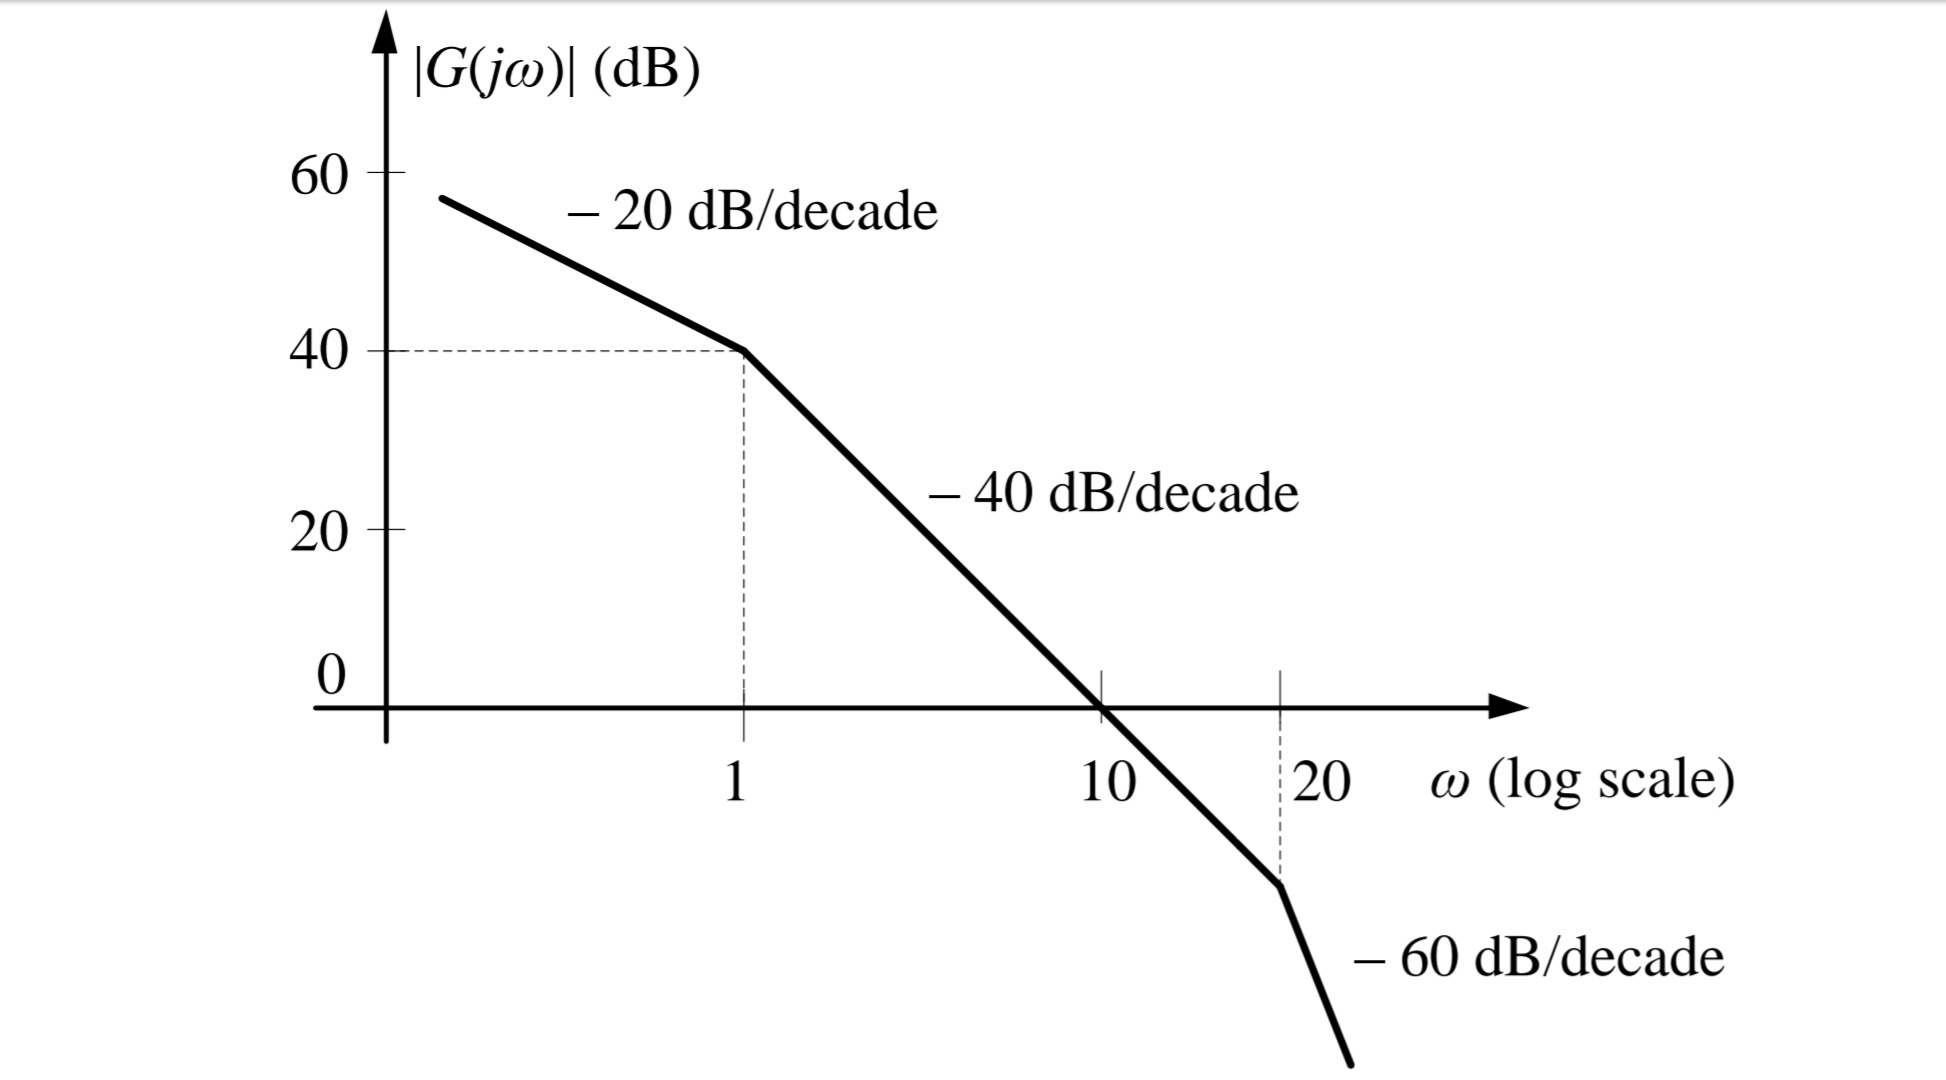
\includegraphics[width=\columnwidth]{./figs/ee18btech11009/pppp.eps}
	\caption{}
	\label{fig:ee18btech11009_bode}
\end{figure} 
%
Express $20\log\abs{G(\j\omega)}$ as a function of $\omega$ using Fig. \ref{fig:ee18btech11009_bode}.
\label{prob:ee18btech11009_bode}
\\
\solution The desired expression (in dB) is
{\footnotesize
\begin{align}
 \abs{G(j\omega)} = 
 \begin{cases}
	60-20(\log(\omega)-\log(0.1)) &   0.1 < \omega < 1 \\
	80-40(\log(\omega)-\log(0.1)) &   1 < \omega < 20 \\
	126.02-60(\log(\omega)-\log(0.1)) &   20 < \omega   
 \end{cases}
\end{align}
}
\item Express the slope of $20\log\abs{G(\j\omega)}$ as a function of $\omega$. 
\\
\solution The desired slope is
\begin{align}
 \nabla20\log\abs{G(j\omega)} = 
 \begin{cases}
	-20 &  \omega < 1 \\
	-40 & 1 < \omega < 20 \\
	-60 & 20 < \omega   
 \end{cases}
\end{align}

\item Express the change of slope of $20\log\abs{G(\j\omega)}$ as a function of $\omega$. 
\\
\solution 
\begin{align}
 \Delta(\nabla20\log\abs{G(j\omega)}) = 
 \begin{cases}
    -20 &  \omega = 0 \\
	-20 &  \omega = 1 \\
	-20 &  \omega = 20
 \end{cases}
\label{eq:ee18btech11009_slope_change}
\end{align}
\item Find the poles and zeros of $G(s)$.
\\
\solution From \eqref{eq:ee18btech11009_slope_change}, the poles are located at 0,1,20. There are no zeros.
\item Find $G(s)$
\\
\solution 
\begin{align}
	G(s) = \frac{k}{s(1+s)(20+s)}
\end{align}

\item Obtain the Bode plot of $G(s)$ through a python code and compare with the line plot of the expression that you obtained in Problem \ref{prob:ee18btech11009_bode}
\solution Fig. \ref{fig:ee10btech11009_line_plot} shows the Bode plot of the transfer function obtained.
 The \textbf{Line plot} is the approximation of the \textbf{caluculated bode plot}. 
\begin{figure}[htp]
	\centering
	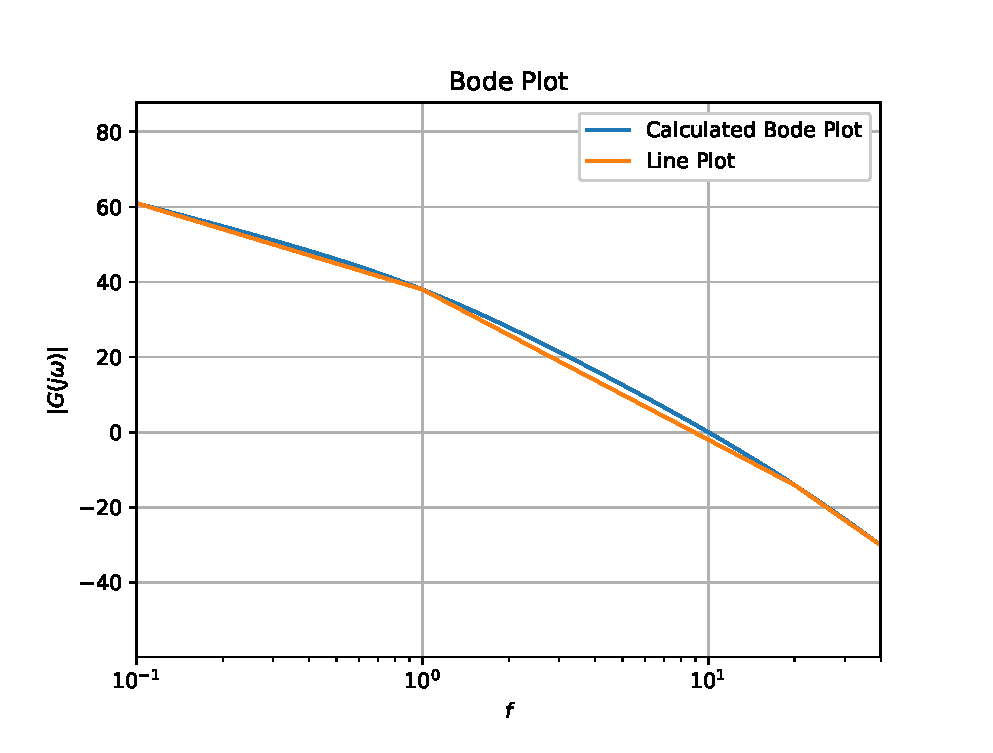
\includegraphics[width= \columnwidth]{./figs/ee18btech11009/ee18btech11009.eps}
	\caption{}
	\label{fig:ee10btech11009_line_plot}
\end{figure} 

\item  Verify if at very high frequency $(\omega \to \infty)$, the phase angle $ \angle G(j\omega)=-3\pi/2$.
\\
\solution
Phase $ \phi $ is the sum of all the phases corresponding to each pole and zero.
%------------------------------------------------
  \begin{align}
 \Rightarrow  G(j\omega) &=  \frac{k}{j\omega(1+j\omega)(20+j\omega)}
\\
\implies  \phi &=  -\tan^{-1}\brak{ {\frac{\omega}{0}}} - \tan^{-1}\brak{\omega} 
\nonumber\\
& \quad - \tan^{-1}\brak{ \frac{\omega}{20}}
\\
 & =  - 90\degree - \tan^{-1}\brak{\omega} - \tan^{-1}\brak{ \frac{\omega}{20}}
\\
\implies  \lim_{\omega \to \infty}   \phi &=    -3\pi/2 
 \end{align} 

 \end{enumerate}

\section{Second order System}
\subsection{Damping}
\begin{enumerate}[label=\thesubsection.\arabic*.,ref=\thesubsection.\theenumi]
\numberwithin{equation}{enumi}
\item List the different kinds of damping for a second order system defined by 
\begin{align}
\label{eq:ee18btech11012_second}
H(s)=\frac{\omega^2}{s^2+2\zeta\omega+\omega^2}
\end{align}
where $\omega$ is  the natural   frequency  and $ \zeta $  is the  damping factor.
%
\\
\solution The details are available in Table \ref{table:ee18btech11012}
\begin{table}[!ht]
\centering
\begin{enumerate}[label=\thesubsection.\arabic*.,ref=\thesubsection.\theenumi]
\numberwithin{equation}{enumi}
\item List the different kinds of damping for a second order system defined by 
\begin{align}
\label{eq:ee18btech11012_second}
H(s)=\frac{\omega^2}{s^2+2\zeta\omega+\omega^2}
\end{align}
where $\omega$ is  the natural   frequency  and $ \zeta $  is the  damping factor.
%
\\
\solution The details are available in Table \ref{table:ee18btech11012}
\begin{table}[!ht]
\centering
\begin{enumerate}[label=\thesubsection.\arabic*.,ref=\thesubsection.\theenumi]
\numberwithin{equation}{enumi}
\item List the different kinds of damping for a second order system defined by 
\begin{align}
\label{eq:ee18btech11012_second}
H(s)=\frac{\omega^2}{s^2+2\zeta\omega+\omega^2}
\end{align}
where $\omega$ is  the natural   frequency  and $ \zeta $  is the  damping factor.
%
\\
\solution The details are available in Table \ref{table:ee18btech11012}
\begin{table}[!ht]
\centering
\input{./tables/ee18btech11012.tex}
\caption{}
\label{table:ee18btech11012}
\end{table}

\item Classify the following second-order systems according to damping.
\label{prob:ee18btech11012_damp}
\begin{enumerate}
\item $H(s) = \frac{15}{{s^2+5s+15}}$ 
\item $H(s) = \frac{25}{{s^2+10s+25}}$
\item $H(s) =\frac{35}{{s^2+18s+35}}$ 
\end{enumerate}
\solution For 
\begin{align}
H(s) &= \frac{25}{{s^2+10s+25}},
\\
     \omega^2 &= 25,   2\zeta\omega =10\\
\implies  \omega &=1,  {\zeta} = 1
\end{align}
and the system is critically damped.  Similarly, the damping factors for other systems in Problem \ref{prob:ee18btech11012_damp} are calculated and listed in Table \ref{table:ee18btech11012_damp}
%
\begin{table}[!ht]
\centering
\input{./tables/ee18btech11012_damp.tex}
\caption{}
\label{table:ee18btech11012_damp}
\end{table}

\item Find the step response of each $H(s)$ in Table \ref{table:ee18btech11012_damp}.
\\
\solution 
\begin{enumerate}
\item For 
\begin{align}
 H(s)=\frac{15}{s^2+5s+15},
\end{align}
%
the step response is
\begin{equation}
y(t)=25te^{-5t}u(t)
\label{eq:ee18btech11012_over}
\end{equation}
\item For 
%
\begin{align}
H(s)=\frac{25}{s^2+10s+25},
\end{align}
%
the step response is
\begin{equation}
y(t)=\frac{30}{\sqrt{35}}e^{\frac{-5t}{2}}\sin\brak{\frac{\sqrt{35}}{2}t}u(t)
\label{eq:ee18btech11012_critical}
\end{equation}
\item  For 

\begin{align}
H(s)=\frac{35}{s^2+18s+35},
\end{align}
the step response is
\begin{equation}
    y(t)=\frac{35}{2\sqrt{46}}\sbrak{e^{(-9+\sqrt{46})t}-e^{(-9-\sqrt{46})t}}u(t)
\label{eq:ee18btech11012_under}
\end{equation}
\end{enumerate}
\item Illustrate the effect of damping by plotting the step responses in \eqref{eq:ee18btech11012_over}-\eqref{eq:ee18btech11012_under}
\\
\solution The following code
\begin{lstlisting}
codes/ee18btech11012.py
\end{lstlisting}
%
plots the desired graphs in
Fig.     \ref{fig:ee18btech11012}. 
%
%\begin{figure}[ht!]
%    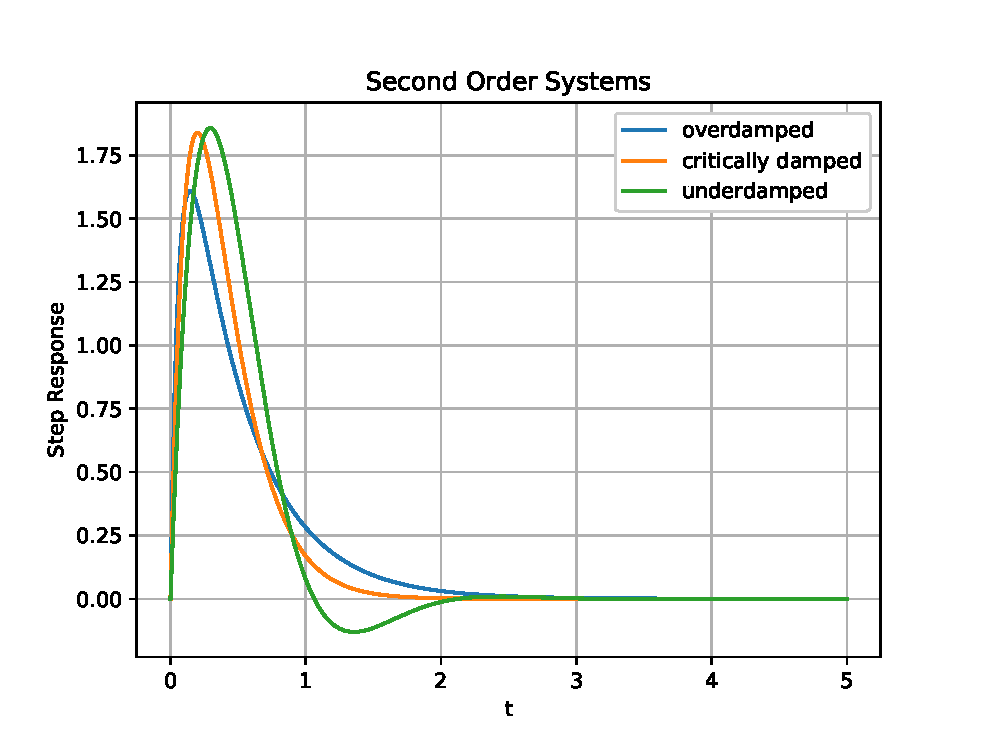
\includegraphics[width=\columnwidth]{./figs/ee18btech11012.eps}
%    \caption{}
%    \label{fig:ee18btech11012}
%\end{figure}

using a Python code to sketch the response.  
\end{enumerate}

\caption{}
\label{table:ee18btech11012}
\end{table}

\item Classify the following second-order systems according to damping.
\label{prob:ee18btech11012_damp}
\begin{enumerate}
\item $H(s) = \frac{15}{{s^2+5s+15}}$ 
\item $H(s) = \frac{25}{{s^2+10s+25}}$
\item $H(s) =\frac{35}{{s^2+18s+35}}$ 
\end{enumerate}
\solution For 
\begin{align}
H(s) &= \frac{25}{{s^2+10s+25}},
\\
     \omega^2 &= 25,   2\zeta\omega =10\\
\implies  \omega &=1,  {\zeta} = 1
\end{align}
and the system is critically damped.  Similarly, the damping factors for other systems in Problem \ref{prob:ee18btech11012_damp} are calculated and listed in Table \ref{table:ee18btech11012_damp}
%
\begin{table}[!ht]
\centering
%%%%%%%%%%%%%%%%%%%%%%%%%%%%%%%%%%%%%%%%%%%%%%%%%%%%%%%%%%%%%%%%%%%%%%
%%                                                                  %%
%%  This is the header of a LaTeX2e file exported from Gnumeric.    %%
%%                                                                  %%
%%  This file can be compiled as it stands or included in another   %%
%%  LaTeX document. The table is based on the longtable package so  %%
%%  the longtable options (headers, footers...) can be set in the   %%
%%  preamble section below (see PRAMBLE).                           %%
%%                                                                  %%
%%  To include the file in another, the following two lines must be %%
%%  in the including file:                                          %%
%%        \def\inputGnumericTable{}                                 %%
%%  at the beginning of the file and:                               %%
%%        \input{name-of-this-file.tex}                             %%
%%  where the table is to be placed. Note also that the including   %%
%%  file must use the following packages for the table to be        %%
%%  rendered correctly:                                             %%
%%    \usepackage[latin1]{inputenc}                                 %%
%%    \usepackage{color}                                            %%
%%    \usepackage{array}                                            %%
%%    \usepackage{longtable}                                        %%
%%    \usepackage{calc}                                             %%
%%    \usepackage{multirow}                                         %%
%%    \usepackage{hhline}                                           %%
%%    \usepackage{ifthen}                                           %%
%%  optionally (for landscape tables embedded in another document): %%
%%    \usepackage{lscape}                                           %%
%%                                                                  %%
%%%%%%%%%%%%%%%%%%%%%%%%%%%%%%%%%%%%%%%%%%%%%%%%%%%%%%%%%%%%%%%%%%%%%%



%%  This section checks if we are begin input into another file or  %%
%%  the file will be compiled alone. First use a macro taken from   %%
%%  the TeXbook ex 7.7 (suggestion of Han-Wen Nienhuys).            %%
\def\ifundefined#1{\expandafter\ifx\csname#1\endcsname\relax}


%%  Check for the \def token for inputed files. If it is not        %%
%%  defined, the file will be processed as a standalone and the     %%
%%  preamble will be used.                                          %%
\ifundefined{inputGnumericTable}

%%  We must be able to close or not the document at the end.        %%
	\def\gnumericTableEnd{\end{document}}


%%%%%%%%%%%%%%%%%%%%%%%%%%%%%%%%%%%%%%%%%%%%%%%%%%%%%%%%%%%%%%%%%%%%%%
%%                                                                  %%
%%  This is the PREAMBLE. Change these values to get the right      %%
%%  paper size and other niceties.                                  %%
%%                                                                  %%
%%%%%%%%%%%%%%%%%%%%%%%%%%%%%%%%%%%%%%%%%%%%%%%%%%%%%%%%%%%%%%%%%%%%%%

	\documentclass[12pt%
			  %,landscape%
                    ]{report}
       \usepackage[latin1]{inputenc}
       \usepackage{fullpage}
       \usepackage{color}
       \usepackage{array}
       \usepackage{longtable}
       \usepackage{calc}
       \usepackage{multirow}
       \usepackage{hhline}
       \usepackage{ifthen}

	\begin{document}


%%  End of the preamble for the standalone. The next section is for %%
%%  documents which are included into other LaTeX2e files.          %%
\else

%%  We are not a stand alone document. For a regular table, we will %%
%%  have no preamble and only define the closing to mean nothing.   %%
    \def\gnumericTableEnd{}

%%  If we want landscape mode in an embedded document, comment out  %%
%%  the line above and uncomment the two below. The table will      %%
%%  begin on a new page and run in landscape mode.                  %%
%       \def\gnumericTableEnd{\end{landscape}}
%       \begin{landscape}


%%  End of the else clause for this file being \input.              %%
\fi

%%%%%%%%%%%%%%%%%%%%%%%%%%%%%%%%%%%%%%%%%%%%%%%%%%%%%%%%%%%%%%%%%%%%%%
%%                                                                  %%
%%  The rest is the gnumeric table, except for the closing          %%
%%  statement. Changes below will alter the table's appearance.     %%
%%                                                                  %%
%%%%%%%%%%%%%%%%%%%%%%%%%%%%%%%%%%%%%%%%%%%%%%%%%%%%%%%%%%%%%%%%%%%%%%

\providecommand{\gnumericmathit}[1]{#1} 
%%  Uncomment the next line if you would like your numbers to be in %%
%%  italics if they are italizised in the gnumeric table.           %%
%\renewcommand{\gnumericmathit}[1]{\mathit{#1}}
\providecommand{\gnumericPB}[1]%
{\let\gnumericTemp=\\#1\let\\=\gnumericTemp\hspace{0pt}}
 \ifundefined{gnumericTableWidthDefined}
        \newlength{\gnumericTableWidth}
        \newlength{\gnumericTableWidthComplete}
        \newlength{\gnumericMultiRowLength}
        \global\def\gnumericTableWidthDefined{}
 \fi
%% The following setting protects this code from babel shorthands.  %%
 \ifthenelse{\isundefined{\languageshorthands}}{}{\languageshorthands{english}}
%%  The default table format retains the relative column widths of  %%
%%  gnumeric. They can easily be changed to c, r or l. In that case %%
%%  you may want to comment out the next line and uncomment the one %%
%%  thereafter                                                      %%
\providecommand\gnumbox{\makebox[0pt]}
%%\providecommand\gnumbox[1][]{\makebox}

%% to adjust positions in multirow situations                       %%
\setlength{\bigstrutjot}{\jot}
\setlength{\extrarowheight}{\doublerulesep}

%%  The \setlongtables command keeps column widths the same across  %%
%%  pages. Simply comment out next line for varying column widths.  %%
\setlongtables

\setlength\gnumericTableWidth{%
	36pt+%
	20pt+%
	35pt+%
	91pt+%
0pt}
\def\gumericNumCols{4}
\setlength\gnumericTableWidthComplete{\gnumericTableWidth+%
         \tabcolsep*\gumericNumCols*2+\arrayrulewidth*\gumericNumCols}
\ifthenelse{\lengthtest{\gnumericTableWidthComplete > \linewidth}}%
         {\def\gnumericScale{\ratio{\linewidth-%
                        \tabcolsep*\gumericNumCols*2-%
                        \arrayrulewidth*\gumericNumCols}%
{\gnumericTableWidth}}}%
{\def\gnumericScale{1}}

%%%%%%%%%%%%%%%%%%%%%%%%%%%%%%%%%%%%%%%%%%%%%%%%%%%%%%%%%%%%%%%%%%%%%%
%%                                                                  %%
%% The following are the widths of the various columns. We are      %%
%% defining them here because then they are easier to change.       %%
%% Depending on the cell formats we may use them more than once.    %%
%%                                                                  %%
%%%%%%%%%%%%%%%%%%%%%%%%%%%%%%%%%%%%%%%%%%%%%%%%%%%%%%%%%%%%%%%%%%%%%%

\ifthenelse{\isundefined{\gnumericColA}}{\newlength{\gnumericColA}}{}\settowidth{\gnumericColA}{\begin{tabular}{@{}p{36pt*\gnumericScale}@{}}x\end{tabular}}
\ifthenelse{\isundefined{\gnumericColB}}{\newlength{\gnumericColB}}{}\settowidth{\gnumericColB}{\begin{tabular}{@{}p{20pt*\gnumericScale}@{}}x\end{tabular}}
\ifthenelse{\isundefined{\gnumericColC}}{\newlength{\gnumericColC}}{}\settowidth{\gnumericColC}{\begin{tabular}{@{}p{35pt*\gnumericScale}@{}}x\end{tabular}}
\ifthenelse{\isundefined{\gnumericColD}}{\newlength{\gnumericColD}}{}\settowidth{\gnumericColD}{\begin{tabular}{@{}p{91pt*\gnumericScale}@{}}x\end{tabular}}

\begin{tabular}[c]{%
	b{\gnumericColA}%
	b{\gnumericColB}%
	b{\gnumericColC}%
	b{\gnumericColD}%
	}

%%%%%%%%%%%%%%%%%%%%%%%%%%%%%%%%%%%%%%%%%%%%%%%%%%%%%%%%%%%%%%%%%%%%%%
%%  The longtable options. (Caption, headers... see Goosens, p.124) %%
%	\caption{The Table Caption.}             \\	%
% \hline	% Across the top of the table.
%%  The rest of these options are table rows which are placed on    %%
%%  the first, last or every page. Use \multicolumn if you want.    %%

%%  Header for the first page.                                      %%
%	\multicolumn{4}{c}{The First Header} \\ \hline 
%	\multicolumn{1}{c}{colTag}	%Column 1
%	&\multicolumn{1}{c}{colTag}	%Column 2
%	&\multicolumn{1}{c}{colTag}	%Column 3
%	&\multicolumn{1}{c}{colTag}	\\ \hline %Last column
%	\endfirsthead

%%  The running header definition.                                  %%
%	\hline
%	\multicolumn{4}{l}{\ldots\small\slshape continued} \\ \hline
%	\multicolumn{1}{c}{colTag}	%Column 1
%	&\multicolumn{1}{c}{colTag}	%Column 2
%	&\multicolumn{1}{c}{colTag}	%Column 3
%	&\multicolumn{1}{c}{colTag}	\\ \hline %Last column
%	\endhead

%%  The running footer definition.                                  %%
%	\hline
%	\multicolumn{4}{r}{\small\slshape continued\ldots} \\
%	\endfoot

%%  The ending footer definition.                                   %%
%	\multicolumn{4}{c}{That's all folks} \\ \hline 
%	\endlastfoot
%%%%%%%%%%%%%%%%%%%%%%%%%%%%%%%%%%%%%%%%%%%%%%%%%%%%%%%%%%%%%%%%%%%%%%

\hhline{|-|-|-|-}
	 \multicolumn{1}{|p{\gnumericColA}|}%
	{\gnumericPB{\centering}\gnumbox{\textbf{H(s)}}}
	&\multicolumn{1}{p{\gnumericColB}|}%
	{\gnumericPB{\centering}\gnumbox{\textbf{$\omega$}}}
	&\multicolumn{1}{p{\gnumericColC}|}%
	{\gnumericPB{\centering}\gnumbox{\textbf{$\zeta$}}}
	&\multicolumn{1}{p{\gnumericColD}|}%
	{\gnumericPB{\raggedright}\gnumbox[l]{\textbf{Damping Type}}}
\\
\hhline{|----|}
	 \multicolumn{1}{|p{\gnumericColA}|}%
	{$\frac{35}{{s^2+18s+35}}$ }
	&\multicolumn{1}{p{\gnumericColB}|}%
	{$\sqrt{35}$}
	&\multicolumn{1}{p{\gnumericColC}|}%
	{\gnumericPB{\centering}\gnumbox{$\sqrt{\frac{81}{35}}> 1$}}
	&\multicolumn{1}{p{\gnumericColD}|}%
	{\gnumericPB{\raggedright}\gnumbox[l]{Overdamped}}
\\
\hhline{|----|}
	 \multicolumn{1}{|p{\gnumericColA}|}%
	{$\frac{25}{{s^2+10s+25}}$}
	&\multicolumn{1}{p{\gnumericColB}|}%
	{$5$}
	&\multicolumn{1}{p{\gnumericColC}|}%
	{\gnumericPB{\centering}\gnumbox{$1$}}
	&\multicolumn{1}{p{\gnumericColD}|}%
	{\gnumericPB{\raggedright}\gnumbox[l]{Critically Damped}}
\\
\hhline{|----|}
	 \multicolumn{1}{|p{\gnumericColA}|}%
	{$\frac{15}{{s^2+5s+15}}$}
	&\multicolumn{1}{p{\gnumericColB}|}%
	{$\sqrt{15}$}
	&\multicolumn{1}{p{\gnumericColC}|}%
	{\gnumericPB{\centering}\gnumbox{$\sqrt{\frac{5}{12}}< 1$}}
	&\multicolumn{1}{p{\gnumericColD}|}%
	{\gnumericPB{\raggedright}\gnumbox[l]{Underdamped}}
\\
\hhline{|-|-|-|-|}
\end{tabular}

\ifthenelse{\isundefined{\languageshorthands}}{}{\languageshorthands{\languagename}}
\gnumericTableEnd

\caption{}
\label{table:ee18btech11012_damp}
\end{table}

\item Find the step response of each $H(s)$ in Table \ref{table:ee18btech11012_damp}.
\\
\solution 
\begin{enumerate}
\item For 
\begin{align}
 H(s)=\frac{15}{s^2+5s+15},
\end{align}
%
the step response is
\begin{equation}
y(t)=25te^{-5t}u(t)
\label{eq:ee18btech11012_over}
\end{equation}
\item For 
%
\begin{align}
H(s)=\frac{25}{s^2+10s+25},
\end{align}
%
the step response is
\begin{equation}
y(t)=\frac{30}{\sqrt{35}}e^{\frac{-5t}{2}}\sin\brak{\frac{\sqrt{35}}{2}t}u(t)
\label{eq:ee18btech11012_critical}
\end{equation}
\item  For 

\begin{align}
H(s)=\frac{35}{s^2+18s+35},
\end{align}
the step response is
\begin{equation}
    y(t)=\frac{35}{2\sqrt{46}}\sbrak{e^{(-9+\sqrt{46})t}-e^{(-9-\sqrt{46})t}}u(t)
\label{eq:ee18btech11012_under}
\end{equation}
\end{enumerate}
\item Illustrate the effect of damping by plotting the step responses in \eqref{eq:ee18btech11012_over}-\eqref{eq:ee18btech11012_under}
\\
\solution The following code
\begin{lstlisting}
codes/ee18btech11012.py
\end{lstlisting}
%
plots the desired graphs in
Fig.     \ref{fig:ee18btech11012}. 
%
%\begin{figure}[ht!]
%    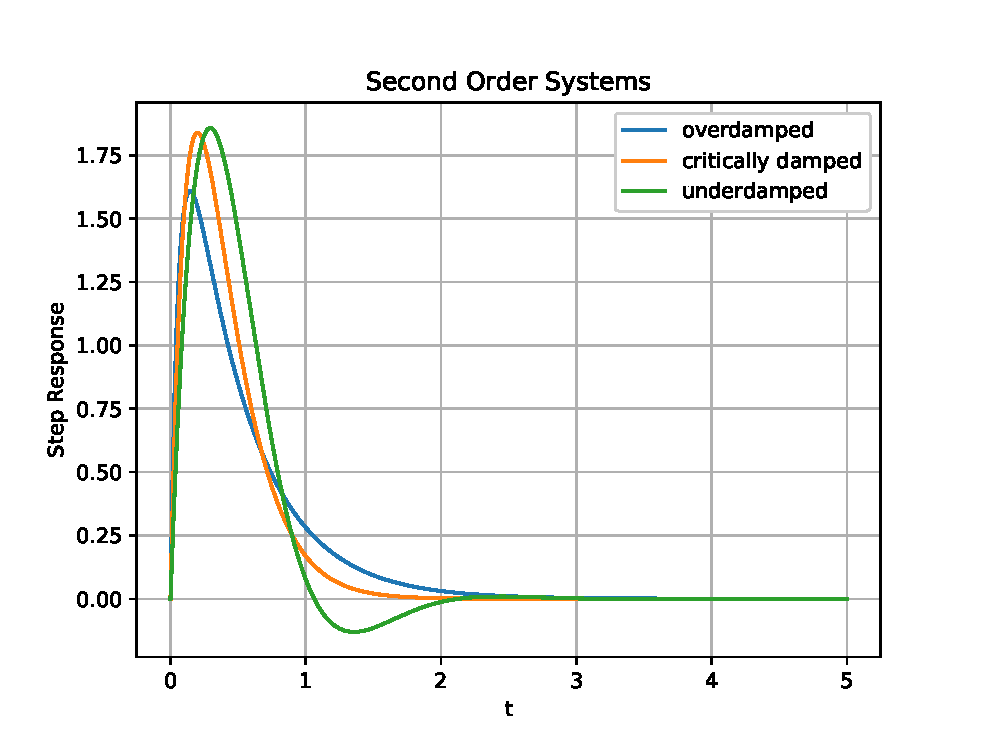
\includegraphics[width=\columnwidth]{./figs/ee18btech11012.eps}
%    \caption{}
%    \label{fig:ee18btech11012}
%\end{figure}

using a Python code to sketch the response.  
\end{enumerate}

\caption{}
\label{table:ee18btech11012}
\end{table}

\item Classify the following second-order systems according to damping.
\label{prob:ee18btech11012_damp}
\begin{enumerate}
\item $H(s) = \frac{15}{{s^2+5s+15}}$ 
\item $H(s) = \frac{25}{{s^2+10s+25}}$
\item $H(s) =\frac{35}{{s^2+18s+35}}$ 
\end{enumerate}
\solution For 
\begin{align}
H(s) &= \frac{25}{{s^2+10s+25}},
\\
     \omega^2 &= 25,   2\zeta\omega =10\\
\implies  \omega &=1,  {\zeta} = 1
\end{align}
and the system is critically damped.  Similarly, the damping factors for other systems in Problem \ref{prob:ee18btech11012_damp} are calculated and listed in Table \ref{table:ee18btech11012_damp}
%
\begin{table}[!ht]
\centering
%%%%%%%%%%%%%%%%%%%%%%%%%%%%%%%%%%%%%%%%%%%%%%%%%%%%%%%%%%%%%%%%%%%%%%
%%                                                                  %%
%%  This is the header of a LaTeX2e file exported from Gnumeric.    %%
%%                                                                  %%
%%  This file can be compiled as it stands or included in another   %%
%%  LaTeX document. The table is based on the longtable package so  %%
%%  the longtable options (headers, footers...) can be set in the   %%
%%  preamble section below (see PRAMBLE).                           %%
%%                                                                  %%
%%  To include the file in another, the following two lines must be %%
%%  in the including file:                                          %%
%%        \def\inputGnumericTable{}                                 %%
%%  at the beginning of the file and:                               %%
%%        \input{name-of-this-file.tex}                             %%
%%  where the table is to be placed. Note also that the including   %%
%%  file must use the following packages for the table to be        %%
%%  rendered correctly:                                             %%
%%    \usepackage[latin1]{inputenc}                                 %%
%%    \usepackage{color}                                            %%
%%    \usepackage{array}                                            %%
%%    \usepackage{longtable}                                        %%
%%    \usepackage{calc}                                             %%
%%    \usepackage{multirow}                                         %%
%%    \usepackage{hhline}                                           %%
%%    \usepackage{ifthen}                                           %%
%%  optionally (for landscape tables embedded in another document): %%
%%    \usepackage{lscape}                                           %%
%%                                                                  %%
%%%%%%%%%%%%%%%%%%%%%%%%%%%%%%%%%%%%%%%%%%%%%%%%%%%%%%%%%%%%%%%%%%%%%%



%%  This section checks if we are begin input into another file or  %%
%%  the file will be compiled alone. First use a macro taken from   %%
%%  the TeXbook ex 7.7 (suggestion of Han-Wen Nienhuys).            %%
\def\ifundefined#1{\expandafter\ifx\csname#1\endcsname\relax}


%%  Check for the \def token for inputed files. If it is not        %%
%%  defined, the file will be processed as a standalone and the     %%
%%  preamble will be used.                                          %%
\ifundefined{inputGnumericTable}

%%  We must be able to close or not the document at the end.        %%
	\def\gnumericTableEnd{\end{document}}


%%%%%%%%%%%%%%%%%%%%%%%%%%%%%%%%%%%%%%%%%%%%%%%%%%%%%%%%%%%%%%%%%%%%%%
%%                                                                  %%
%%  This is the PREAMBLE. Change these values to get the right      %%
%%  paper size and other niceties.                                  %%
%%                                                                  %%
%%%%%%%%%%%%%%%%%%%%%%%%%%%%%%%%%%%%%%%%%%%%%%%%%%%%%%%%%%%%%%%%%%%%%%

	\documentclass[12pt%
			  %,landscape%
                    ]{report}
       \usepackage[latin1]{inputenc}
       \usepackage{fullpage}
       \usepackage{color}
       \usepackage{array}
       \usepackage{longtable}
       \usepackage{calc}
       \usepackage{multirow}
       \usepackage{hhline}
       \usepackage{ifthen}

	\begin{document}


%%  End of the preamble for the standalone. The next section is for %%
%%  documents which are included into other LaTeX2e files.          %%
\else

%%  We are not a stand alone document. For a regular table, we will %%
%%  have no preamble and only define the closing to mean nothing.   %%
    \def\gnumericTableEnd{}

%%  If we want landscape mode in an embedded document, comment out  %%
%%  the line above and uncomment the two below. The table will      %%
%%  begin on a new page and run in landscape mode.                  %%
%       \def\gnumericTableEnd{\end{landscape}}
%       \begin{landscape}


%%  End of the else clause for this file being \input.              %%
\fi

%%%%%%%%%%%%%%%%%%%%%%%%%%%%%%%%%%%%%%%%%%%%%%%%%%%%%%%%%%%%%%%%%%%%%%
%%                                                                  %%
%%  The rest is the gnumeric table, except for the closing          %%
%%  statement. Changes below will alter the table's appearance.     %%
%%                                                                  %%
%%%%%%%%%%%%%%%%%%%%%%%%%%%%%%%%%%%%%%%%%%%%%%%%%%%%%%%%%%%%%%%%%%%%%%

\providecommand{\gnumericmathit}[1]{#1} 
%%  Uncomment the next line if you would like your numbers to be in %%
%%  italics if they are italizised in the gnumeric table.           %%
%\renewcommand{\gnumericmathit}[1]{\mathit{#1}}
\providecommand{\gnumericPB}[1]%
{\let\gnumericTemp=\\#1\let\\=\gnumericTemp\hspace{0pt}}
 \ifundefined{gnumericTableWidthDefined}
        \newlength{\gnumericTableWidth}
        \newlength{\gnumericTableWidthComplete}
        \newlength{\gnumericMultiRowLength}
        \global\def\gnumericTableWidthDefined{}
 \fi
%% The following setting protects this code from babel shorthands.  %%
 \ifthenelse{\isundefined{\languageshorthands}}{}{\languageshorthands{english}}
%%  The default table format retains the relative column widths of  %%
%%  gnumeric. They can easily be changed to c, r or l. In that case %%
%%  you may want to comment out the next line and uncomment the one %%
%%  thereafter                                                      %%
\providecommand\gnumbox{\makebox[0pt]}
%%\providecommand\gnumbox[1][]{\makebox}

%% to adjust positions in multirow situations                       %%
\setlength{\bigstrutjot}{\jot}
\setlength{\extrarowheight}{\doublerulesep}

%%  The \setlongtables command keeps column widths the same across  %%
%%  pages. Simply comment out next line for varying column widths.  %%
\setlongtables

\setlength\gnumericTableWidth{%
	36pt+%
	20pt+%
	35pt+%
	91pt+%
0pt}
\def\gumericNumCols{4}
\setlength\gnumericTableWidthComplete{\gnumericTableWidth+%
         \tabcolsep*\gumericNumCols*2+\arrayrulewidth*\gumericNumCols}
\ifthenelse{\lengthtest{\gnumericTableWidthComplete > \linewidth}}%
         {\def\gnumericScale{\ratio{\linewidth-%
                        \tabcolsep*\gumericNumCols*2-%
                        \arrayrulewidth*\gumericNumCols}%
{\gnumericTableWidth}}}%
{\def\gnumericScale{1}}

%%%%%%%%%%%%%%%%%%%%%%%%%%%%%%%%%%%%%%%%%%%%%%%%%%%%%%%%%%%%%%%%%%%%%%
%%                                                                  %%
%% The following are the widths of the various columns. We are      %%
%% defining them here because then they are easier to change.       %%
%% Depending on the cell formats we may use them more than once.    %%
%%                                                                  %%
%%%%%%%%%%%%%%%%%%%%%%%%%%%%%%%%%%%%%%%%%%%%%%%%%%%%%%%%%%%%%%%%%%%%%%

\ifthenelse{\isundefined{\gnumericColA}}{\newlength{\gnumericColA}}{}\settowidth{\gnumericColA}{\begin{tabular}{@{}p{36pt*\gnumericScale}@{}}x\end{tabular}}
\ifthenelse{\isundefined{\gnumericColB}}{\newlength{\gnumericColB}}{}\settowidth{\gnumericColB}{\begin{tabular}{@{}p{20pt*\gnumericScale}@{}}x\end{tabular}}
\ifthenelse{\isundefined{\gnumericColC}}{\newlength{\gnumericColC}}{}\settowidth{\gnumericColC}{\begin{tabular}{@{}p{35pt*\gnumericScale}@{}}x\end{tabular}}
\ifthenelse{\isundefined{\gnumericColD}}{\newlength{\gnumericColD}}{}\settowidth{\gnumericColD}{\begin{tabular}{@{}p{91pt*\gnumericScale}@{}}x\end{tabular}}

\begin{tabular}[c]{%
	b{\gnumericColA}%
	b{\gnumericColB}%
	b{\gnumericColC}%
	b{\gnumericColD}%
	}

%%%%%%%%%%%%%%%%%%%%%%%%%%%%%%%%%%%%%%%%%%%%%%%%%%%%%%%%%%%%%%%%%%%%%%
%%  The longtable options. (Caption, headers... see Goosens, p.124) %%
%	\caption{The Table Caption.}             \\	%
% \hline	% Across the top of the table.
%%  The rest of these options are table rows which are placed on    %%
%%  the first, last or every page. Use \multicolumn if you want.    %%

%%  Header for the first page.                                      %%
%	\multicolumn{4}{c}{The First Header} \\ \hline 
%	\multicolumn{1}{c}{colTag}	%Column 1
%	&\multicolumn{1}{c}{colTag}	%Column 2
%	&\multicolumn{1}{c}{colTag}	%Column 3
%	&\multicolumn{1}{c}{colTag}	\\ \hline %Last column
%	\endfirsthead

%%  The running header definition.                                  %%
%	\hline
%	\multicolumn{4}{l}{\ldots\small\slshape continued} \\ \hline
%	\multicolumn{1}{c}{colTag}	%Column 1
%	&\multicolumn{1}{c}{colTag}	%Column 2
%	&\multicolumn{1}{c}{colTag}	%Column 3
%	&\multicolumn{1}{c}{colTag}	\\ \hline %Last column
%	\endhead

%%  The running footer definition.                                  %%
%	\hline
%	\multicolumn{4}{r}{\small\slshape continued\ldots} \\
%	\endfoot

%%  The ending footer definition.                                   %%
%	\multicolumn{4}{c}{That's all folks} \\ \hline 
%	\endlastfoot
%%%%%%%%%%%%%%%%%%%%%%%%%%%%%%%%%%%%%%%%%%%%%%%%%%%%%%%%%%%%%%%%%%%%%%

\hhline{|-|-|-|-}
	 \multicolumn{1}{|p{\gnumericColA}|}%
	{\gnumericPB{\centering}\gnumbox{\textbf{H(s)}}}
	&\multicolumn{1}{p{\gnumericColB}|}%
	{\gnumericPB{\centering}\gnumbox{\textbf{$\omega$}}}
	&\multicolumn{1}{p{\gnumericColC}|}%
	{\gnumericPB{\centering}\gnumbox{\textbf{$\zeta$}}}
	&\multicolumn{1}{p{\gnumericColD}|}%
	{\gnumericPB{\raggedright}\gnumbox[l]{\textbf{Damping Type}}}
\\
\hhline{|----|}
	 \multicolumn{1}{|p{\gnumericColA}|}%
	{$\frac{35}{{s^2+18s+35}}$ }
	&\multicolumn{1}{p{\gnumericColB}|}%
	{$\sqrt{35}$}
	&\multicolumn{1}{p{\gnumericColC}|}%
	{\gnumericPB{\centering}\gnumbox{$\sqrt{\frac{81}{35}}> 1$}}
	&\multicolumn{1}{p{\gnumericColD}|}%
	{\gnumericPB{\raggedright}\gnumbox[l]{Overdamped}}
\\
\hhline{|----|}
	 \multicolumn{1}{|p{\gnumericColA}|}%
	{$\frac{25}{{s^2+10s+25}}$}
	&\multicolumn{1}{p{\gnumericColB}|}%
	{$5$}
	&\multicolumn{1}{p{\gnumericColC}|}%
	{\gnumericPB{\centering}\gnumbox{$1$}}
	&\multicolumn{1}{p{\gnumericColD}|}%
	{\gnumericPB{\raggedright}\gnumbox[l]{Critically Damped}}
\\
\hhline{|----|}
	 \multicolumn{1}{|p{\gnumericColA}|}%
	{$\frac{15}{{s^2+5s+15}}$}
	&\multicolumn{1}{p{\gnumericColB}|}%
	{$\sqrt{15}$}
	&\multicolumn{1}{p{\gnumericColC}|}%
	{\gnumericPB{\centering}\gnumbox{$\sqrt{\frac{5}{12}}< 1$}}
	&\multicolumn{1}{p{\gnumericColD}|}%
	{\gnumericPB{\raggedright}\gnumbox[l]{Underdamped}}
\\
\hhline{|-|-|-|-|}
\end{tabular}

\ifthenelse{\isundefined{\languageshorthands}}{}{\languageshorthands{\languagename}}
\gnumericTableEnd

\caption{}
\label{table:ee18btech11012_damp}
\end{table}

\item Find the step response of each $H(s)$ in Table \ref{table:ee18btech11012_damp}.
\\
\solution 
\begin{enumerate}
\item For 
\begin{align}
 H(s)=\frac{15}{s^2+5s+15},
\end{align}
%
the step response is
\begin{equation}
y(t)=25te^{-5t}u(t)
\label{eq:ee18btech11012_over}
\end{equation}
\item For 
%
\begin{align}
H(s)=\frac{25}{s^2+10s+25},
\end{align}
%
the step response is
\begin{equation}
y(t)=\frac{30}{\sqrt{35}}e^{\frac{-5t}{2}}\sin\brak{\frac{\sqrt{35}}{2}t}u(t)
\label{eq:ee18btech11012_critical}
\end{equation}
\item  For 

\begin{align}
H(s)=\frac{35}{s^2+18s+35},
\end{align}
the step response is
\begin{equation}
    y(t)=\frac{35}{2\sqrt{46}}\sbrak{e^{(-9+\sqrt{46})t}-e^{(-9-\sqrt{46})t}}u(t)
\label{eq:ee18btech11012_under}
\end{equation}
\end{enumerate}
\item Illustrate the effect of damping by plotting the step responses in \eqref{eq:ee18btech11012_over}-\eqref{eq:ee18btech11012_under}
\\
\solution The following code
\begin{lstlisting}
codes/ee18btech11012.py
\end{lstlisting}
%
plots the desired graphs in
Fig.     \ref{fig:ee18btech11012}. 
%
%\begin{figure}[ht!]
%    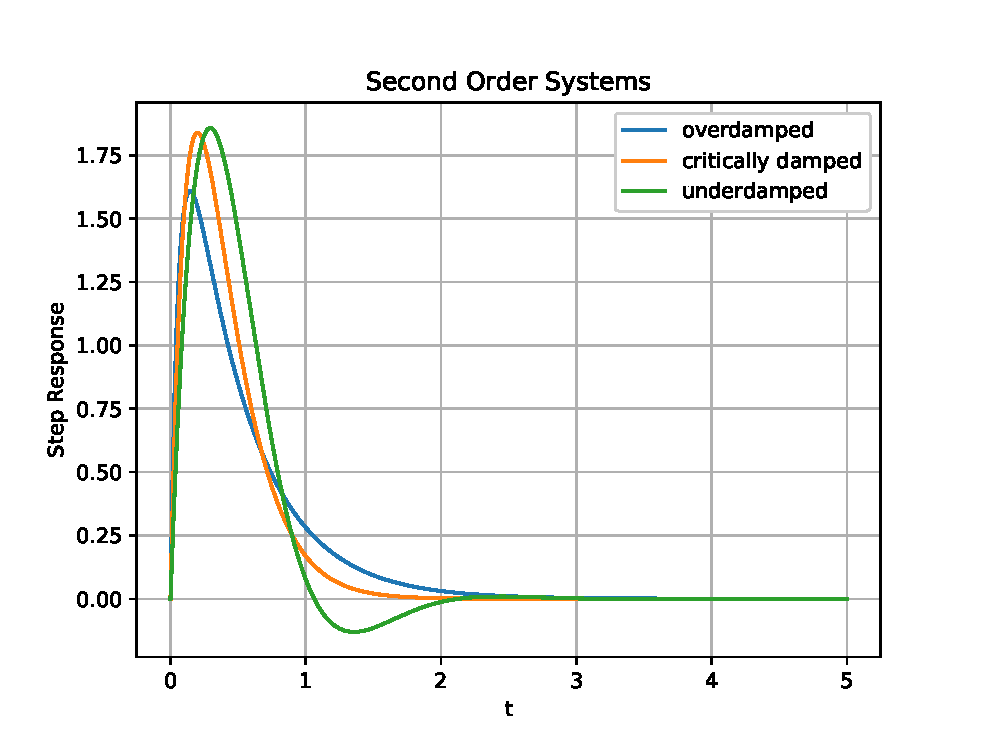
\includegraphics[width=\columnwidth]{./figs/ee18btech11012.eps}
%    \caption{}
%    \label{fig:ee18btech11012}
%\end{figure}

using a Python code to sketch the response.  
\end{enumerate}

\subsection{Example}
%\begin{enumerate}[label=\thesection.\arabic*.,ref=\thesection.\theenumi]
%\numberwithin{equation}{enumi}
%\item 
Sketch the direct polar plot for a unity feedback system with open loop transfer function
\begin{align}
\label{eq:ee18btech11002_gain}
G(s) = \frac{1}{s(1+s)^2}
\end{align}
\\
\solution  
The polar plot is obtained by plotting $\brak{r,\phi}$
\begin{align}
r&=|H(\j\omega)||G(\j\omega)|
\\
\phi&=\angle H(\j\omega)G(\j\omega), 0 < \omega < \infty
\end{align}
The following code plots the polar plot in Fig. \ref{fig:ee18btech11002polar_plot}

\begin{lstlisting}
codes/ee18btech11002/polarplot.py
\end{lstlisting}
\begin{figure}[!ht]
\centering
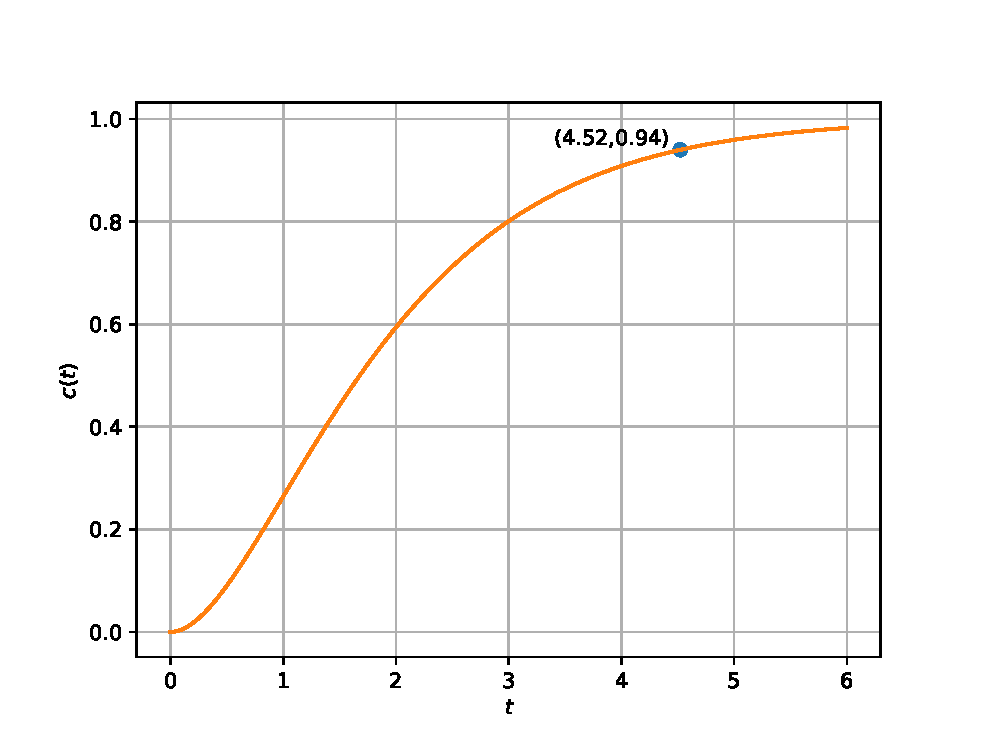
\includegraphics[width=\columnwidth]{./figs/ee18btech11002/ee18btech11002.eps}
\caption{Polar Plot}
\label{fig:ee18btech11002polar_plot}
\end{figure}
%\item 
Sketch the inverse polar plot for \eqref{eq:ee18btech11002_gain}
\\
\solution The above code plots the polar plot in Fig. \ref{fig:ee18btech11002inverse_polar_plot} by plotting  $\brak{\frac{1}{r}r,-\phi}$

%
\begin{figure}
\centering
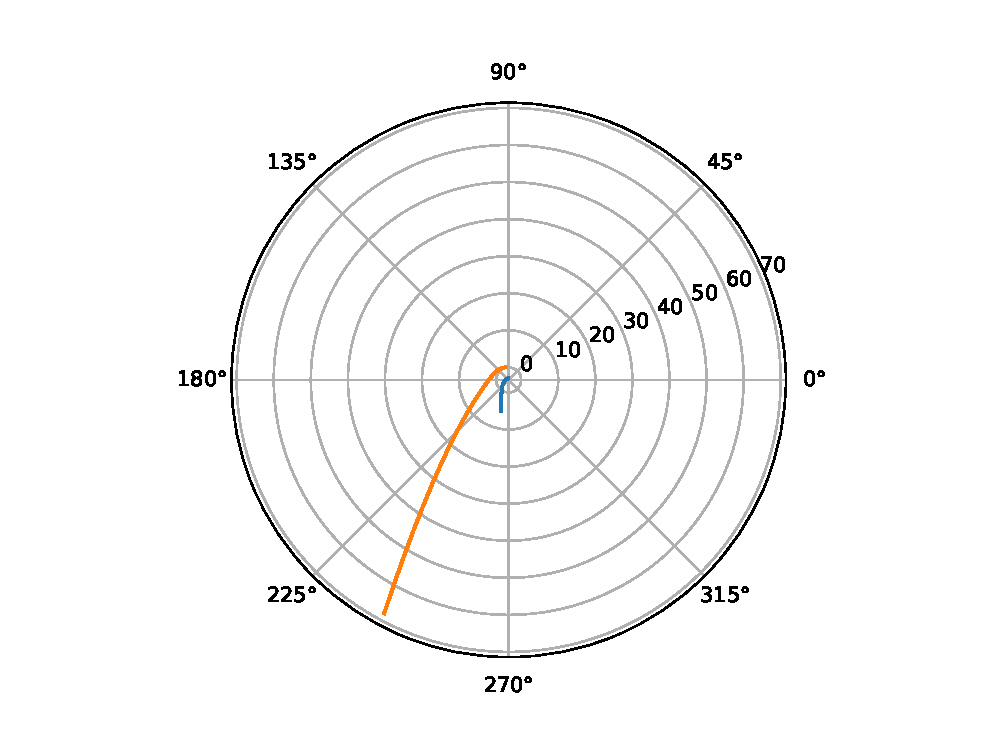
\includegraphics[width=\columnwidth]{./figs/ee18btech11002/ee18btech11002_1.eps}
\caption{Inverse Polar Plot}
\label{fig:ee18btech11002inverse_polar_plot}
\end{figure}


%\end{enumerate}

\section{Routh Hurwitz Criterion}
\subsection{Routh Array}
%\begin{enumerate}[label=\arabic*.,ref=\theenumi]
\begin{enumerate}[label=\thesection.\arabic*.,ref=\thesection.\theenumi]
\numberwithin{equation}{enumi}
%2.1.1
\item Consider the Magnitude Bode Plot and Phase Bode Plot \ref{fig:ee18btech11014_Bode} of Open-Loop Transfer Function of an Amplifier. Estimate the Open-Loop Transfer Function. (Assume $'A'$ as $'G'$ and $'\beta'$ as $'H'$)
\begin{figure}[ht!]
	\begin{center}
		\includegraphics[width=\columnwidth]{./figs/ee18btech11014/ee18btech11014_figa.eps}
	\end{center}
	\caption{Magnitude and Phase Bode Plot}
	\label{fig:ee18btech11014_Bode}
\end{figure}
\\
\solution Let $G(f)$ be the Open-Loop Transfer Function,
\begin{align}
G(f) = 
\begin{cases} 
      100 & 0 < f < 10^{5} \\
      200-20\log(f) & 10^{5} < f < 10^{6} \\
      320-40\log(f) & 10^{6} < f < 10^{7} \\
      460-60\log(f) & 10^{7} < f  \\
\end{cases}
\end{align}

\begin{align}
\nabla G(f) &= \dfrac{d(G(f))}{d(\log(f))} =
\begin{cases} 
        0 & 0 < f < 10^{5} \\
      -20 & 10^{5} < f < 10^{6} \\
      -40 & 10^{6} < f < 10^{7} \\
      -60 & 10^{7} < f  \\ 
\end{cases}
\end{align}

As we know that, \textbf{When a pole is encountered the slope always decreases by 20 dB/decade} and \textbf{When a zero is encountered the slope always increases by 20 dB/decade}. So, by observing Fig. \ref{fig:ee18btech11014_Bode} it can be concluded that we are having Poles at $f=10^{5} Hz, 10^{6} Hz, 10^{7} Hz$ and No Zeros.\\

So, the Open-Loop Transfer Function $G(f)$ is
\begin{align}
\label{eq:ee18btech11014_G}
	G(f) = \dfrac{10^{5}}{\left(1+j\frac{f}{10^{5}}\right)\left(1+j\frac{f}{10^{6}}\right)\left(1+j\frac{f}{10^{7}}\right)}
\end{align}\\
%-------------------------------------------------------------------------------------------------%
%2.1.2
\item Calculate the Phase of Open-Loop Transfer Function.\\
\solution
%
\begin{multline}
\label{eq:ee18btech11014_G_ang}
\phi\brak{f} =
\\
-\sbrak{\tan ^{-1}\brak{\frac{f}{10^{5}}}+\tan ^{-1}\brak{\frac{f}{10^{6}}}+\tan ^{-1}\brak{\frac{f}{10^{7}}}}
\end{multline}
%-------------------------------------------------------------------------------------------------%
%2.1.3
\item Find the PM from  Fig. 	\ref{fig:ee18btech11014_Bode}, given that he feedback gain $H(f)$ is constant and given by 
\begin{align}
20 \log \brak{\frac{1}{H(f) }} &= 85 dB
\\
\text{or, } H(f) &= 5.623 \times 10^{-5}.
\end{align}
\\
\solution From the figure, 
\begin{align}
\label{eq:ee18btech11014_G_f1}
20 \log \abs{G(f_1)} &= 85 dB
\\
\implies 20 \log \abs{G(f_1)} & = 20 \log \brak{\frac{1}{H(f_1) }}
\\
\text{or, } \abs{G(f_1)H(f_1)} &= 1
\end{align}
and 
\begin{align}
\label{eq:ee18btech11014_f1}
f_1 = 0.493 MHz, 
\end{align}
from \eqref{eq:ee18btech11014_G_f1} and \eqref{eq:ee18btech11014_G}.
Also,
%
\begin{align}
\because \phase{H(f)} &= 0, \forall f
\\
\phase{G(f_1)H(f_1)} &= \phase{G(f_1)} = -108 \degree
\\
\implies PM &= 180 \degree - 108 \degree = 72 \degree
\end{align}
using \eqref{eq:ee18btech11014_f1} in \eqref{eq:ee18btech11014_G_ang}.

%-------------------------------------------------------------------------------------------------%
\item Find the GM.
\\
\solution The crossover frequency $f_{\pi}$ is defined as 
\begin{align}
\phase{G\brak{f_{\pi}}H\brak{f_{\pi}}} &= 180 \degree
\\
\implies \phase{G\brak{f_{\pi}}} &= 180 \degree
\\
\implies f_{\pi} &= 3.34 MHz
\end{align}
by solving \eqref{eq:ee18btech11014_G_ang}.
From Fig. \ref{fig:ee18btech11014_Bode}, 
\begin{align}
\label{eq:ee18btech11014_G_f1}
20 \log \abs{G(f_\pi)} &= 60 dB
\\
\implies 20 \log \abs{G(f_\pi)} &-  20 \log \brak{\frac{1}{H(f_\pi) }}   
\nonumber \\
&= \brak{60 -85} dB
\\
\implies GM &= \abs{20 \log \abs{G(f_\pi)H(f_\pi) }} 
\nonumber \\
&= 25 dB
\end{align}
%

%------------------------------------------%
%2.1.8
\item Break the Transfer Function $G(f)$ into Simple Blocks and Create a Block Diagram for $G(f)$.\\
\solution\\
\begin{figure}[ht!]
	\begin{center}
		\resizebox{\columnwidth}{!}{\tikzstyle{block} = [draw, rectangle, 
    minimum height=1.5em, minimum width=3em]
\tikzstyle{sum} = [draw, circle, node distance=1cm]
\tikzstyle{input} = [coordinate]
\tikzstyle{output} = [coordinate]
\tikzstyle{pinstyle} = [pin edge={to-,thin,black}]

% The block diagram code is probably more verbose than necessary
\begin{tikzpicture}[auto, node distance=2.5cm,>=latex']
    % We start by placing the blocks
    \node [input, name=input] {};
    \node [block, right of=input] (g) {$10^{5}$};
    \node [block, right of=g] (p1) {$\frac{1}{1+\frac{s}{2\pi \times 10^{7}}}$};
    \node [block, right of=p1] (p2) {$\frac{1}{1+\frac{s}{2\pi \times 10^{6}}}$};
    \node [block, right of=p2] (p3) {$\frac{1}{1+\frac{s}{2\pi \times 10^{5}}}$};
    \node [output, right of=p3] (output) {};

    % Once the nodes are placed, connecting them is easy. 
    \draw [draw,->] (input) -- node {$v_{s}$} (g);
    \draw [->] (g) -- node {$v_{a}$} (p1);
    \draw [->] (p1) -- node {$v_{b}$} (p2);
    \draw [->] (p2) -- node {$v_{b}$} (p3);
    \draw [->] (p3) -- node {$v_{o}$} (output);
    
\end{tikzpicture}
}
	\end{center}
	\caption{}
	\label{fig:ee18btech11014_RC Circuit}
\end{figure}

%-------------------------------------------------------------------------------------------------%
%2.1.9
\item Find the Gain of RC-Circuit in Fig. \ref{fig:ee18btech11014_RC Circuit} and identify the pole location.
\begin{figure}[ht!]
	\begin{center}
		\resizebox{\columnwidth/2}{!}{\begin{circuitikz}[american]
\tikzset{quad/.style={draw, minimum height=2.4cm, minimum width=4cm}}
\node[quad] (A) at (0,0) {$H$};
\draw ($(A.north west)!.175!(A.west)$) to[short,-o] ++(-2,0) -- (-5,1)
      ($(A.south west)!.175!(A.west)$) to[short,-o] ++(-2,0) -- (-5,-1)
      ($(A.north east)!.175!(A.east)$) to[short,-o] ++(1,0)
      ($(A.south east)!.175!(A.east)$) to[short,-o] ++(1,0);

\draw (-5,-1) to[short, i=$I_{f}$] (-5,1);
\draw (-5,-1) to[closing switch, o-o] (-5,-2) node[ground](GND){};

\draw (3,-1) -- (5,-1) to[isource, l= $I_{o}$] (5,1) -- (3,1);

\end{circuitikz}
}
	\end{center}
	\caption{}
	\label{fig:ee18btech11014_RC Circuit}
\end{figure}

\solution
\begin{align}
v_o &= v_i \frac{\frac{1}{sc}}{R + \frac{1}{sC}}
\\
\implies \frac{v_o}{v_i}&= \frac{1}{1+sCR}
%I = \frac{v_{input}}{R + \frac{1}{Cs}}\\
%v_{output} = I \times \frac{1}{Cs}\\
%v_{output} = \frac{v_{input} \times \frac{1}{Cs}}{R + \frac{1}{Cs}}\\
%\frac{v_{output}}{v_{input}} = \frac{1}{RCs + 1}\\
%s = j2\pi f\\
%Gain = \frac{v_{output}}{v_{input}} = \frac{1}{j2\pi RCf + 1}
\end{align}
%
Thus, there is a pole at
%
\begin{align}
s = -\frac{1}{RC}
\end{align}
%

%So, there is a Pole at frequency $f = \frac{1}{2\pi RC}$ for the Transfer Function of Gain.\\
%-------------------------------------------------------------------------------------------------%
%2.1.10
\item Find the Gain of Operational Amplifier. The circuit diagram of Equivalent Circuit is \ref{fig:ee18btech11014_OpAmp Circuit}.
\begin{figure}[ht!]
	\begin{center}
		\resizebox{\columnwidth}{!}{\begin{circuitikz}[american]
\ctikzset{tripoles/mos style/arrows}

\draw (0,0) node[ground](GND){} to[vsourcesin, l= $v_{c}$] (0,4) to[R=$R_{s}$] (2,4) to[short, -o] (2.25,4) node[label={below:$+$}]{};
\draw (2.25,2) to[R=$R_{1}$, v=$v_{f}$] (2.25,0) node[ground](GND){};
\draw (2.25,2) to[short, -o] (2.25,2.25) node[label={above:$-$}]{};
\draw (2.25,2.65) node[label={$v_{i}$}]{};
\draw (2.25,2.25) -- (3,2.25) to[R=$R_{2}$] (5,2.25) -- (5,4) -- (6,4) to[vsourcesin, l=$Gv_{i}$] (6,0) node[ground](GND){};
\draw (6,4) -- (8.5,4) to[R=$R_{L}$] (8.5,0) node[ground](GND){};
\draw (8.5,4) to[short,-o] (9,4) node[label={above:$v_{o}$}]{};
\end{circuitikz}
}
	\end{center}
	\caption{}
	\label{fig:ee18btech11014_OpAmp Circuit}
\end{figure}

\solution\\
Applying KVL and KCL,
\begin{align}
v_{o} = Gv_{i}
\end{align}

As no current flows through $R_{s}$,
\begin{align}
v_{i} = v_{c} - v_{f}\\
v_{f} = \frac{R_{1}}{R_{1}+R_{2}}v_{o}\\
v_{i} = \frac{v_{o}}{G}\\
\frac{v_{o}}{G} = v_{c} - \frac{R_{1}}{R_{1}+R_{2}}v_{o}\\
\frac{v_{o}}{v_{c}} = \frac{G}{1+G\frac{R_{1}}{R_{1}+R_{2}}}
\end{align}

So, Gain of the Circuit is $\frac{G}{1+G\frac{R_{1}}{R_{1}+R_{2}}}$
%-------------------------------------------------------------------------------------------------%
%2.1.11
\item Design a Circuit Model that follows the Transfer Function $G(f)$\\
\solution\\
Our Design for Modelling the Transfer Function is based on Poles of RC-Circuit and Gain of Operational Amplifier.\\

So, the Circuit Diagram is,
\begin{figure}[ht!]
	\begin{center}
		\resizebox{\columnwidth/1}{!}{\begin{circuitikz}[american]

\draw (2,2)  node[op amp] (OA) {};
\draw (OA.up) -- ++(0, 0.3) node[vcc]{$+10V$};
\draw (OA.down) -- ++(0,-0.3) node[vee]{$-10V$};
\draw (OA.+) -- (0,1.5) to[vsourcesin, l= $v_{s}$] (0,0) node[ground](GND){};
\draw (OA.-) -- (0,2.5) node[ground, rotate=270](GND){};
\draw (OA.out) -- (3,2) node[label={above:$v_{a}$}]{};
\draw (3,2) to[R=$R_{1}$] (5.5,2) node[label={above:$v_{b}$}]{} to[C,l_=$C_{1}$] (5.5,0) node[ground](GND){};
\draw (5.5,2) to[R=$R_{2}$] (8,2) node[label={above:$v_{c}$}]{} to[C,l_=$C_{2}$] (8,0) node[ground](GND){};
\draw (8,2) to[R=$R_{3}$] (10.5,2) to[C,l_=$C_{3}$] (10.5,0) node[ground](GND){};
\draw (10.5,2) -- (11.5,2) node[label={above:$v_{o}$}]{};

\end{circuitikz}
}
	\end{center}
	\caption{}
	\label{fig:ee18btech11014_Open-Loop Circuit}
\end{figure}
 
Assuming, Open-Loop Gain of Operational Amplifier is $10^{5}$ and also assuming Operational Amplifier doesnt have any Poles.\\
Equivalent Circuit of the circuit is
\begin{figure}[ht!]
	\begin{center}
		\resizebox{\columnwidth/1}{!}{\begin{circuitikz}[american]
\ctikzset{tripoles/mos style/arrows}
\draw (0,0) node[ground](GND){} -- (0,2) to[short, -o] (0.5,2) -- (0.5,2) to[R=$R_{F}$,i=$I_{F}$] (3,2);
\draw (1,2) node[label={below:Port-1}]{};
\draw (3,2) to[R=$R_{M}$] (3,0) node[ground](GND){};
\draw (3,2) to[short, -o] (4,2) -- (5.5,2);
\draw (4,2) node[label={above:Port-2}]{};
\draw (5.5,0) node[ground](GND){} to[isource, l= $I_{o}$] (5.5,2);
\end{circuitikz}
}
	\end{center}
	\caption{}
	\label{fig:ee18btech11014_Equivalent Open-Loop Circuit}
\end{figure}

The cascade of RC Circuits are used to introduce poles in the circuit and Op-Amp are used to achieve the Gain required.\\

At the Operational Amplifier,
\begin{align}
v_{i} = v_{s}\\
v_{a} = 10^5 v_{i}\\
v_{a} = 10^5 v_{s}
\end{align}

At the first RC-Circuit,
\begin{align}
2\pi RC = 10^{-7}\\
v_{b} = \frac{v_{a}}{1 + j\frac{f}{10^{7}}}\\
v_{b} = \frac{10^5 v_{i}}{1 + j\frac{f}{10^{7}}}
\end{align}

At the second RC-Circuit,
\begin{align}
2\pi RC = 10^{-6}\\
v_{c} = \frac{v_{b}}{1 + j\frac{f}{10^{6}}}\\
v_{c} = \frac{10^5 v_{i}}{(1 + j\frac{f}{10^{6}})(1 + j\frac{f}{10^{7}})}
\end{align}

At the third RC-Circuit,
\begin{align}
2\pi RC = 10^{-5}\\
v_{o} = \frac{v_{c}}{1 + j\frac{f}{10^{5}}}
\end{align}
\begin{align}
v_{o} = \frac{10^5 v_{i}}{(1 + j\frac{f}{10^{5}})(1 + j\frac{f}{10^{6}})(1 + j\frac{f}{10^{7}})}
\end{align}

The RC Circuits introduces poles at $f=10^{7} Hz, 10^{6} Hz, 10^{5} Hz$ respectively from left to right and Op-Amp introduced a Gain = $10^5$. So, the value of $v_{o}$ is

\begin{align}
v_{o} = \dfrac{10^5 v_{i}}{\left(1+j\frac{f}{10^{5}}\right)\left(1+j\frac{f}{10^{6}}\right)\left(1+j\frac{f}{10^{7}}\right)}
\end{align}

So, Open-Loop Gain is
\begin{align}
G = \dfrac{10^5}{\left(1+j\frac{f}{10^{5}}\right)\left(1+j\frac{f}{10^{6}}\right)\left(1+j\frac{f}{10^{7}}\right)}
\end{align}
%-------------------------------------------------------------------------------------------------%
%2.1.12
\item Design a Circuit Model that follows the Feedback Transfer Function $H(f)$\\
\solution\\
On Bode Plot is $H$ is independent of frequency. So, $H$  should not involve any Reactive Elements. So, $H$ is a combination of Resistors or a Voltage Divider.
\begin{figure}[ht!]
	\begin{center}
		\resizebox{\columnwidth/2}{!}{\begin{circuitikz}[american]
\ctikzset{tripoles/mos style/arrows}
\draw (1,2) to[short, -o] (0,2) node[label={below:$v_{o}$}]{};
\draw (1,2) to[R=$R_{M}$] (2,2) -- (3,2) to[R=$R_{F}$] (3,0) node[ground](GND){};
\draw (3,2) to[short, -o] (4,2) node[label={below:$v_{f}$}]{};
\end{circuitikz}
}
	\end{center}
	\caption{}
	\label{fig:ee18btech11014_Feedback Circuit}
\end{figure}

\begin{align}
v_{f} = \frac{10}{10 + 1.778\times 10^{5}} \times v_{o}\\
v_{f} \approx 5.623\times 10^{-5} v_{o}\\
\frac{v_{f}}{v_{o}} \approx 5.623\times 10^{-5}\\
H(f) = 5.623\times 10^{-5}
\end{align}
%-------------------------------------------------------------------------------------------------%

\item Draw the Magnitude and Phase Bode Plots of $G(f)$\\
\solution
Magnitude Plot is \ref{fig:Magnitude Plot}
\begin{figure}[ht!]
	\begin{center}
		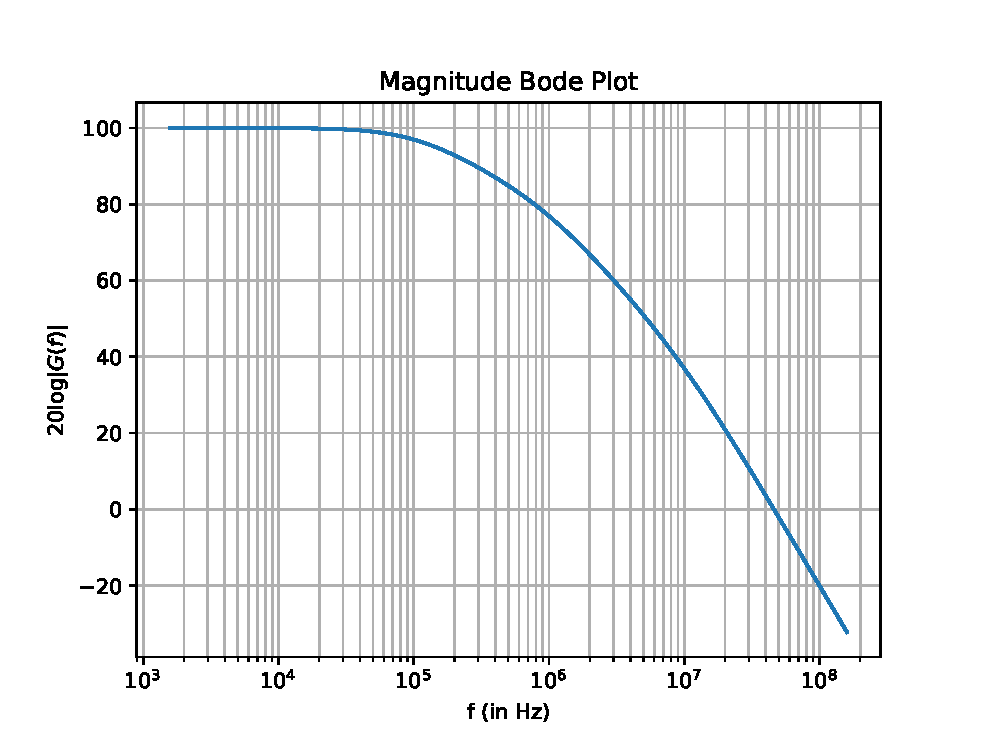
\includegraphics[width=\columnwidth]{./figs/ee18btech11014/Magnitude_Plot.eps}
	\end{center}
	\caption{Magnitude Bode Plot}
	\label{fig:Magnitude Plot}
\end{figure}

Phase Plot is \ref{fig:Phase Plot}
\begin{figure}[ht!]
	\begin{center}
		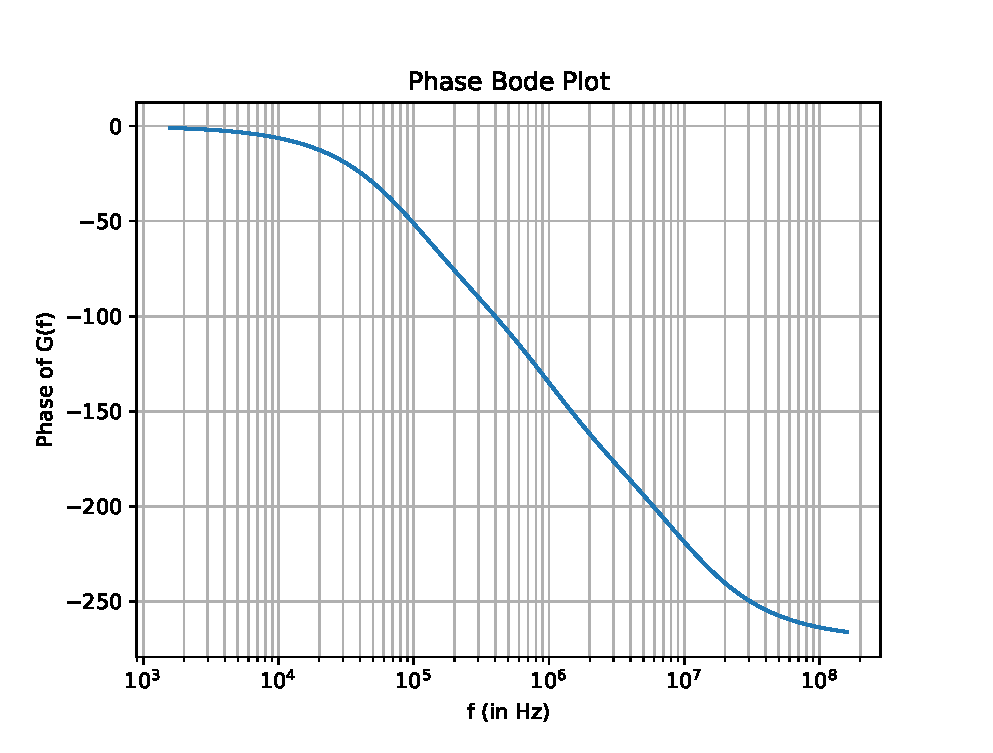
\includegraphics[width=\columnwidth]{./figs/ee18btech11014/Phase_Plot.eps}
	\end{center}
	\caption{Phase Bode Plot}
	\label{fig:Phase Plot}
\end{figure}

Python Code for Magnitude and Phase Bode Plots is at
\begin{lstlisting}
codes/ee18btech11014/Bode_Plot.py
\end{lstlisting}

%-------------------------------------------------------------------------------------------------%
%2.1.13
\item  Design a Closed-Loop Transfer Function by combining both the Open-Loop and Feedback Circuits. Also draw its Equivalent Circuit\\
\solution\\
The Closed-Loop Circuit is
\begin{figure}[ht!]
	\begin{center}
		\resizebox{\columnwidth}{!}{\begin{circuitikz}[american]

\draw (2,2)  node[op amp] (OA) {};
\draw (OA.up) -- ++(0, 0.3) node[vcc]{$+10V$};
\draw (OA.down) -- ++(0,-0.3) node[vee]{$-10V$};
\draw (OA.+) -- (0,1.5) to[vsourcesin, l= $v_{s}$] (0,0) node[ground](GND){};
\draw (OA.-) -- (0,2.5) to[R=$10\ohm$] (-2,2.5) node[ground, rotate=270](GND){};
\draw (OA.out) -- (3,2) node[label={below:$v_{a}$}]{};
\draw (3,2) to[R=$10^{2}\ohm$] (5.5,2) node[label={above:$v_{b}$}]{} to[C,l_=$\frac{10^{-9}}{2\pi}F$] (5.5,0) node[ground](GND){};
\draw (5.5,2) to[R=$10^{3}\ohm$] (8,2) node[label={above:$v_{c}$}]{} to[C,l_=$\frac{10^{-9}}{2\pi}F$] (8,0) node[ground](GND){};
\draw (8,2) to[R=$10^{4}\ohm$] (10.5,2) to[C,l_=$\frac{10^{-9}}{2\pi}F$] (10.5,0) node[ground](GND){};
\draw (10.5,2) -- (11.5,2) node[label={above:$v_{o}$}]{};
\draw (10.5,2) -- (10.5,4) to[R=$1.778\times 10^{5}\ohm$] (0,4) -- (0,2.5);

\end{circuitikz}
}
	\end{center}
	\caption{}
	\label{fig:ee18btech11014_Closed-Loop Circuit}
\end{figure}

The Equivalent Circuit of Closed-Loop Circuit is
\begin{figure}[ht!]
	\begin{center}
		\resizebox{\columnwidth}{!}{\begin{circuitikz}[american]-1
\draw (-3,0) node[ground](GND){} to[vsourcesin, l= $v_{s}$] (-3,2) to[short,-o] (0.25,2) node[label={below:$+$}]{};
\draw (0,0.1) to[R=$10\ohm$,v=$v_{f}$] (-2,0.1) node[ground](GND){}; 
\draw (0,0.1) -- (1,0.1) -- (1,4) to[R=$1.778\times 10^{5}\ohm$] (10.5,4) -- (10.5,2);


\draw (0.25,0.1) to[short,-o] (0.25,0.1) node[label={above:$-$}]{};
\draw (0.25,0.625) node[label={$v_{i}$}] {};


\draw (3,2) node[label={above:$v_{a}$}]{};
\draw (3,0) node[ground](GND){} to[vsourcesin, l= $10^5 v_{i}$] (3,2);
\draw (3,2) to[R=$10^{2}\ohm$] (5.5,2) node[label={above:$v_{b}$}]{} to[C,l_=$\frac{10^{-9}}{2\pi}F$] (5.5,0) node[ground](GND){};
\draw (5.5,2) to[R=$10^{3}\ohm$] (8,2) node[label={above:$v_{c}$}]{} to[C,l_=$\frac{10^{-9}}{2\pi}F$] (8,0) node[ground](GND){};
\draw (8,2) to[R=$10^{4}\ohm$] (10.5,2) to[C,l_=$\frac{10^{-9}}{2\pi}F$] (10.5,0) node[ground](GND){};
\draw (10.5,2) -- (11.5,2) node[label={above:$v_{o}$}]{};

\end{circuitikz}
}
	\end{center},
	\caption{}
	\label{fig:ee18btech11014_Closed-Loop Equivalent Circuit}
\end{figure}

From the Equivalent Circuit Diagram,
\begin{align}
G = \frac{v_{o}}{v_{i}} = \dfrac{10^5}{\left(1+j\frac{f}{10^{5}}\right)\left(1+j\frac{f}{10^{6}}\right)\left(1+j\frac{f}{10^{7}}\right)}\\
H = \frac{v_{f}}{v_{o}} = 5.623 \times 10^{-5}
\end{align}

The Closed-Loop Gain,
\begin{align}
v_{i} = v_{s} - v_{f}\\
\frac{v_{o}}{G} = v_{s} - Hv_{o}\\
\frac{v_{o}}{v_{s}} = \frac{G}{1+GH}
\end{align}

So, the Closed-Loop Gain,
\begin{align}
T = \frac{v_{o}}{v_{s}} = \dfrac{10^5}{5.623 + \left(1+j\frac{f}{10^{5}}\right)\left(1+j\frac{f}{10^{6}}\right)\left(1+j\frac{f}{10^{7}}\right)}
\end{align}

\end{enumerate}

\subsection{Marginal Stability}
\begin{enumerate}[label=\thesubsection.\arabic*.,ref=\thesubsection.\theenumi]
\numberwithin{equation}{enumi}

\item Fig. \ref{fig:ee18btech11005_original_circuit} shows a  non-inverting op-amp configuration   with parameters described in Table \ref{table:ee18btech11005_Input_Table}.  Draw the equivalent control system.
\renewcommand{\thefigure}{\theenumi.\arabic{figure}}
%
\begin{figure}[!ht]
	\begin{center}
		
		\resizebox{\columnwidth}{!}{\begin{circuitikz}
\ctikzset{bipoles/length=1cm}

\draw 
(0, 0) node[op amp] (opamp) {}
(opamp.-) to[R,l_=$R_1$,*-*] (-2, 0.35) to (-2.5, 0.35) to (-2.5, 0.35) node[ground]{}
(opamp.-) --(-0.9,1) to[R=$R_2$] (1,1) -- (1,0) --(2,0) node at(2.3,0){$V_0$}
(opamp.out) to (1.5,0)--(1.5,-0.5) to[R=$R_L$] (1.5,-1.5) to (1.5,-1.5) node[ground]{}
(opamp.+) -- (-0.6,-0.35) to[R =$R_s$,*-*] (-2.6,-0.35) to[V=$V_s$] (-2.6,-2.4) node[ground]{}
;\end{circuitikz}
}
	\end{center}
\caption{}
\label{fig:ee18btech11005_original_circuit}
\end{figure}
%
\begin{table}[!ht]
\centering

%%%%%%%%%%%%%%%%%%%%%%%%%%%%%%%%%%%%%%%%%%%%%%%%%%%%%%%%%%%%%%%%%%%%%%
%%                                                                  %%
%%  This is the header of a LaTeX2e file exported from Gnumeric.    %%
%%                                                                  %%
%%  This file can be compiled as it stands or included in another   %%
%%  LaTeX document. The table is based on the longtable package so  %%
%%  the longtable options (headers, footers...) can be set in the   %%
%%  preamble section below (see PRAMBLE).                           %%
%%                                                                  %%
%%  To include the file in another, the following two lines must be %%
%%  in the including file:                                          %%
%%        \def\inputGnumericTable{}                                 %%
%%  at the beginning of the file and:                               %%
%%        \input{name-of-this-file.tex}                             %%
%%  where the table is to be placed. Note also that the including   %%
%%  file must use the following packages for the table to be        %%
%%  rendered correctly:                                             %%
%%    \usepackage[latin1]{inputenc}                                 %%
%%    \usepackage{color}                                            %%
%%    \usepackage{array}                                            %%
%%    \usepackage{longtable}                                        %%
%%    \usepackage{calc}                                             %%
%%    \usepackage{multirow}                                         %%
%%    \usepackage{hhline}                                           %%
%%    \usepackage{ifthen}                                           %%
%%  optionally (for landscape tables embedded in another document): %%
%%    \usepackage{lscape}                                           %%
%%                                                                  %%
%%%%%%%%%%%%%%%%%%%%%%%%%%%%%%%%%%%%%%%%%%%%%%%%%%%%%%%%%%%%%%%%%%%%%%



%%  This section checks if we are begin input into another file or  %%
%%  the file will be compiled alone. First use a macro taken from   %%
%%  the TeXbook ex 7.7 (suggestion of Han-Wen Nienhuys).            %%
\def\ifundefined#1{\expandafter\ifx\csname#1\endcsname\relax}


%%  Check for the \def token for inputed files. If it is not        %%
%%  defined, the file will be processed as a standalone and the     %%
%%  preamble will be used.                                          %%
\ifundefined{inputGnumericTable}

%%  We must be able to close or not the document at the end.        %%
	\def\gnumericTableEnd{\end{document}}


%%%%%%%%%%%%%%%%%%%%%%%%%%%%%%%%%%%%%%%%%%%%%%%%%%%%%%%%%%%%%%%%%%%%%%
%%                                                                  %%
%%  This is the PREAMBLE. Change these values to get the right      %%
%%  paper size and other niceties.                                  %%
%%                                                                  %%
%%%%%%%%%%%%%%%%%%%%%%%%%%%%%%%%%%%%%%%%%%%%%%%%%%%%%%%%%%%%%%%%%%%%%%

	\documentclass[12pt%
			  %,landscape%
                    ]{report}
       \usepackage[latin1]{inputenc}
       \usepackage{fullpage}
       \usepackage{color}
       \usepackage{array}
       \usepackage{longtable}
       \usepackage{calc}
       \usepackage{multirow}
       \usepackage{hhline}
       \usepackage{ifthen}



%%  End of the preamble for the standalone. The next section is for %%
%%  documents which are included into other LaTeX2e files.          %%
\else

%%  We are not a stand alone document. For a regular table, we will %%
%%  have no preamble and only define the closing to mean nothing.   %%
    \def\gnumericTableEnd{}

%%  If we want landscape mode in an embedded document, comment out  %%
%%  the line above and uncomment the two below. The table will      %%
%%  begin on a new page and run in landscape mode.                  %%
%       \def\gnumericTableEnd{\end{landscape}}
%       \begin{landscape}


%%  End of the else clause for this file being \input.              %%
\fi

%%%%%%%%%%%%%%%%%%%%%%%%%%%%%%%%%%%%%%%%%%%%%%%%%%%%%%%%%%%%%%%%%%%%%%
%%                                                                  %%
%%  The rest is the gnumeric table, except for the closing          %%
%%  statement. Changes below will alter the table's appearance.     %%
%%                                                                  %%
%%%%%%%%%%%%%%%%%%%%%%%%%%%%%%%%%%%%%%%%%%%%%%%%%%%%%%%%%%%%%%%%%%%%%%

\providecommand{\gnumericmathit}[1]{#1} 
%%  Uncomment the next line if you would like your numbers to be in %%
%%  italics if they are italizised in the gnumeric table.           %%
%\renewcommand{\gnumericmathit}[1]{\mathit{#1}}
\providecommand{\gnumericPB}[1]%
{\let\gnumericTemp=\\#1\let\\=\gnumericTemp\hspace{0pt}}
 \ifundefined{gnumericTableWidthDefined}
        \newlength{\gnumericTableWidth}
        \newlength{\gnumericTableWidthComplete}
        \newlength{\gnumericMultiRowLength}
        \global\def\gnumericTableWidthDefined{}
 \fi
%% The following setting protects this code from babel shorthands.  %%
 \ifthenelse{\isundefined{\languageshorthands}}{}{\languageshorthands{english}}
%%  The default table format retains the relative column widths of  %%
%%  gnumeric. They can easily be changed to c, r or l. In that case %%
%%  you may want to comment out the next line and uncomment the one %%
%%  thereafter                                                      %%
\providecommand\gnumbox{\makebox[0pt]}
%%\providecommand\gnumbox[1][]{\makebox}

%% to adjust positions in multirow situations                       %%
\setlength{\bigstrutjot}{\jot}
\setlength{\extrarowheight}{\doublerulesep}

%%  The \setlongtables command keeps column widths the same across  %%
%%  pages. Simply comment out next line for varying column widths.  %%
\setlongtables

\setlength\gnumericTableWidth{%
	53pt+%
	93pt+%
0pt}
\def\gumericNumCols{2}
\setlength\gnumericTableWidthComplete{\gnumericTableWidth+%
         \tabcolsep*\gumericNumCols*2+\arrayrulewidth*\gumericNumCols}
\ifthenelse{\lengthtest{\gnumericTableWidthComplete > \linewidth}}%
         {\def\gnumericScale{\ratio{\linewidth-%
                        \tabcolsep*\gumericNumCols*2-%
                        \arrayrulewidth*\gumericNumCols}%
{\gnumericTableWidth}}}%
{\def\gnumericScale{1}}

%%%%%%%%%%%%%%%%%%%%%%%%%%%%%%%%%%%%%%%%%%%%%%%%%%%%%%%%%%%%%%%%%%%%%%
%%                                                                  %%
%% The following are the widths of the various columns. We are      %%
%% defining them here because then they are easier to change.       %%
%% Depending on the cell formats we may use them more than once.    %%
%%                                                                  %%
%%%%%%%%%%%%%%%%%%%%%%%%%%%%%%%%%%%%%%%%%%%%%%%%%%%%%%%%%%%%%%%%%%%%%%

\ifthenelse{\isundefined{\gnumericColA}}{\newlength{\gnumericColA}}{}\settowidth{\gnumericColA}{\begin{tabular}{@{}p{110pt*\gnumericScale}@{}}x\end{tabular}}
\ifthenelse{\isundefined{\gnumericColB}}{\newlength{\gnumericColB}}{}\settowidth{\gnumericColB}{\begin{tabular}{@{}p{20pt*\gnumericScale}@{}}x\end{tabular}}

\begin{tabular}[c]{%
	b{\gnumericColA}%
	b{\gnumericColB}%
	}

%%%%%%%%%%%%%%%%%%%%%%%%%%%%%%%%%%%%%%%%%%%%%%%%%%%%%%%%%%%%%%%%%%%%%%
%%  The longtable options. (Caption, headers... see Goosens, p.124) %%
%	\caption{The Table Caption.}             \\	%
% \hline	% Across the top of the table.
%%  The rest of these options are table rows which are placed on    %%
%%  the first, last or every page. Use \multicolumn if you want.    %%

%%  Header for the first page.                                      %%
%	\multicolumn{2}{c}{The First Header} \\ \hline 
%	\multicolumn{1}{c}{colTag}	%Column 1
%	&\multicolumn{1}{c}{colTag}	\\ \hline %Last column
%	\endfirsthead

%%  The running header definition.                                  %%
%	\hline
%	\multicolumn{2}{l}{\ldots\small\slshape continued} \\ \hline
%	\multicolumn{1}{c}{colTag}	%Column 1
%	&\multicolumn{1}{c}{colTag}	\\ \hline %Last column
%	\endhead

%%  The running footer definition.                                  %%
%	\hline
%	\multicolumn{2}{r}{\small\slshape continued\ldots} \\
%	\endfoot

%%  The ending footer definition.                                   %%
%	\multicolumn{2}{c}{That's all folks} \\ \hline 
%	\endlastfoot
%%%%%%%%%%%%%%%%%%%%%%%%%%%%%%%%%%%%%%%%%%%%%%%%%%%%%%%%%%%%%%%%%%%%%%

\hhline{|-|-}
	 \multicolumn{1}{|p{\gnumericColA}|}%
	{\gnumericPB{\centering}\gnumbox{\textbf{Parameter}}}
	&\multicolumn{1}{p{\gnumericColB}|}%
	{\gnumericPB{\centering}\gnumbox{\textbf{Value}}}
\\
\hhline{|-|-}
	 \multicolumn{1}{|p{\gnumericColA}|}%
	{\gnumericPB{\centering}\gnumbox{\textbf{input resistance}}}
	&\multicolumn{1}{p{\gnumericColB}|}%
	{\gnumericPB{\centering}\gnumbox{\textbf{$\infty$}}}
\\
\hhline{|-|-}
	 \multicolumn{1}{|p{\gnumericColA}|}%
	{\gnumericPB{\centering}\gnumbox{\textbf{output resistance}}}
	&\multicolumn{1}{p{\gnumericColB}|}%
	{\gnumericPB{\centering}\gnumbox{\textbf{0}}}
\\
\hhline{|-|-}
	 \multicolumn{1}{|p{\gnumericColA}|}%
	{\gnumericPB{\centering}\gnumbox{\textbf{Input voltage}}}
	&\multicolumn{1}{p{\gnumericColB}|}%
	{\gnumericPB{\centering}\gnumbox{\textbf{$V_s$}}}
\\
\hhline{|-|-}
	 \multicolumn{1}{|p{\gnumericColA}|}%
	{\gnumericPB{\centering}\gnumbox{\textbf{Output Voltage}}}
	&\multicolumn{1}{p{\gnumericColB}|}%
	{\gnumericPB{\centering}\gnumbox{\textbf{$V_o$}}}
\\
\hhline{|-|-}
	 \multicolumn{1}{|p{\gnumericColA}|}%
	{\gnumericPB{\centering}\gnumbox{\textbf{Feeding resistance}}}
	&\multicolumn{1}{p{\gnumericColB}|}%
	{\gnumericPB{\centering}\gnumbox{\textbf{$R_1$}}}
\\

\hhline{|-|-}
	 \multicolumn{1}{|p{\gnumericColA}|}%
	{\gnumericPB{\centering}\gnumbox{\textbf{Feedback resistance}}}
	&\multicolumn{1}{p{\gnumericColB}|}%
	{\gnumericPB{\centering}\gnumbox{\textbf{$R_2$}}}
\\
\hhline{|-|-}
	 \multicolumn{1}{|p{\gnumericColA}|}%
	{\gnumericPB{\centering}\gnumbox{\textbf{Source resistance}}}
	&\multicolumn{1}{p{\gnumericColB}|}%
	{\gnumericPB{\centering}\gnumbox{\textbf{$R_s$}}}
\\
\hhline{|-|-}
	 \multicolumn{1}{|p{\gnumericColA}|}%
	{\gnumericPB{\centering}\gnumbox{\textbf{load resistance}}}
	&\multicolumn{1}{p{\gnumericColB}|}%
	{\gnumericPB{\centering}\gnumbox{\textbf{$R_L$}}}
\\

\hhline{|-|-|}
\end{tabular}

\ifthenelse{\isundefined{\languageshorthands}}{}{\languageshorthands{\languagename}}
\gnumericTableEnd

\caption{}
\label{table:ee18btech11005_Input_Table}
\end{table}
\\
\solution  See 	Fig. \ref{fig:ee18btech11005_equivalent_control_system}
\begin{figure}[!ht]
	\begin{center}
			\resizebox{\columnwidth}{!}{
\tikzstyle{block} = [draw, fill=blue!20, rectangle, 
    minimum height=3em, minimum width=6em]
\tikzstyle{sum} = [draw, fill=blue!20, circle, node distance=1cm]
\tikzstyle{input} = [coordinate]
\tikzstyle{output} = [coordinate]
\tikzstyle{pinstyle} = [pin edge={to-,thin,black}]

\begin{tikzpicture}[auto, node distance=2cm,>=latex']
    \node [input, name=input] {$V_s$};
    \node [sum, right of=input] (sum) {};
    \node [block, right of=sum] (controller) {$G$};
    \node [output, right of=controller] (output) {};
    \node [block, below of=controller] (feedback) {$H$};
    \draw [draw,->] (input) -- node {$V_s$} (sum);
    \draw [->] (sum) -- node {$V_i$} (controller);
    \draw [->] (controller) -- node [name=y] {$V_o$}(output);
    \draw [->] (y) |- (feedback);
    \draw [->] (feedback) -| node[pos=0.99]{$-$}  node [near end] {$V_f$} (sum);
\end{tikzpicture}
}
	\end{center}
\caption{}
\label{fig:ee18btech11005_equivalent_control_system}
\end{figure}
\renewcommand{\thefigure}{\theenumi}

\item Draw the small signal model for Fig. \ref{fig:ee18btech11005_original_circuit}.
\\
\solution
The equivalent circuit of the amplifier is in Fig. \ref{fig:ee18btech11005_equivalent_circuit}
\begin{figure}[!ht]
	\begin{center}
		
		\resizebox{\columnwidth}{!}{\usetikzlibrary{decorations.markings}
\begin{circuitikz}
\ctikzset{bipoles/length=1cm}

\draw 
(0, 0) to[V=$V_s$] (0,-1.5) to (0,-1.5) node[ground]{}
(0,0) -- (0,1)--(0.25,1) to[R=$R_s$] (1.5,1)  node at(1.8,1){$+$}
%(1.5,3) node[pos=10]{$V_i$}
(1.5,-1.25)  node at(1.7,-1.25){$-$} 
(1.5,-1.25) -- (1,-1.25) -- (1,-1.75) to[R=$R_1$] (1,-2.75) --(1,-3) node[ground]{}
(1,-1.5) to[R=$R_2$] (5,-1.5){}
(5,-1.5) -- (5,1) --(3.5,1) to[V=$GV_i$] (3.5,-0.5) node[ground]{}
(5,1) --(6,1) to[R=$R_l$,*-*] (6,-0.5) node[ground]{}
(6,1) --(6.5,1) node at(6.8,1){$V_0$}
node at(1.8,-0.3) {$V_i$}
node at(0.6,-1.75){$+$}
node at(0.6,-3){$-$}
node at(0.6,-2.5){$V_f$}
;\end{circuitikz}
}
	\end{center}
\caption{}
\label{fig:ee18btech11005_equivalent_circuit}
\end{figure}

\item Assuming that the operational amplifier has infinite input resistance and zero output resistance, find  the {\em feedback factor} $H$.
\\
\solution From Fig. \ref{fig:ee18btech11005_equivalent_circuit},

\begin{align}
\label{eq:ee18btech11005_opamp_output}
V_0 &= GV_i
\\
 V_i &= V_s -V_f
\\
V_f &= \frac{R_1}{R_1+R_2}V_o
\end{align}
%
assuming that the current through $R_s$ is very small.  Thus, 
\begin{align}
H &=  \frac{V_f}{V_o} = \frac{R_1}{R_1+R_2}
\label{eq:ee18btech11005_H}
\end{align}
\item  Obtain the closed loop gain $T$ and summarize your results through a Table.
\\
\solution Table \ref{table:ee18btech11005_Output_Table} provides a summary.

\begin{align}
\label{eq:ee18btech11005_T}
T &=    \frac{V_0}{V_i}= \frac{G}{1+GH}
  \\
&= \frac{G\brak{R_1+R_2}}{\brak{R_1+R_2}+GR_1}
\end{align}
\begin{table}[!ht]
\centering


%%  This section checks if we are begin input into another file or  %%
%%  the file will be compiled alone. First use a macro taken from   %%
%%  the TeXbook ex 7.7 (suggestion of Han-Wen Nienhuys).            %%
\def\ifundefined#1{\expandafter\ifx\csname#1\endcsname\relax}


%%  Check for the \def token for inputed files. If it is not        %%
%%  defined, the file will be processed as a standalone and the     %%
%%  preamble will be used.                                          %%
\ifundefined{inputGnumericTable}

%%  We must be able to close or not the document at the end.        %%
	\def\gnumericTableEnd{\end{document}}


%%%%%%%%%%%%%%%%%%%%%%%%%%%%%%%%%%%%%%%%%%%%%%%%%%%%%%%%%%%%%%%%%%%%%%
%%                                                                  %%
%%  This is the PREAMBLE. Change these values to get the right      %%
%%  paper size and other niceties.                                  %%
%%                                                                  %%
%%%%%%%%%%%%%%%%%%%%%%%%%%%%%%%%%%%%%%%%%%%%%%%%%%%%%%%%%%%%%%%%%%%%%%

	\documentclass[12pt%
			  %,landscape%
                    ]{report}
       \usepackage[latin1]{inputenc}
       \usepackage{fullpage}
       \usepackage{color}
       \usepackage{array}
       \usepackage{longtable}
       \usepackage{calc}
       \usepackage{multirow}
       \usepackage{hhline}
       \usepackage{ifthen}
%%  End of the preamble for the standalone. The next section is for %%
%%  documents which are included into other LaTeX2e files.          %%
\else

%%  We are not a stand alone document. For a regular table, we will %%
%%  have no preamble and only define the closing to mean nothing.   %%
    \def\gnumericTableEnd{}

%%  If we want landscape mode in an embedded document, comment out  %%
%%  the line above and uncomment the two below. The table will      %%
%%  begin on a new page and run in landscape mode.                  %%
%       \def\gnumericTableEnd{\end{landscape}}
%       \begin{landscape}


%%  End of the else clause for this file being \input.              %%
\fi

%%%%%%%%%%%%%%%%%%%%%%%%%%%%%%%%%%%%%%%%%%%%%%%%%%%%%%%%%%%%%%%%%%%%%%
%%                                                                  %%
%%  The rest is the gnumeric table, except for the closing          %%
%%  statement. Changes below will alter the table's appearance.     %%
%%                                                                  %%
%%%%%%%%%%%%%%%%%%%%%%%%%%%%%%%%%%%%%%%%%%%%%%%%%%%%%%%%%%%%%%%%%%%%%%

\providecommand{\gnumericmathit}[1]{#1} 
%%  Uncomment the next line if you would like your numbers to be in %%
%%  italics if they are italizised in the gnumeric table.           %%
%\renewcommand{\gnumericmathit}[1]{\mathit{#1}}
\providecommand{\gnumericPB}[1]%
{\let\gnumericTemp=\\#1\let\\=\gnumericTemp\hspace{0pt}}
 \ifundefined{gnumericTableWidthDefined}
        \newlength{\gnumericTableWidth}
        \newlength{\gnumericTableWidthComplete}
        \newlength{\gnumericMultiRowLength}
        \global\def\gnumericTableWidthDefined{}
 \fi
%% The following setting protects this code from babel shorthands.  %%
 \ifthenelse{\isundefined{\languageshorthands}}{}{\languageshorthands{english}}
%%  The default table format retains the relative column widths of  %%
%%  gnumeric. They can easily be changed to c, r or l. In that case %%
%%  you may want to comment out the next line and uncomment the one %%
%%  thereafter                                                      %%
\providecommand\gnumbox{\makebox[0pt]}
%%\providecommand\gnumbox[1][]{\makebox}

%% to adjust positions in multirow situations                       %%
\setlength{\bigstrutjot}{\jot}
\setlength{\extrarowheight}{\doublerulesep}

%%  The \setlongtables command keeps column widths the same across  %%
%%  pages. Simply comment out next line for varying column widths.  %%
\setlongtables

\setlength\gnumericTableWidth{%
	50pt+%
	50pt+%
	50pt+%
0pt}
\def\gumericNumCols{3}
\setlength\gnumericTableWidthComplete{\gnumericTableWidth+%
         \tabcolsep*\gumericNumCols*2+\arrayrulewidth*\gumericNumCols}
\ifthenelse{\lengthtest{\gnumericTableWidthComplete > \linewidth}}%
         {\def\gnumericScale{\ratio{\linewidth-%
                        \tabcolsep*\gumericNumCols*2-%
                        \arrayrulewidth*\gumericNumCols}%
{\gnumericTableWidth}}}%
{\def\gnumericScale{1}}

%%%%%%%%%%%%%%%%%%%%%%%%%%%%%%%%%%%%%%%%%%%%%%%%%%%%%%%%%%%%%%%%%%%%%%
%%                                                                  %%
%% The following are the widths of the various columns. We are      %%
%% defining them here because then they are easier to change.       %%
%% Depending on the cell formats we may use them more than once.    %%
%%                                                                  %%
%%%%%%%%%%%%%%%%%%%%%%%%%%%%%%%%%%%%%%%%%%%%%%%%%%%%%%%%%%%%%%%%%%%%%%

\ifthenelse{\isundefined{\gnumericColA}}{\newlength{\gnumericColA}}{}\settowidth{\gnumericColA}{\begin{tabular}{@{}p{50pt*\gnumericScale}@{}}x\end{tabular}}
\ifthenelse{\isundefined{\gnumericColB}}{\newlength{\gnumericColB}}{}\settowidth{\gnumericColB}{\begin{tabular}{@{}p{60pt*\gnumericScale}@{}}x\end{tabular}}
\ifthenelse{\isundefined{\gnumericColC}}{\newlength{\gnumericColC}}{}\settowidth{\gnumericColC}{\begin{tabular}{@{}p{60pt*\gnumericScale}@{}}x\end{tabular}}

\begin{tabular}[c]{%
	b{\gnumericColA}%
	b{\gnumericColB}%
	b{\gnumericColC}%
	}

%%%%%%%%%%%%%%%%%%%%%%%%%%%%%%%%%%%%%%%%%%%%%%%%%%%%%%%%%%%%%%%%%%%%%%
%%  The longtable options. (Caption, headers... see Goosens, p.124) %%
%	\caption{The Table Caption.}             \\	%
% \hline	% Across the top of the table.
%%  The rest of these options are table rows which are placed on    %%
%%  the first, last or every page. Use \multicolumn if you want.    %%

%%  Header for the first page.                                      %%
%	\multicolumn{3}{c}{The First Header} \\ \hline 
%	\multicolumn{1}{c}{colTag}	%Column 1
%	&\multicolumn{1}{c}{colTag}	%Column 2
%	&\multicolumn{1}{c}{colTag}	\\ \hline %Last column
%	\endfirsthead

%%  The running header definition.                                  %%
%	\hline
%	\multicolumn{3}{l}{\ldots\small\slshape continued} \\ \hline
%	\multicolumn{1}{c}{colTag}	%Column 1
%	&\multicolumn{1}{c}{colTag}	%Column 2
%	&\multicolumn{1}{c}{colTag}	\\ \hline %Last column
%	\endhead

%%  The running footer definition.                                  %%
%	\hline
%	\multicolumn{3}{r}{\small\slshape continued\ldots} \\
%	\endfoot

%%  The ending footer definition.                                   %%
%	\multicolumn{3}{c}{That's all folks} \\ \hline 
%	\endlastfoot
%%%%%%%%%%%%%%%%%%%%%%%%%%%%%%%%%%%%%%%%%%%%%%%%%%%%%%%%%%%%%%%%%%%%%%

\hhline{|-|-|-}
	 \multicolumn{1}{|p{\gnumericColA}|}%
	{\gnumericPB{\centering}\textbf{Parameters}}
	&\multicolumn{1}{p{\gnumericColB}|}%
	{\gnumericPB{\centering}\textbf{Definition}}
	&\multicolumn{1}{p{\gnumericColC}|}%
	{\gnumericPB{\centering}\textbf{For given circuit}}

	
\\


\hhline{|---|}
	 \multicolumn{1}{|p{\gnumericColA}|}%
	{\gnumericPB{\centering}{Open loop gain}}
	&\multicolumn{1}{p{\gnumericColB}|}%
	{\gnumericPB{\centering}G}
	&\multicolumn{1}{p{\gnumericColC}|}%
	{\gnumericPB{\centering}G}

\\
\hhline{|---|}
	 \multicolumn{1}{|p{\gnumericColA}|}%
	{\gnumericPB{\centering}Feedback factor}
	&\multicolumn{1}{p{\gnumericColB}|}%
	{\gnumericPB{\centering}H}
	&\multicolumn{1}{p{\gnumericColC}|}%
	{\gnumericPB{\centering}{$\frac{R_1}{R_1+R_2}$}}

\\
\hhline{|---|}
	 \multicolumn{1}{|p{\gnumericColA}|}%
	{\gnumericPB{\centering}Loop gain}
	&\multicolumn{1}{p{\gnumericColB}|}%
	{\gnumericPB{\centering}GH}
	&\multicolumn{1}{p{\gnumericColC}|}%
	{\gnumericPB{\centering}{$G\frac{R_1}{R_1+R_2}$}}

\\


\hhline{|-|-|-|}
    \multicolumn{1}{|p{\gnumericColA}|}%
	{\gnumericPB{\centering}Amount of feedback}
	&\multicolumn{1}{p{\gnumericColB}|}%
	{\gnumericPB{\centering}1+GH}
	&\multicolumn{1}{p{\gnumericColC}|}%
	{\gnumericPB{\centering}{$1+\frac{GR_1}{R_1+R_2}$}}

\\
\hhline{|---|}
	 \multicolumn{1}{|p{\gnumericColA}|}%
	{\gnumericPB{\centering}Closed loop gain }
	&\multicolumn{1}{p{\gnumericColB}|}%
	{\gnumericPB{\centering}{$\frac{G}{1+GH}$}}
	&\multicolumn{1}{p{\gnumericColC}|}%
	{\gnumericPB{\centering}{$\frac{G(R_1+R_2)}{R_1+R_2+GR_1}$}}

\\
\hhline{|-|-|-|}
\end{tabular}

\ifthenelse{\isundefined{\languageshorthands}}{}{\languageshorthands{\languagename}}
\gnumericTableEnd

\caption{}
\label{table:ee18btech11005_Output_Table}
\end{table}
%
\item Find the condition under which closed loop gain T is almost entirely determined by the feedback network.
\\
\solution If 

\begin{align}
 GH &\gg 1,
 \\
T &\approx \frac{1}{H}  = 1 + \frac{R_2}{R_1} 
\label{eq:ee18btech11005_T}
\end{align}
\item If 
\begin{align} 
G & = 10^4
\\
T &= 10,
\end{align}
find $H$.
%$\frac{R_2}{R_1}$.
\\
\solution From Table \ref{table:ee18btech11005_Output_Table}
\begin{align}
    T &=  \frac{G}{1+GH} = 10
\\
\implies  H &= 0.0999
%\frac{R_2}{R_1} &= 9.010
\end{align}
%\item What is the amount of feedback in decibels?
%\solution The value of F in decibals is given by 
%\begin{align}
%    F(dB) &= 20\log\brak{1+GH}\\
%F(dB) &= 60 dB
%\end{align}
\item {\em Gain Desensitivity:} If G decreases by 20\%,what is the corresponding decrease in T?  Comment.
\\
\solution From From Table \ref{table:ee18btech11005_Output_Table},
Given
\begin{align}
T &= \frac{G}{1+GH}
\\
\implies dT &= \frac{dG}{\brak{1+GH}^2}
\\
\implies \frac{dT}{T} &= \frac{1}{1+GH}\frac{dG}{G}
\end{align}
From the information available so far, 
\begin{align}
dG = 20\%, G = 10^4, H = 0.0999
\implies \frac{dT}{T} = 0.025\%
\end{align}
%
using the following code.
\begin{lstlisting}
codes/ee18btech11005/ee18btech11005.py
\end{lstlisting}
%
Thus the closed loop gain is almost invariant to a relatively large (20\%) variation in the open loop gain $G$.  This is known as gain desensitivity.
\end{enumerate}

\subsection{Stability}
\begin{enumerate}[label=\thesubsection.\arabic*.,ref=\thesubsection.\theenumi]
\numberwithin{equation}{enumi}
\item 
The characteristic equation of linear time invariant system is given by
\begin{align} 
\nabla(s)=s^4+3s^3+3s^2+s+k=0
\end{align}
Find the condition for the system to be BIBO stable using the Routh Array.

\textbf{solution}
\begin{align}
\nabla(s)=s^4+3s^3+3s^2+s+k=0
\end{align}

The Routh hurwitz criterion:-
\bigskip
\begin{align}
\mydet{s^4\\s^3\\s^2\\s^1 \\ s^0}
\mydet{1 & 3 & k \\ 3 & 1 & 0\\  \frac{8}{3}& k & 0\\ \frac{\frac{8}{3}-3k}{\frac{8}{3}} & 0 & 0\\k & 0 & 0} 
\end{align}
From the above array, the given system is stable if
\begin{align}
\begin{split}
k&>0 
\\
  \frac{\frac{8}{3}-3k}{\frac{8}{3}}&>0    
\end{split}
\\
\implies 0<k<\frac{8}{9}
\end{align}
%
\item Modify the Python code in Problem \ref{prob:ee18btech11005_python} to verify your solution by choosing two different values of $k$.
\label{prob:ee18btech11008_python}
\\
\solution 
The following code 
%
\begin{lstlisting}
codes/ee18btech11008.py
\end{lstlisting}
%
provides the necessary soution for $k = 0.5, 3$.
\begin{itemize}
  \item $k=0.5 < \frac{8}{9}$ has no sign changes in first column of its routh array.So the system is stable.
  \item $k=3 > \frac{8}{9}$ has 2 sign changes in first column of its routh array.So the system is unstable.
  \end{itemize}

\end{enumerate}

\subsection{Example}
\begin{enumerate}[label=\thesubsection.\arabic*.,ref=\thesubsection.\theenumi]
\numberwithin{equation}{enumi}

\item Consider a standard control system with negative feedback and the transfer functions 
\begin{align}
G(s) = \frac{1}{(s+1)(s+2)}
\end{align}
and
\begin{align}
H(s) = \frac{s+\alpha}{s}
\end{align}
%
Find  $\alpha$ so that 
the closed loop system has poles on the imaginary axis.
\solution The 
Characteristic equation is
\begin{align}
 1 + G(s)H(s) &= 0
\\
\implies 1 + \sbrak{\frac{1}{(s+1)(s+2)}}\sbrak{\frac{s+\alpha}{s}} &= 0
\\
\implies s^3+3s^2+3s+\alpha = 0
\label{eq:ee18btech11020_char}
\end{align}
Constructing the routh array for \eqref{eq:ee18btech11020_char},
%
\begin{align}
\mydet{s^3\\s^2}
\mydet{1 & 3 \\ 3 & \alpha }
\label{eq:sec_order_op_1}
\\
\implies \mydet{s^3\\s^2\\s^1}
\mydet{1 & 3 \\ 3 & \alpha \\  \frac{9-\alpha}{3} & 0} \label{eq:sec_order_op_1}
\\
\implies \mydet{s^3\\s^2\\s^1\\s^0}
\mydet{1 & 3 \\ 3 & \alpha \\  \frac{9-\alpha}{3} & 0\\ \alpha & 0} \label{eq:sec_order_op_1}
\end{align}
For poles on the imaginary axis any one of the rows should be zero.  Thus,
\begin{align}
\frac{9-\alpha}{3} = 0
\implies   \alpha = 9
\end{align}
Substituting $\alpha = 9$ in \eqref{eq:ee18btech11020_char},
\begin{align}
s^3+3s^2+3s+9&=0
\\
\implies s &= -3,\pm\j\sqrt{3}
\end{align}
%
verifying that poles lie on the imaginary axis.
\end{enumerate}

\section{State-Space Model}
\subsection{Controllability and Observability}
%\begin{enumerate}[label=\thesubsection.\arabic*.,ref=\thesubsection.\theenumi]
\numberwithin{equation}{enumi}
\item State the general model of a state space system specifying the dimensions of the matrices and vectors.
\\
\solution The model is given by 
\begin{align}
\label{eq:ee18btech11004_state}
\dot{\vec{x}}(t)&=\vec{A}\vec{x}(t)+\vec{B}\vec{u}(t) \\
 \vec{y}(t)&=\vec{C}\vec{x}(t)+\vec{D} \vec{u}(t)
\end{align}
%
with parameters listed in Table \ref{table:ee18btech11004}.
%
\begin{table}[!ht]
\centering
\begin{enumerate}[label=\thesubsection.\arabic*.,ref=\thesubsection.\theenumi]
\numberwithin{equation}{enumi}
\item State the general model of a state space system specifying the dimensions of the matrices and vectors.
\\
\solution The model is given by 
\begin{align}
\label{eq:ee18btech11004_state}
\dot{\vec{x}}(t)&=\vec{A}\vec{x}(t)+\vec{B}\vec{u}(t) \\
 \vec{y}(t)&=\vec{C}\vec{x}(t)+\vec{D} \vec{u}(t)
\end{align}
%
with parameters listed in Table \ref{table:ee18btech11004}.
%
\begin{table}[!ht]
\centering
\begin{enumerate}[label=\thesubsection.\arabic*.,ref=\thesubsection.\theenumi]
\numberwithin{equation}{enumi}
\item State the general model of a state space system specifying the dimensions of the matrices and vectors.
\\
\solution The model is given by 
\begin{align}
\label{eq:ee18btech11004_state}
\dot{\vec{x}}(t)&=\vec{A}\vec{x}(t)+\vec{B}\vec{u}(t) \\
 \vec{y}(t)&=\vec{C}\vec{x}(t)+\vec{D} \vec{u}(t)
\end{align}
%
with parameters listed in Table \ref{table:ee18btech11004}.
%
\begin{table}[!ht]
\centering
\input{./tables/ee18btech11004.tex}
\caption{}
\label{table:ee18btech11004}
\end{table}
\item Find the transfer function $\vec{H}(s)$ for the general system.
\\
\solution 
Taking Laplace transform on both sides we have the following equations
\begin{align}
 s\vec{IX}(s)-\vec{x}(0)&= \vec{AX}(s)+ \vec{BU}(s)\\
(s\vec{I}-\vec{A})\vec{X}(s)&= \vec{BU}(s)+ \vec{x}(0)\\
\vec{X}(s)&={(s\vec{I}-\vec{A})^{-1}}\vec{B U}(s)\\
& +(s\vec{I}-\vec{A})^{-1}\vec{x}(0)
\label{eq:x_init}
\end{align}
and
\begin{align}
\vec{Y}(s)&= \vec{CX}(s)+D\vec{IU}(s)
\end{align}
Substituting from \eqref{eq:x_init} in the above,
%
\begin{multline}
\vec{Y}(s)=( \vec{C}{(s\vec{I}-\vec{A})^{-1}}\vec{B}+D\vec{I}) \vec{U}(s) 
\\
+ \vec{C}(s\vec{I}-\vec{A})^{-1}\vec{x}(0)
\end{multline}
%
%
\item Find $H(s)$ for a SISO (single input single output) system.
\\
\solution
\begin{align}
\label{eq:ee18btech11004_siso}
H(s)= {\frac{Y(s)}{U(s)}}= C{(sI-A)^{-1}}B+DI
\end{align}

\item Given 
\begin{align}
H(s)&=\frac{1}{s^3+3s^2+2s+1}
\\
D&=0
\\
\vec{B}&= \myvec{0\\0\\1}
\end{align}
%
 find $\vec{A}$ and $\vec{C}$ such that the state-space realization is in {\em controllable canonical form}.
\\
\solution 
\begin{align} 
\because {\frac{Y(s)}{U(s)}}= \frac{Y(s)}{V(s)} \times \frac{V(s)}{U(s)},
\end{align}
letting
\begin{align}
 {\frac{Y(s)}{V(s)}}= 1, 
\end{align}
results in 
\begin{align}
{\frac{U(s)}{V(s)}}={s^3 + 3s^2+2s + 1}
\end{align}

giving
\begin{align}
U(s)= s^3 V(s) + 3s^2 V(s)+2sV(s) + V(s)
\end{align}

so equation 0.1.13 can be written as
\begin{align}
\myvec{sV(s)\\s^2V(s)\\s^3V(s)}
=
\myvec{0&1&0\\0&0&1\\-1&-2&-3}\myvec{V(s)\\s(s)\\s^2V(s)}
+
\myvec{0\\0\\1}  U
\end{align}
So 
\begin{align}
\vec{A}=\myvec{0&1&0\\0&0&1\\-1&-2&-3}
\end{align}

\begin{align}
Y=X_{1}(s)
=\myvec{1&0&0} \myvec{V(s)\\sV(s)\\s^2V(s)}
\end{align}
\begin{align}
\vec{C}=\myvec{1&0&0}
\end{align}

\item Obtain $\vec{A}$ and $\vec{C}$ so that the state-space realization in in {\em observable canonical form}.
\\
\solution  Given that
\begin{align}
H(s)&=\frac{1}{s^3+3s^2+2s+1}
\end{align}
\begin{align}
\frac{Y(s)}{U(s)}=\frac{1}{s^3+3s^2+2s+1} \\
Y(s) \times (s^3+3s^2+2s+1) = U(s)
\end{align}
\begin{align}
s^3Y(s)+3s^2Y(s)+2sY(s)+Y(s)=U(s)\\
s^3Y(s)=U(s)-3s^2Y(s)-2sY(s)-Y(s)\\
Y(s)=-3s^{-1}Y(s)-2s^{-2}Y(s)+s^{-3}(U(s)-Y(s))
\end{align}
\\ let $Y=aU+X_{1}$
\\ by comparing with equation 1.5.6 we get a=0 and
\begin{align}
Y=X_{1}
\end{align}
inverse laplace transform of above equation is 
\begin{align}
y=x_{1}
\end{align}
so from above equation 1.5.6 and 1.5.7
\begin{align}
X_{1}=-3s^{-1}Y(s)-2s^{-2}Y(s)+s^{-3}(U(s)-Y(s))\\
sX_{1}=-3Y(s)-2s^{-1}Y(s)+s^{-2}(U(s)-Y(s)) 
\end{align}
inverse laplace transform of above equation 
\begin{align}
\dot{x_{1}}=-3y+x_{2}
\end{align} 
where
\begin{align}
X_{2}=-2s^{-1}Y(s)+s^{-2}(U(s)-Y(s))\\
sX_{2}=-2Y(s)+s^{-1}(U(s)-Y(s))
\end{align} 
inverse laplace transform of above equation 
\begin{align}
\dot{x_{2}}=-2y+x_{3}
\end{align}
where
\begin{align}
X_{3}=s^{-1}(U(s)-Y(s))\\
sX_{3}=U(s)-Y(s)
\end{align} 
inverse laplace transform of above equation 
\begin{align}
\dot{x_{3}}=u-y
\end{align}
so we get four equations which are
\begin{align}
y=x_{1}\\
\dot{x_{1}}=-3y+x_{2}\\
\dot{x_{2}}=-2y+x_{3}\\
\dot{x_{3}}=u-y
\end{align} 
sub $ y=x_{1}$ in 1.5.19,1.5.20,1.5.21 we get
\begin{align}
 y=x_{1}\\
\dot{x_{1}}=-3x_{1}+x_{2}\\
\dot{x_{2}}=-2x_{1}+x_{3}\\
\dot{x_{3}}=u-x_{1}
\end{align} 
so above equations can be written as
\begin{align}
\myvec{\dot{x_{1}}\\\dot{x_{2}}\\\dot{x_{3}})}
=
\myvec{-3&1&0\\-2&0&1\\-1&0&0}\myvec{x_{1}\\x_{2}\\x_{3}}
+
\myvec{0\\0\\1}  U
\end{align}
So 
\begin{align}
\vec{A}=\myvec{-3&1&0\\-2&0&1\\-1&0&0}
\end{align}
\begin{align}
y=x_{1}
=\myvec{1&0&0} \myvec{x_{1}\\x_{2}\\x_{3}}
\end{align}
\begin{align}
\vec{C}=\myvec{1&0&0}
\end{align}


\item Find the eigenvaues of $\vec{A}$ and the poles of $H(s)$ using a python code.
\\
\solution The following code 
%
\begin{lstlisting}
codes/ee18btech11004.py
\end{lstlisting}
gives the necessary values.  The roots are the same as the eigenvalues.
%
\item Theoretically, show that eigenvaues of $\vec{A}$ are the poles of  $H(s)$.
\solution 
\\ as we know tthat  the characteristic equation is det(sI-A) 
\\\begin{align}
\vec{sI-A}=
\myvec{s&0&0\\0&s&0\\0&0&s}
-
\myvec{0&1&0\\0&0&1\\-1&-2&-3}
=\myvec{s&-1&0\\0&s&-1\\1&2&s+3}
\end{align}
\\therfore
\begin{align}
det(sI-A)=s(s^2+3s+2)+1(1)=s^3+3s^2+2s+1
\end{align} 
\\so from equation 1.6.2 we can see that charcteristic equation is equal to the denominator of the transefer function
\end{enumerate}


\caption{}
\label{table:ee18btech11004}
\end{table}
\item Find the transfer function $\vec{H}(s)$ for the general system.
\\
\solution 
Taking Laplace transform on both sides we have the following equations
\begin{align}
 s\vec{IX}(s)-\vec{x}(0)&= \vec{AX}(s)+ \vec{BU}(s)\\
(s\vec{I}-\vec{A})\vec{X}(s)&= \vec{BU}(s)+ \vec{x}(0)\\
\vec{X}(s)&={(s\vec{I}-\vec{A})^{-1}}\vec{B U}(s)\\
& +(s\vec{I}-\vec{A})^{-1}\vec{x}(0)
\label{eq:x_init}
\end{align}
and
\begin{align}
\vec{Y}(s)&= \vec{CX}(s)+D\vec{IU}(s)
\end{align}
Substituting from \eqref{eq:x_init} in the above,
%
\begin{multline}
\vec{Y}(s)=( \vec{C}{(s\vec{I}-\vec{A})^{-1}}\vec{B}+D\vec{I}) \vec{U}(s) 
\\
+ \vec{C}(s\vec{I}-\vec{A})^{-1}\vec{x}(0)
\end{multline}
%
%
\item Find $H(s)$ for a SISO (single input single output) system.
\\
\solution
\begin{align}
\label{eq:ee18btech11004_siso}
H(s)= {\frac{Y(s)}{U(s)}}= C{(sI-A)^{-1}}B+DI
\end{align}

\item Given 
\begin{align}
H(s)&=\frac{1}{s^3+3s^2+2s+1}
\\
D&=0
\\
\vec{B}&= \myvec{0\\0\\1}
\end{align}
%
 find $\vec{A}$ and $\vec{C}$ such that the state-space realization is in {\em controllable canonical form}.
\\
\solution 
\begin{align} 
\because {\frac{Y(s)}{U(s)}}= \frac{Y(s)}{V(s)} \times \frac{V(s)}{U(s)},
\end{align}
letting
\begin{align}
 {\frac{Y(s)}{V(s)}}= 1, 
\end{align}
results in 
\begin{align}
{\frac{U(s)}{V(s)}}={s^3 + 3s^2+2s + 1}
\end{align}

giving
\begin{align}
U(s)= s^3 V(s) + 3s^2 V(s)+2sV(s) + V(s)
\end{align}

so equation 0.1.13 can be written as
\begin{align}
\myvec{sV(s)\\s^2V(s)\\s^3V(s)}
=
\myvec{0&1&0\\0&0&1\\-1&-2&-3}\myvec{V(s)\\s(s)\\s^2V(s)}
+
\myvec{0\\0\\1}  U
\end{align}
So 
\begin{align}
\vec{A}=\myvec{0&1&0\\0&0&1\\-1&-2&-3}
\end{align}

\begin{align}
Y=X_{1}(s)
=\myvec{1&0&0} \myvec{V(s)\\sV(s)\\s^2V(s)}
\end{align}
\begin{align}
\vec{C}=\myvec{1&0&0}
\end{align}

\item Obtain $\vec{A}$ and $\vec{C}$ so that the state-space realization in in {\em observable canonical form}.
\\
\solution  Given that
\begin{align}
H(s)&=\frac{1}{s^3+3s^2+2s+1}
\end{align}
\begin{align}
\frac{Y(s)}{U(s)}=\frac{1}{s^3+3s^2+2s+1} \\
Y(s) \times (s^3+3s^2+2s+1) = U(s)
\end{align}
\begin{align}
s^3Y(s)+3s^2Y(s)+2sY(s)+Y(s)=U(s)\\
s^3Y(s)=U(s)-3s^2Y(s)-2sY(s)-Y(s)\\
Y(s)=-3s^{-1}Y(s)-2s^{-2}Y(s)+s^{-3}(U(s)-Y(s))
\end{align}
\\ let $Y=aU+X_{1}$
\\ by comparing with equation 1.5.6 we get a=0 and
\begin{align}
Y=X_{1}
\end{align}
inverse laplace transform of above equation is 
\begin{align}
y=x_{1}
\end{align}
so from above equation 1.5.6 and 1.5.7
\begin{align}
X_{1}=-3s^{-1}Y(s)-2s^{-2}Y(s)+s^{-3}(U(s)-Y(s))\\
sX_{1}=-3Y(s)-2s^{-1}Y(s)+s^{-2}(U(s)-Y(s)) 
\end{align}
inverse laplace transform of above equation 
\begin{align}
\dot{x_{1}}=-3y+x_{2}
\end{align} 
where
\begin{align}
X_{2}=-2s^{-1}Y(s)+s^{-2}(U(s)-Y(s))\\
sX_{2}=-2Y(s)+s^{-1}(U(s)-Y(s))
\end{align} 
inverse laplace transform of above equation 
\begin{align}
\dot{x_{2}}=-2y+x_{3}
\end{align}
where
\begin{align}
X_{3}=s^{-1}(U(s)-Y(s))\\
sX_{3}=U(s)-Y(s)
\end{align} 
inverse laplace transform of above equation 
\begin{align}
\dot{x_{3}}=u-y
\end{align}
so we get four equations which are
\begin{align}
y=x_{1}\\
\dot{x_{1}}=-3y+x_{2}\\
\dot{x_{2}}=-2y+x_{3}\\
\dot{x_{3}}=u-y
\end{align} 
sub $ y=x_{1}$ in 1.5.19,1.5.20,1.5.21 we get
\begin{align}
 y=x_{1}\\
\dot{x_{1}}=-3x_{1}+x_{2}\\
\dot{x_{2}}=-2x_{1}+x_{3}\\
\dot{x_{3}}=u-x_{1}
\end{align} 
so above equations can be written as
\begin{align}
\myvec{\dot{x_{1}}\\\dot{x_{2}}\\\dot{x_{3}})}
=
\myvec{-3&1&0\\-2&0&1\\-1&0&0}\myvec{x_{1}\\x_{2}\\x_{3}}
+
\myvec{0\\0\\1}  U
\end{align}
So 
\begin{align}
\vec{A}=\myvec{-3&1&0\\-2&0&1\\-1&0&0}
\end{align}
\begin{align}
y=x_{1}
=\myvec{1&0&0} \myvec{x_{1}\\x_{2}\\x_{3}}
\end{align}
\begin{align}
\vec{C}=\myvec{1&0&0}
\end{align}


\item Find the eigenvaues of $\vec{A}$ and the poles of $H(s)$ using a python code.
\\
\solution The following code 
%
\begin{lstlisting}
codes/ee18btech11004.py
\end{lstlisting}
gives the necessary values.  The roots are the same as the eigenvalues.
%
\item Theoretically, show that eigenvaues of $\vec{A}$ are the poles of  $H(s)$.
\solution 
\\ as we know tthat  the characteristic equation is det(sI-A) 
\\\begin{align}
\vec{sI-A}=
\myvec{s&0&0\\0&s&0\\0&0&s}
-
\myvec{0&1&0\\0&0&1\\-1&-2&-3}
=\myvec{s&-1&0\\0&s&-1\\1&2&s+3}
\end{align}
\\therfore
\begin{align}
det(sI-A)=s(s^2+3s+2)+1(1)=s^3+3s^2+2s+1
\end{align} 
\\so from equation 1.6.2 we can see that charcteristic equation is equal to the denominator of the transefer function
\end{enumerate}


\caption{}
\label{table:ee18btech11004}
\end{table}
\item Find the transfer function $\vec{H}(s)$ for the general system.
\\
\solution 
Taking Laplace transform on both sides we have the following equations
\begin{align}
 s\vec{IX}(s)-\vec{x}(0)&= \vec{AX}(s)+ \vec{BU}(s)\\
(s\vec{I}-\vec{A})\vec{X}(s)&= \vec{BU}(s)+ \vec{x}(0)\\
\vec{X}(s)&={(s\vec{I}-\vec{A})^{-1}}\vec{B U}(s)\\
& +(s\vec{I}-\vec{A})^{-1}\vec{x}(0)
\label{eq:x_init}
\end{align}
and
\begin{align}
\vec{Y}(s)&= \vec{CX}(s)+D\vec{IU}(s)
\end{align}
Substituting from \eqref{eq:x_init} in the above,
%
\begin{multline}
\vec{Y}(s)=( \vec{C}{(s\vec{I}-\vec{A})^{-1}}\vec{B}+D\vec{I}) \vec{U}(s) 
\\
+ \vec{C}(s\vec{I}-\vec{A})^{-1}\vec{x}(0)
\end{multline}
%
%
\item Find $H(s)$ for a SISO (single input single output) system.
\\
\solution
\begin{align}
\label{eq:ee18btech11004_siso}
H(s)= {\frac{Y(s)}{U(s)}}= C{(sI-A)^{-1}}B+DI
\end{align}

\item Given 
\begin{align}
H(s)&=\frac{1}{s^3+3s^2+2s+1}
\\
D&=0
\\
\vec{B}&= \myvec{0\\0\\1}
\end{align}
%
 find $\vec{A}$ and $\vec{C}$ such that the state-space realization is in {\em controllable canonical form}.
\\
\solution 
\begin{align} 
\because {\frac{Y(s)}{U(s)}}= \frac{Y(s)}{V(s)} \times \frac{V(s)}{U(s)},
\end{align}
letting
\begin{align}
 {\frac{Y(s)}{V(s)}}= 1, 
\end{align}
results in 
\begin{align}
{\frac{U(s)}{V(s)}}={s^3 + 3s^2+2s + 1}
\end{align}

giving
\begin{align}
U(s)= s^3 V(s) + 3s^2 V(s)+2sV(s) + V(s)
\end{align}

so equation 0.1.13 can be written as
\begin{align}
\myvec{sV(s)\\s^2V(s)\\s^3V(s)}
=
\myvec{0&1&0\\0&0&1\\-1&-2&-3}\myvec{V(s)\\s(s)\\s^2V(s)}
+
\myvec{0\\0\\1}  U
\end{align}
So 
\begin{align}
\vec{A}=\myvec{0&1&0\\0&0&1\\-1&-2&-3}
\end{align}

\begin{align}
Y=X_{1}(s)
=\myvec{1&0&0} \myvec{V(s)\\sV(s)\\s^2V(s)}
\end{align}
\begin{align}
\vec{C}=\myvec{1&0&0}
\end{align}

\item Obtain $\vec{A}$ and $\vec{C}$ so that the state-space realization in in {\em observable canonical form}.
\\
\solution  Given that
\begin{align}
H(s)&=\frac{1}{s^3+3s^2+2s+1}
\end{align}
\begin{align}
\frac{Y(s)}{U(s)}=\frac{1}{s^3+3s^2+2s+1} \\
Y(s) \times (s^3+3s^2+2s+1) = U(s)
\end{align}
\begin{align}
s^3Y(s)+3s^2Y(s)+2sY(s)+Y(s)=U(s)\\
s^3Y(s)=U(s)-3s^2Y(s)-2sY(s)-Y(s)\\
Y(s)=-3s^{-1}Y(s)-2s^{-2}Y(s)+s^{-3}(U(s)-Y(s))
\end{align}
\\ let $Y=aU+X_{1}$
\\ by comparing with equation 1.5.6 we get a=0 and
\begin{align}
Y=X_{1}
\end{align}
inverse laplace transform of above equation is 
\begin{align}
y=x_{1}
\end{align}
so from above equation 1.5.6 and 1.5.7
\begin{align}
X_{1}=-3s^{-1}Y(s)-2s^{-2}Y(s)+s^{-3}(U(s)-Y(s))\\
sX_{1}=-3Y(s)-2s^{-1}Y(s)+s^{-2}(U(s)-Y(s)) 
\end{align}
inverse laplace transform of above equation 
\begin{align}
\dot{x_{1}}=-3y+x_{2}
\end{align} 
where
\begin{align}
X_{2}=-2s^{-1}Y(s)+s^{-2}(U(s)-Y(s))\\
sX_{2}=-2Y(s)+s^{-1}(U(s)-Y(s))
\end{align} 
inverse laplace transform of above equation 
\begin{align}
\dot{x_{2}}=-2y+x_{3}
\end{align}
where
\begin{align}
X_{3}=s^{-1}(U(s)-Y(s))\\
sX_{3}=U(s)-Y(s)
\end{align} 
inverse laplace transform of above equation 
\begin{align}
\dot{x_{3}}=u-y
\end{align}
so we get four equations which are
\begin{align}
y=x_{1}\\
\dot{x_{1}}=-3y+x_{2}\\
\dot{x_{2}}=-2y+x_{3}\\
\dot{x_{3}}=u-y
\end{align} 
sub $ y=x_{1}$ in 1.5.19,1.5.20,1.5.21 we get
\begin{align}
 y=x_{1}\\
\dot{x_{1}}=-3x_{1}+x_{2}\\
\dot{x_{2}}=-2x_{1}+x_{3}\\
\dot{x_{3}}=u-x_{1}
\end{align} 
so above equations can be written as
\begin{align}
\myvec{\dot{x_{1}}\\\dot{x_{2}}\\\dot{x_{3}})}
=
\myvec{-3&1&0\\-2&0&1\\-1&0&0}\myvec{x_{1}\\x_{2}\\x_{3}}
+
\myvec{0\\0\\1}  U
\end{align}
So 
\begin{align}
\vec{A}=\myvec{-3&1&0\\-2&0&1\\-1&0&0}
\end{align}
\begin{align}
y=x_{1}
=\myvec{1&0&0} \myvec{x_{1}\\x_{2}\\x_{3}}
\end{align}
\begin{align}
\vec{C}=\myvec{1&0&0}
\end{align}


\item Find the eigenvaues of $\vec{A}$ and the poles of $H(s)$ using a python code.
\\
\solution The following code 
%
\begin{lstlisting}
codes/ee18btech11004.py
\end{lstlisting}
gives the necessary values.  The roots are the same as the eigenvalues.
%
\item Theoretically, show that eigenvaues of $\vec{A}$ are the poles of  $H(s)$.
\solution 
\\ as we know tthat  the characteristic equation is det(sI-A) 
\\\begin{align}
\vec{sI-A}=
\myvec{s&0&0\\0&s&0\\0&0&s}
-
\myvec{0&1&0\\0&0&1\\-1&-2&-3}
=\myvec{s&-1&0\\0&s&-1\\1&2&s+3}
\end{align}
\\therfore
\begin{align}
det(sI-A)=s(s^2+3s+2)+1(1)=s^3+3s^2+2s+1
\end{align} 
\\so from equation 1.6.2 we can see that charcteristic equation is equal to the denominator of the transefer function
\end{enumerate}


\begin{enumerate}[label=\thesection.\arabic*.,ref=\thesection.\theenumi]
\numberwithin{equation}{enumi}
\item State the general model of a state space system specifying the dimensions of the matrices and vectors.
\\
\solution The model is given by 
\begin{align}
\dot{\vec{x}}(t)&=\vec{A}\vec{x}(t)+\vec{B}\vec{u}(t) \\
 \vec{y}(t)&=\vec{C}\vec{x}(t)+\vec{D} \vec{u}(t)
\end{align}
with parameters listed in Table \ref{table:ee18btech11004}.
%
\begin{table}[!ht]
\centering
\begin{enumerate}[label=\thesubsection.\arabic*.,ref=\thesubsection.\theenumi]
\numberwithin{equation}{enumi}
\item State the general model of a state space system specifying the dimensions of the matrices and vectors.
\\
\solution The model is given by 
\begin{align}
\label{eq:ee18btech11004_state}
\dot{\vec{x}}(t)&=\vec{A}\vec{x}(t)+\vec{B}\vec{u}(t) \\
 \vec{y}(t)&=\vec{C}\vec{x}(t)+\vec{D} \vec{u}(t)
\end{align}
%
with parameters listed in Table \ref{table:ee18btech11004}.
%
\begin{table}[!ht]
\centering
\begin{enumerate}[label=\thesubsection.\arabic*.,ref=\thesubsection.\theenumi]
\numberwithin{equation}{enumi}
\item State the general model of a state space system specifying the dimensions of the matrices and vectors.
\\
\solution The model is given by 
\begin{align}
\label{eq:ee18btech11004_state}
\dot{\vec{x}}(t)&=\vec{A}\vec{x}(t)+\vec{B}\vec{u}(t) \\
 \vec{y}(t)&=\vec{C}\vec{x}(t)+\vec{D} \vec{u}(t)
\end{align}
%
with parameters listed in Table \ref{table:ee18btech11004}.
%
\begin{table}[!ht]
\centering
\input{./tables/ee18btech11004.tex}
\caption{}
\label{table:ee18btech11004}
\end{table}
\item Find the transfer function $\vec{H}(s)$ for the general system.
\\
\solution 
Taking Laplace transform on both sides we have the following equations
\begin{align}
 s\vec{IX}(s)-\vec{x}(0)&= \vec{AX}(s)+ \vec{BU}(s)\\
(s\vec{I}-\vec{A})\vec{X}(s)&= \vec{BU}(s)+ \vec{x}(0)\\
\vec{X}(s)&={(s\vec{I}-\vec{A})^{-1}}\vec{B U}(s)\\
& +(s\vec{I}-\vec{A})^{-1}\vec{x}(0)
\label{eq:x_init}
\end{align}
and
\begin{align}
\vec{Y}(s)&= \vec{CX}(s)+D\vec{IU}(s)
\end{align}
Substituting from \eqref{eq:x_init} in the above,
%
\begin{multline}
\vec{Y}(s)=( \vec{C}{(s\vec{I}-\vec{A})^{-1}}\vec{B}+D\vec{I}) \vec{U}(s) 
\\
+ \vec{C}(s\vec{I}-\vec{A})^{-1}\vec{x}(0)
\end{multline}
%
%
\item Find $H(s)$ for a SISO (single input single output) system.
\\
\solution
\begin{align}
\label{eq:ee18btech11004_siso}
H(s)= {\frac{Y(s)}{U(s)}}= C{(sI-A)^{-1}}B+DI
\end{align}

\item Given 
\begin{align}
H(s)&=\frac{1}{s^3+3s^2+2s+1}
\\
D&=0
\\
\vec{B}&= \myvec{0\\0\\1}
\end{align}
%
 find $\vec{A}$ and $\vec{C}$ such that the state-space realization is in {\em controllable canonical form}.
\\
\solution 
\begin{align} 
\because {\frac{Y(s)}{U(s)}}= \frac{Y(s)}{V(s)} \times \frac{V(s)}{U(s)},
\end{align}
letting
\begin{align}
 {\frac{Y(s)}{V(s)}}= 1, 
\end{align}
results in 
\begin{align}
{\frac{U(s)}{V(s)}}={s^3 + 3s^2+2s + 1}
\end{align}

giving
\begin{align}
U(s)= s^3 V(s) + 3s^2 V(s)+2sV(s) + V(s)
\end{align}

so equation 0.1.13 can be written as
\begin{align}
\myvec{sV(s)\\s^2V(s)\\s^3V(s)}
=
\myvec{0&1&0\\0&0&1\\-1&-2&-3}\myvec{V(s)\\s(s)\\s^2V(s)}
+
\myvec{0\\0\\1}  U
\end{align}
So 
\begin{align}
\vec{A}=\myvec{0&1&0\\0&0&1\\-1&-2&-3}
\end{align}

\begin{align}
Y=X_{1}(s)
=\myvec{1&0&0} \myvec{V(s)\\sV(s)\\s^2V(s)}
\end{align}
\begin{align}
\vec{C}=\myvec{1&0&0}
\end{align}

\item Obtain $\vec{A}$ and $\vec{C}$ so that the state-space realization in in {\em observable canonical form}.
\\
\solution  Given that
\begin{align}
H(s)&=\frac{1}{s^3+3s^2+2s+1}
\end{align}
\begin{align}
\frac{Y(s)}{U(s)}=\frac{1}{s^3+3s^2+2s+1} \\
Y(s) \times (s^3+3s^2+2s+1) = U(s)
\end{align}
\begin{align}
s^3Y(s)+3s^2Y(s)+2sY(s)+Y(s)=U(s)\\
s^3Y(s)=U(s)-3s^2Y(s)-2sY(s)-Y(s)\\
Y(s)=-3s^{-1}Y(s)-2s^{-2}Y(s)+s^{-3}(U(s)-Y(s))
\end{align}
\\ let $Y=aU+X_{1}$
\\ by comparing with equation 1.5.6 we get a=0 and
\begin{align}
Y=X_{1}
\end{align}
inverse laplace transform of above equation is 
\begin{align}
y=x_{1}
\end{align}
so from above equation 1.5.6 and 1.5.7
\begin{align}
X_{1}=-3s^{-1}Y(s)-2s^{-2}Y(s)+s^{-3}(U(s)-Y(s))\\
sX_{1}=-3Y(s)-2s^{-1}Y(s)+s^{-2}(U(s)-Y(s)) 
\end{align}
inverse laplace transform of above equation 
\begin{align}
\dot{x_{1}}=-3y+x_{2}
\end{align} 
where
\begin{align}
X_{2}=-2s^{-1}Y(s)+s^{-2}(U(s)-Y(s))\\
sX_{2}=-2Y(s)+s^{-1}(U(s)-Y(s))
\end{align} 
inverse laplace transform of above equation 
\begin{align}
\dot{x_{2}}=-2y+x_{3}
\end{align}
where
\begin{align}
X_{3}=s^{-1}(U(s)-Y(s))\\
sX_{3}=U(s)-Y(s)
\end{align} 
inverse laplace transform of above equation 
\begin{align}
\dot{x_{3}}=u-y
\end{align}
so we get four equations which are
\begin{align}
y=x_{1}\\
\dot{x_{1}}=-3y+x_{2}\\
\dot{x_{2}}=-2y+x_{3}\\
\dot{x_{3}}=u-y
\end{align} 
sub $ y=x_{1}$ in 1.5.19,1.5.20,1.5.21 we get
\begin{align}
 y=x_{1}\\
\dot{x_{1}}=-3x_{1}+x_{2}\\
\dot{x_{2}}=-2x_{1}+x_{3}\\
\dot{x_{3}}=u-x_{1}
\end{align} 
so above equations can be written as
\begin{align}
\myvec{\dot{x_{1}}\\\dot{x_{2}}\\\dot{x_{3}})}
=
\myvec{-3&1&0\\-2&0&1\\-1&0&0}\myvec{x_{1}\\x_{2}\\x_{3}}
+
\myvec{0\\0\\1}  U
\end{align}
So 
\begin{align}
\vec{A}=\myvec{-3&1&0\\-2&0&1\\-1&0&0}
\end{align}
\begin{align}
y=x_{1}
=\myvec{1&0&0} \myvec{x_{1}\\x_{2}\\x_{3}}
\end{align}
\begin{align}
\vec{C}=\myvec{1&0&0}
\end{align}


\item Find the eigenvaues of $\vec{A}$ and the poles of $H(s)$ using a python code.
\\
\solution The following code 
%
\begin{lstlisting}
codes/ee18btech11004.py
\end{lstlisting}
gives the necessary values.  The roots are the same as the eigenvalues.
%
\item Theoretically, show that eigenvaues of $\vec{A}$ are the poles of  $H(s)$.
\solution 
\\ as we know tthat  the characteristic equation is det(sI-A) 
\\\begin{align}
\vec{sI-A}=
\myvec{s&0&0\\0&s&0\\0&0&s}
-
\myvec{0&1&0\\0&0&1\\-1&-2&-3}
=\myvec{s&-1&0\\0&s&-1\\1&2&s+3}
\end{align}
\\therfore
\begin{align}
det(sI-A)=s(s^2+3s+2)+1(1)=s^3+3s^2+2s+1
\end{align} 
\\so from equation 1.6.2 we can see that charcteristic equation is equal to the denominator of the transefer function
\end{enumerate}


\caption{}
\label{table:ee18btech11004}
\end{table}
\item Find the transfer function $\vec{H}(s)$ for the general system.
\\
\solution 
Taking Laplace transform on both sides we have the following equations
\begin{align}
 s\vec{IX}(s)-\vec{x}(0)&= \vec{AX}(s)+ \vec{BU}(s)\\
(s\vec{I}-\vec{A})\vec{X}(s)&= \vec{BU}(s)+ \vec{x}(0)\\
\vec{X}(s)&={(s\vec{I}-\vec{A})^{-1}}\vec{B U}(s)\\
& +(s\vec{I}-\vec{A})^{-1}\vec{x}(0)
\label{eq:x_init}
\end{align}
and
\begin{align}
\vec{Y}(s)&= \vec{CX}(s)+D\vec{IU}(s)
\end{align}
Substituting from \eqref{eq:x_init} in the above,
%
\begin{multline}
\vec{Y}(s)=( \vec{C}{(s\vec{I}-\vec{A})^{-1}}\vec{B}+D\vec{I}) \vec{U}(s) 
\\
+ \vec{C}(s\vec{I}-\vec{A})^{-1}\vec{x}(0)
\end{multline}
%
%
\item Find $H(s)$ for a SISO (single input single output) system.
\\
\solution
\begin{align}
\label{eq:ee18btech11004_siso}
H(s)= {\frac{Y(s)}{U(s)}}= C{(sI-A)^{-1}}B+DI
\end{align}

\item Given 
\begin{align}
H(s)&=\frac{1}{s^3+3s^2+2s+1}
\\
D&=0
\\
\vec{B}&= \myvec{0\\0\\1}
\end{align}
%
 find $\vec{A}$ and $\vec{C}$ such that the state-space realization is in {\em controllable canonical form}.
\\
\solution 
\begin{align} 
\because {\frac{Y(s)}{U(s)}}= \frac{Y(s)}{V(s)} \times \frac{V(s)}{U(s)},
\end{align}
letting
\begin{align}
 {\frac{Y(s)}{V(s)}}= 1, 
\end{align}
results in 
\begin{align}
{\frac{U(s)}{V(s)}}={s^3 + 3s^2+2s + 1}
\end{align}

giving
\begin{align}
U(s)= s^3 V(s) + 3s^2 V(s)+2sV(s) + V(s)
\end{align}

so equation 0.1.13 can be written as
\begin{align}
\myvec{sV(s)\\s^2V(s)\\s^3V(s)}
=
\myvec{0&1&0\\0&0&1\\-1&-2&-3}\myvec{V(s)\\s(s)\\s^2V(s)}
+
\myvec{0\\0\\1}  U
\end{align}
So 
\begin{align}
\vec{A}=\myvec{0&1&0\\0&0&1\\-1&-2&-3}
\end{align}

\begin{align}
Y=X_{1}(s)
=\myvec{1&0&0} \myvec{V(s)\\sV(s)\\s^2V(s)}
\end{align}
\begin{align}
\vec{C}=\myvec{1&0&0}
\end{align}

\item Obtain $\vec{A}$ and $\vec{C}$ so that the state-space realization in in {\em observable canonical form}.
\\
\solution  Given that
\begin{align}
H(s)&=\frac{1}{s^3+3s^2+2s+1}
\end{align}
\begin{align}
\frac{Y(s)}{U(s)}=\frac{1}{s^3+3s^2+2s+1} \\
Y(s) \times (s^3+3s^2+2s+1) = U(s)
\end{align}
\begin{align}
s^3Y(s)+3s^2Y(s)+2sY(s)+Y(s)=U(s)\\
s^3Y(s)=U(s)-3s^2Y(s)-2sY(s)-Y(s)\\
Y(s)=-3s^{-1}Y(s)-2s^{-2}Y(s)+s^{-3}(U(s)-Y(s))
\end{align}
\\ let $Y=aU+X_{1}$
\\ by comparing with equation 1.5.6 we get a=0 and
\begin{align}
Y=X_{1}
\end{align}
inverse laplace transform of above equation is 
\begin{align}
y=x_{1}
\end{align}
so from above equation 1.5.6 and 1.5.7
\begin{align}
X_{1}=-3s^{-1}Y(s)-2s^{-2}Y(s)+s^{-3}(U(s)-Y(s))\\
sX_{1}=-3Y(s)-2s^{-1}Y(s)+s^{-2}(U(s)-Y(s)) 
\end{align}
inverse laplace transform of above equation 
\begin{align}
\dot{x_{1}}=-3y+x_{2}
\end{align} 
where
\begin{align}
X_{2}=-2s^{-1}Y(s)+s^{-2}(U(s)-Y(s))\\
sX_{2}=-2Y(s)+s^{-1}(U(s)-Y(s))
\end{align} 
inverse laplace transform of above equation 
\begin{align}
\dot{x_{2}}=-2y+x_{3}
\end{align}
where
\begin{align}
X_{3}=s^{-1}(U(s)-Y(s))\\
sX_{3}=U(s)-Y(s)
\end{align} 
inverse laplace transform of above equation 
\begin{align}
\dot{x_{3}}=u-y
\end{align}
so we get four equations which are
\begin{align}
y=x_{1}\\
\dot{x_{1}}=-3y+x_{2}\\
\dot{x_{2}}=-2y+x_{3}\\
\dot{x_{3}}=u-y
\end{align} 
sub $ y=x_{1}$ in 1.5.19,1.5.20,1.5.21 we get
\begin{align}
 y=x_{1}\\
\dot{x_{1}}=-3x_{1}+x_{2}\\
\dot{x_{2}}=-2x_{1}+x_{3}\\
\dot{x_{3}}=u-x_{1}
\end{align} 
so above equations can be written as
\begin{align}
\myvec{\dot{x_{1}}\\\dot{x_{2}}\\\dot{x_{3}})}
=
\myvec{-3&1&0\\-2&0&1\\-1&0&0}\myvec{x_{1}\\x_{2}\\x_{3}}
+
\myvec{0\\0\\1}  U
\end{align}
So 
\begin{align}
\vec{A}=\myvec{-3&1&0\\-2&0&1\\-1&0&0}
\end{align}
\begin{align}
y=x_{1}
=\myvec{1&0&0} \myvec{x_{1}\\x_{2}\\x_{3}}
\end{align}
\begin{align}
\vec{C}=\myvec{1&0&0}
\end{align}


\item Find the eigenvaues of $\vec{A}$ and the poles of $H(s)$ using a python code.
\\
\solution The following code 
%
\begin{lstlisting}
codes/ee18btech11004.py
\end{lstlisting}
gives the necessary values.  The roots are the same as the eigenvalues.
%
\item Theoretically, show that eigenvaues of $\vec{A}$ are the poles of  $H(s)$.
\solution 
\\ as we know tthat  the characteristic equation is det(sI-A) 
\\\begin{align}
\vec{sI-A}=
\myvec{s&0&0\\0&s&0\\0&0&s}
-
\myvec{0&1&0\\0&0&1\\-1&-2&-3}
=\myvec{s&-1&0\\0&s&-1\\1&2&s+3}
\end{align}
\\therfore
\begin{align}
det(sI-A)=s(s^2+3s+2)+1(1)=s^3+3s^2+2s+1
\end{align} 
\\so from equation 1.6.2 we can see that charcteristic equation is equal to the denominator of the transefer function
\end{enumerate}


\caption{}
\label{table:ee18btech11004}
\end{table}

\item Find the transfer function $\vec{H}(s)$ for the general system.
\\
\solution 
Taking Laplace transform on both sides we have the following equations
\begin{align}
 s\vec{IX}(s)-\vec{x}(0)&= \vec{AX}(s)+ \vec{BU}(s)\\
(s\vec{I}-\vec{A})\vec{X}(s)&= \vec{BU}(s)+ \vec{x}(0)\\
\vec{X}(s)&={(s\vec{I}-\vec{A})^{-1}}\vec{B U}(s)\\
& +(s\vec{I}-\vec{A})^{-1}\vec{x}(0)
\label{eq:x_init}
\end{align}
and
\begin{align}
\vec{Y}(s)&= \vec{CX}(s)+D\vec{IU}(s)
\end{align}
Substituting from \eqref{eq:x_init} in the above,
%
\begin{multline}
\vec{Y}(s)=( \vec{C}{(s\vec{I}-\vec{A})^{-1}}\vec{B}+D\vec{I}) \vec{U}(s) 
\\
+ \vec{C}(s\vec{I}-\vec{A})^{-1}\vec{x}(0)
\end{multline}
%
\item Find $H(s)$ for a SISO (single input single output) system.
\\
\solution
\begin{align}
\label{eq:ee18btech11004_siso}
H(s)= {\frac{Y(s)}{U(s)}}= \vec{C}{(s\vec{I}-\vec{A})^{-1}}\vec{B}+D\vec{I}
\end{align}

\item Given 
\begin{align}
\label{eq:ee18btech11004_system}
H(s)&=\frac{1}{s^3+3s^2+2s+1}
\\
D&=0
\\
\vec{B}&= \myvec{0\\0\\1}
\end{align}
%
 find $\vec{A}$ and $\vec{C}$ such that the state-space realization is in {\em controllable canonical form}.
\\
\solution 
\begin{align} 
\because {\frac{Y(s)}{U(s)}}= \frac{Y(s)}{V(s)} \times \frac{V(s)}{U(s)},
\end{align}
letting
\begin{align}
 {\frac{Y(s)}{V(s)}}= 1, 
\end{align}
results in 
\begin{align}
{\frac{U(s)}{V(s)}}={s^3 + 3s^2+2s + 1}
\end{align}

giving
\begin{align}
U(s)= s^3 V(s) + 3s^2 V(s)+2sV(s) + V(s)
\end{align}
%
so the above equation  can be written as
\begin{align}
\myvec{sV(s)\\s^2V(s)\\s^3V(s)}
=
\myvec{0&1&0\\0&0&1\\-1&-2&-3}\myvec{V(s)\\sV(s)\\s^2V(s)}
+
\myvec{0\\0\\1}  U
\end{align}
Letting
\begin{align}
\vec{A}&=\myvec{0&1&0\\0&0&1\\-1&-2&-3}
\\
\vec{X}_1 &= \myvec{sV(s)\\s^2V(s)\\s^3V(s)}
\\
\vec{X} &= \myvec{V(s)\\sV(s)\\s^2V(s)},
\end{align}
\\
\begin{align}
\vec{X}_{1}(s) &= \vec{A}\vec{X}(s)+ \vec{B}U(s)
\\
Y&=\vec{C}\vec{X}_{1}(s)
\end{align}
where
\begin{align}
\vec{C}=\myvec{1&0&0}
\end{align}

\item Obtain $\vec{A}$ and $\vec{C}$ so that the state-space realization in in {\em observable canonical form}.
\\
\solution  Given that
\begin{align}
H(s)&=\frac{1}{s^3+3s^2+2s+1},
\\
%\end{align}
%\begin{align}
\frac{Y(s)}{U(s)}&=\frac{1}{s^3+3s^2+2s+1} \\
\implies  U(s)&=Y(s)  (s^3+3s^2+2s+1)
%\end{align}
%\begin{align}
%U(s)&=s^3Y(s)+3s^2Y(s)+2sY(s)+Y(s)\\
%s^3Y(s)&=U(s)-3s^2Y(s)-2sY(s)-Y(s)\\
\\
\text{or, }Y(s)&=-3s^{-1}Y(s)-2s^{-2}Y(s)+
\nonumber \\
&\quad s^{-3}(U(s)-Y(s))
\end{align}
%\\ let $Y=aU+X_{1}$
%\\ by comparing with equation 1.5.6 we get a=0 and
%so from above equation 1.5.6 and 1.5.7
Let
\begin{align}
X_{1}(s)&=Y(s) = -3s^{-1}Y(s)-2s^{-2}Y(s) \nonumber \\
&\quad +s^{-3}(U(s)-Y(s))\\
%sX_{1}(s)&=-3Y(s)-2s^{-1}Y(s)\\ 
%&+s^{-2}(U(s)-Y(s))
%\end{align} 
%\begin{align}
%sX_{1}(s)&=-3Y(s)+X_{2}(s)
%\end{align} 
%where
%\begin{align}
X_{2}(s)&=-2s^{-1}Y(s)+s^{-2}(U(s)-Y(s))\\
%sX_{2}(s)&=-2Y(s)+s^{-1}(U(s)-Y(s))
%\end{align} 
%\begin{align}
%sX_{2}(s)&=-2Y(s)+X_{3}(s)
%\end{align}
%where
%\begin{align}
X_{3}(s)&=s^{-1}(U(s)-Y(s))
%sX_{3}(s)&=U(s)-Y(s)
\end{align} 
%\begin{align}
%X_{3}(s)&=U(s)-Y(s)
%\end{align}
\begin{align}
\implies
\begin{split}
sX_{1}(s)&=-3Y(s)+X_{2}(s)\\
sX_{2}(s)&=-2Y(s)+X_{3}(s)\\
sX_{3}(s)&=U(s)-Y(s)
\end{split}
\end{align} 
Substituting  $ Y=X_{1}(s)$ the above, 
\begin{align}
sX_{1}(s)&=-3X_{1}(s)+X_{2}(s)\\
sX_{2}(s)&=-2X_{1}(s)+X_{3}(s)\\
sX_{3}(s)&=U(s)-X_{1}(s)
\end{align} 
which can be expressed as
\begin{align}
\myvec{sX_{1}(s)\\sX_{2}(s)\\sX_{3}(s)}
&=
\myvec{-3&1&0\\-2&0&1\\-1&0&0}\myvec{X_{1}(s)\\X_{2}(s)\\X_{3}(s)}
+
\myvec{0\\0\\1}  U
\\
\text{or, }
\begin{split}
s\vec{X}(s) &= \vec{A}\vec{X}(s) + \vec{B}U(s)
\\
Y(s) &= \vec{B}\vec{X}(s)
\end{split}
\end{align}
where
\begin{align}
\vec{A}&=\myvec{-3&1&0\\-2&0&1\\-1&0&0}
\\
\vec{B}&= \myvec{1&0&0}
\end{align}
%\begin{align}
%Y(s)=X_{1}(s)
%=\myvec{1&0&0} \myvec{X_{1}(s)\\X_{2}(s)\\X_{3}(s)}
%\end{align}
%\begin{align}
%\vec{C}&=\myvec{1&0&0}
%\end{align}
%
%
%
%\\
%\solution  Given that
%\begin{align}
%H(s)&=\frac{1}{s^3+3s^2+2s+1},
%\\
%\frac{Y(s)}{U(s)}&=\frac{1}{s^3+3s^2+2s+1} \\
%%\implies  U(s)&= (s^3+3s^2+2s+1)Y(s) 
%%\\
%%\implies 
%%U(s)&=s^3Y(s)+3s^2Y(s)+2sY(s)+Y(s)\\
%%s^3Y(s)&=U(s)-3s^2Y(s)-2sY(s)-Y(s)\\
%\implies Y(s)&=-3s^{-1}Y(s)-2s^{-2}Y(s) \nonumber \\
%&\quad +s^{-3}\brak{U(s)-Y(s)}
%\end{align}
%%
%after some algebra.
%\\ let $Y=aU+X_{1}$
%\\ by comparing with equation 1.5.6 we get a=0 and
%\begin{align}
%Y=X_{1}
%\end{align}
%inverse laplace transform of above equation is 
%\begin{align}
%y=x_{1}
%\end{align}
%so from above equation 1.5.6 and 1.5.7
%\begin{align}
%X_{1}&=-3s^{-1}Y(s)-2s^{-2}Y(s)+s^{-3}(U(s)-Y(s))\\
%sX_{1}&=-3Y(s)-2s^{-1}Y(s)+s^{-2}(U(s)-Y(s)) 
%\end{align}
%inverse laplace transform of above equation 
%\begin{align}
%\dot{x_{1}}&=-3y+x_{2}
%\end{align} 
%where
%\begin{align}
%X_{2}&=-2s^{-1}Y(s)+s^{-2}(U(s)-Y(s))\\
%sX_{2}&=-2Y(s)+s^{-1}(U(s)-Y(s))
%\end{align} 
%inverse laplace transform of above equation 
%\begin{align}
%\dot{x_{2}}&=-2y+x_{3}
%\end{align}
%where
%\begin{align}
%X_{3}&=s^{-1}(U(s)-Y(s))\\
%sX_{3}&=U(s)-Y(s)
%\end{align} 
%inverse laplace transform of above equation 
%\begin{align}
%\dot{x_{3}}&=u-y
%\end{align}
%so we get four equations which are
%\begin{align}
%x_{1}&=y\\
%\dot{x_{1}}&=-3y+x_{2}\\
%\dot{x_{2}}&=-2y+x_{3}\\
%\dot{x_{3}}&=u-y
%\end{align} 
%sub $ y=x_{1}$ in 1.5.19,1.5.20,1.5.21 we get
%\begin{align}
%x_{1}&=y\\
%\dot{x_{1}}&=-3x_{1}+x_{2}\\
%\dot{x_{2}}&=-2x_{1}+x_{3}\\
%\dot{x_{3}}&=u-x_{1}
%\end{align} 
%so above equations can be written as
%\begin{align}
%\myvec{\dot{x_{1}}\\\dot{x_{2}}\\\dot{x_{3}})}
%=
%\myvec{-3&1&0\\-2&0&1\\-1&0&0}\myvec{x_{1}\\x_{2}\\x_{3}}
%+
%\myvec{0\\0\\1}  U
%\end{align}
%So 
%\begin{align}
%\vec{A}=\myvec{-3&1&0\\-2&0&1\\-1&0&0}
%\end{align}
%\begin{align}
%y=x_{1}
%=\myvec{1&0&0} \myvec{x_{1}\\x_{2}\\x_{3}}
%\end{align}
%\begin{align}
%\vec{C}&=\myvec{1&0&0}
%\end{align}
%

\item Find the eigenvaues of $\vec{A}$ and the poles of $H(s)$ using a python code.
\\
\solution The following code 
%
\begin{lstlisting}
codes/ee18btech11004.py
\end{lstlisting}
gives the necessary values.  The roots are the same as the eigenvalues.
%
\item Theoretically, show that eigenvaues of $\vec{A}$ are the poles of  $H(s)$.\\
\solution 
As we know that  the characteristic equation is det(sI-A) 
\\\begin{align}
s\vec{I}-\vec{A}=
\myvec{s&0&0\\0&s&0\\0&0&s}
-
\myvec{0&1&0\\0&0&1\\-1&-2&-3}\\
=\myvec{s&-1&0\\0&s&-1\\1&2&s+3}
\end{align}

\begin{align}
\implies \mydet{s\vec{I}-\vec{A}}&=s(s^2+3s+2)+1(1)\\
&=s^3+3s^2+2s+1
\end{align} 
which is the denominator of $H(s)$ in \eqref{eq:ee18btech11004_system}
%
\end{enumerate}



\subsection{Second Order System}
%%%%%%%%%%%%%%%%%%%%%%%%%%%%%%%%%%%%%%%%%%%%%%%%%%%%%%%%%%%%%%%%%%%%%%
%%                                                                  %%
%%  This is the header of a LaTeX2e file exported from Gnumeric.    %%
%%                                                                  %%
%%  This file can be compiled as it stands or included in another   %%
%%  LaTeX document. The table is based on the longtable package so  %%
%%  the longtable options (headers, footers...) can be set in the   %%
%%  preamble section below (see PRAMBLE).                           %%
%%                                                                  %%
%%  To include the file in another, the following two lines must be %%
%%  in the including file:                                          %%
%%        \def\inputGnumericTable{}                                 %%
%%  at the beginning of the file and:                               %%
%%        \input{name-of-this-file.tex}                             %%
%%  where the table is to be placed. Note also that the including   %%
%%  file must use the following packages for the table to be        %%
%%  rendered correctly:                                             %%
%%    \usepackage[latin1]{inputenc}                                 %%
%%    \usepackage{color}                                            %%
%%    \usepackage{array}                                            %%
%%    \usepackage{longtable}                                        %%
%%    \usepackage{calc}                                             %%
%%    \usepackage{multirow}                                         %%
%%    \usepackage{hhline}                                           %%
%%    \usepackage{ifthen}                                           %%
%%  optionally (for landscape tables embedded in another document): %%
%%    \usepackage{lscape}                                           %%
%%                                                                  %%
%%%%%%%%%%%%%%%%%%%%%%%%%%%%%%%%%%%%%%%%%%%%%%%%%%%%%%%%%%%%%%%%%%%%%%



%%  This section checks if we are begin input into another file or  %%
%%  the file will be compiled alone. First use a macro taken from   %%
%%  the TeXbook ex 7.7 (suggestion of Han-Wen Nienhuys).            %%
\def\ifundefined#1{\expandafter\ifx\csname#1\endcsname\relax}


%%  Check for the \def token for inputed files. If it is not        %%
%%  defined, the file will be processed as a standalone and the     %%
%%  preamble will be used.                                          %%
\ifundefined{inputGnumericTable}

%%  We must be able to close or not the document at the end.        %%
	\def\gnumericTableEnd{\end{document}}


%%%%%%%%%%%%%%%%%%%%%%%%%%%%%%%%%%%%%%%%%%%%%%%%%%%%%%%%%%%%%%%%%%%%%%
%%                                                                  %%
%%  This is the PREAMBLE. Change these values to get the right      %%
%%  paper size and other niceties.                                  %%
%%                                                                  %%
%%%%%%%%%%%%%%%%%%%%%%%%%%%%%%%%%%%%%%%%%%%%%%%%%%%%%%%%%%%%%%%%%%%%%%

	\documentclass[12pt%
			  %,landscape%
                    ]{report}
       \usepackage[latin1]{inputenc}
       \usepackage{fullpage}
       \usepackage{color}
       \usepackage{array}
       \usepackage{longtable}
       \usepackage{calc}
       \usepackage{multirow}
       \usepackage{hhline}
       \usepackage{ifthen}

	\begin{document}


%%  End of the preamble for the standalone. The next section is for %%
%%  documents which are included into other LaTeX2e files.          %%
\else

%%  We are not a stand alone document. For a regular table, we will %%
%%  have no preamble and only define the closing to mean nothing.   %%
    \def\gnumericTableEnd{}

%%  If we want landscape mode in an embedded document, comment out  %%
%%  the line above and uncomment the two below. The table will      %%
%%  begin on a new page and run in landscape mode.                  %%
%       \def\gnumericTableEnd{\end{landscape}}
%       \begin{landscape}


%%  End of the else clause for this file being \input.              %%
\fi

%%%%%%%%%%%%%%%%%%%%%%%%%%%%%%%%%%%%%%%%%%%%%%%%%%%%%%%%%%%%%%%%%%%%%%
%%                                                                  %%
%%  The rest is the gnumeric table, except for the closing          %%
%%  statement. Changes below will alter the table's appearance.     %%
%%                                                                  %%
%%%%%%%%%%%%%%%%%%%%%%%%%%%%%%%%%%%%%%%%%%%%%%%%%%%%%%%%%%%%%%%%%%%%%%

\providecommand{\gnumericmathit}[1]{#1} 
%%  Uncomment the next line if you would like your numbers to be in %%
%%  italics if they are italizised in the gnumeric table.           %%
%\renewcommand{\gnumericmathit}[1]{\mathit{#1}}
\providecommand{\gnumericPB}[1]%
{\let\gnumericTemp=\\#1\let\\=\gnumericTemp\hspace{0pt}}
 \ifundefined{gnumericTableWidthDefined}
        \newlength{\gnumericTableWidth}
        \newlength{\gnumericTableWidthComplete}
        \newlength{\gnumericMultiRowLength}
        \global\def\gnumericTableWidthDefined{}
 \fi
%% The following setting protects this code from babel shorthands.  %%
 \ifthenelse{\isundefined{\languageshorthands}}{}{\languageshorthands{english}}
%%  The default table format retains the relative column widths of  %%
%%  gnumeric. They can easily be changed to c, r or l. In that case %%
%%  you may want to comment out the next line and uncomment the one %%
%%  thereafter                                                      %%
\providecommand\gnumbox{\makebox[0pt]}
%%\providecommand\gnumbox[1][]{\makebox}

%% to adjust positions in multirow situations                       %%
\setlength{\bigstrutjot}{\jot}
\setlength{\extrarowheight}{\doublerulesep}

%%  The \setlongtables command keeps column widths the same across  %%
%%  pages. Simply comment out next line for varying column widths.  %%
\setlongtables

\setlength\gnumericTableWidth{%
	70pt+%
	70pt+%
0pt}
\def\gumericNumCols{3}
\setlength\gnumericTableWidthComplete{\gnumericTableWidth+%
         \tabcolsep*\gumericNumCols*2+\arrayrulewidth*\gumericNumCols}
\ifthenelse{\lengthtest{\gnumericTableWidthComplete > \linewidth}}%
         {\def\gnumericScale{\ratio{\linewidth-%
                        \tabcolsep*\gumericNumCols*2-%
                        \arrayrulewidth*\gumericNumCols}%
{\gnumericTableWidth}}}%
{\def\gnumericScale{1}}

%%%%%%%%%%%%%%%%%%%%%%%%%%%%%%%%%%%%%%%%%%%%%%%%%%%%%%%%%%%%%%%%%%%%%%
%%                                                                  %%
%% The following are the widths of the various columns. We are      %%
%% defining them here because then they are easier to change.       %%
%% Depending on the cell formats we may use them more than once.    %%
%%                                                                  %%
%%%%%%%%%%%%%%%%%%%%%%%%%%%%%%%%%%%%%%%%%%%%%%%%%%%%%%%%%%%%%%%%%%%%%%

\ifthenelse{\isundefined{\gnumericColA}}{\newlength{\gnumericColA}}{}\settowidth{\gnumericColA}{\begin{tabular}{@{}p{70pt*\gnumericScale}@{}}x\end{tabular}}
\ifthenelse{\isundefined{\gnumericColB}}{\newlength{\gnumericColB}}{}\settowidth{\gnumericColB}{\begin{tabular}{@{}p{70pt*\gnumericScale}@{}}x\end{tabular}}

\begin{tabular}[c]{%
	b{\gnumericColA}%
	b{\gnumericColB}%
	}

%%%%%%%%%%%%%%%%%%%%%%%%%%%%%%%%%%%%%%%%%%%%%%%%%%%%%%%%%%%%%%%%%%%%%%
%%  The longtable options. (Caption, headers... see Goosens, p.124) %%
%	\caption{The Table Caption.}             \\	%
% \hline	% Across the top of the table.
%%  The rest of these options are table rows which are placed on    %%
%%  the first, last or every page. Use \multicolumn if you want.    %%

%%  Header for the first page.                                      %%
%	\multicolumn{3}{c}{The First Header} \\ \hline 
%	\multicolumn{1}{c}{colTag}	%Column 1
%	&\multicolumn{1}{c}{colTag}	%Column 2
%	&\multicolumn{1}{c}{colTag}	\\ \hline %Last column
%	\endfirsthead

%%  The running header definition.                                  %%
%	\hline
%	\multicolumn{3}{l}{\ldots\small\slshape continued} \\ \hline
%	\multicolumn{1}{c}{colTag}	%Column 1
%	&\multicolumn{1}{c}{colTag}	%Column 2
%	&\multicolumn{1}{c}{colTag}	\\ \hline %Last column
%	\endhead

%%  The running footer definition.                                  %%
%	\hline
%	\multicolumn{3}{r}{\small\slshape continued\ldots} \\
%	\endfoot

%%  The ending footer definition.                                   %%
%	\multicolumn{3}{c}{That's all folks} \\ \hline 
%	\endlastfoot
%%%%%%%%%%%%%%%%%%%%%%%%%%%%%%%%%%%%%%%%%%%%%%%%%%%%%%%%%%%%%%%%%%%%%%

\hhline{|-|-|-}
	 \multicolumn{1}{|p{\gnumericColA}|}%
	{\gnumericPB{\centering}\textbf{Damping ratio($\zeta$)}}
	&\multicolumn{1}{p{\gnumericColB}|}%
	{\gnumericPB{\centering}\textbf{Undamped natural frequency($\omega_{n}$)}}
\\
\hhline{|---|}
	 \multicolumn{1}{|p{\gnumericColA}|}%
	{\gnumericPB{\raggedright}Damping ratio basically indicates the amount of damping present in the overall system denoted by zeta, where damping is a counter force.It is a dimensionless measure describing how oscillations in a system decay after a disturbance.}
	&\multicolumn{1}{p{\gnumericColB}|}%
	{\gnumericPB{\raggedright}The frequency of oscillation of the system without damping.A system may or may not have an associated natural frequency.}
\\
\hhline{|---|}
	 \multicolumn{1}{|p{\gnumericColA}|}%
	{\gnumericPB{\centering}The damping ratio is a system parameter, denoted by $\zeta$, that can vary from undamped ($\zeta$ = 0), underdamped ($\zeta$ \textless 1) through critically damped ($\zeta$ = 1) to overdamped ($\zeta$ \textgreater 1).}
	&\multicolumn{1}{p{\gnumericColB}|}%
	{\gnumericPB{\raggedright}Only systems with $\zeta$ \textless 1 have a natural frequency $\omega$ and only in the case that $\zeta$ = 0 will the natural frequency $\omega$ = $\omega_{n}$, the undamped natural frequency.}
\\
\hhline{|-|-|-|}
\end{tabular}

\ifthenelse{\isundefined{\languageshorthands}}{}{\languageshorthands{\languagename}}
\gnumericTableEnd

\subsection{Example}
\begin{enumerate}[label=\thesubsection.\arabic*.,ref=\thesubsection.\theenumi]
\numberwithin{equation}{enumi}
\item
Sketch the Polar Plot of
\begin{align}
G\brak{s} = \frac{1}{s\brak{1+s^{2}}}
\label{eq:ee18btech11023_gain}
\end{align}
\\
\solution  From \eqref{eq:ee18btech11023_gain},

\begin{align}
G\brak{\j\omega} &=   \frac{1}{\j\omega\brak{1-{\omega}^{2}}}
\\
      \abs{G\brak{\j\omega}} &= \frac{1}{\abs{\omega\brak{1-{\omega}^{2}}}}
\\
    \angle G\brak{\j\omega} &= 
\begin{cases}
\frac{\pi}{2} & \omega > 1
\\
-\frac{\pi}{2} & 0 < \omega < 1
\end{cases}
    \end{align}
%
The corresponding polar plot is generated in Fig.   \ref{fig:ee18btech11023} using 
\begin{lstlisting}
codes/ee18btech11023.py
\end{lstlisting}

\begin{figure}[!ht]
\centering
  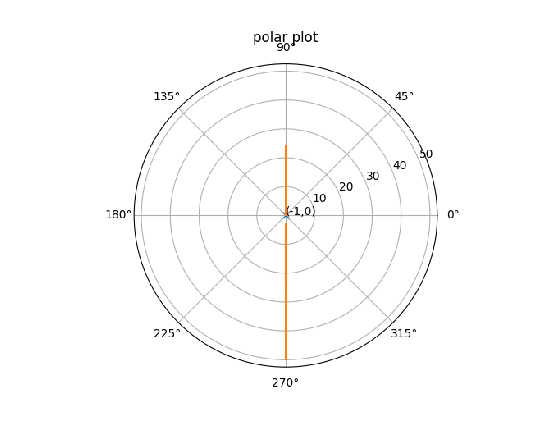
\includegraphics[width=\columnwidth]{./figs/ee18btech11023/ee18btech11023_1c.eps}
  \caption{}
  \label{fig:ee18btech11023}
\end{figure}
In Fig.   \ref{fig:ee18btech11023},  (–1,0) is exactly on the polar plot.  Hence, the system is marginally stable.


\end{enumerate}


\section{Nyquist Plot}
%%%%%%%%%%%%%%%%%%%%%%%%%%%%%%%%%%%%%%%%%%%%%%%%%%%%%%%%%%%%%%%%%%%%%%
%%                                                                  %%
%%  This is the header of a LaTeX2e file exported from Gnumeric.    %%
%%                                                                  %%
%%  This file can be compiled as it stands or included in another   %%
%%  LaTeX document. The table is based on the longtable package so  %%
%%  the longtable options (headers, footers...) can be set in the   %%
%%  preamble section below (see PRAMBLE).                           %%
%%                                                                  %%
%%  To include the file in another, the following two lines must be %%
%%  in the including file:                                          %%
%%        \def\inputGnumericTable{}                                 %%
%%  at the beginning of the file and:                               %%
%%        \input{name-of-this-file.tex}                             %%
%%  where the table is to be placed. Note also that the including   %%
%%  file must use the following packages for the table to be        %%
%%  rendered correctly:                                             %%
%%    \usepackage[latin1]{inputenc}                                 %%
%%    \usepackage{color}                                            %%
%%    \usepackage{array}                                            %%
%%    \usepackage{longtable}                                        %%
%%    \usepackage{calc}                                             %%
%%    \usepackage{multirow}                                         %%
%%    \usepackage{hhline}                                           %%
%%    \usepackage{ifthen}                                           %%
%%  optionally (for landscape tables embedded in another document): %%
%%    \usepackage{lscape}                                           %%
%%                                                                  %%
%%%%%%%%%%%%%%%%%%%%%%%%%%%%%%%%%%%%%%%%%%%%%%%%%%%%%%%%%%%%%%%%%%%%%%



%%  This section checks if we are begin input into another file or  %%
%%  the file will be compiled alone. First use a macro taken from   %%
%%  the TeXbook ex 7.7 (suggestion of Han-Wen Nienhuys).            %%
\def\ifundefined#1{\expandafter\ifx\csname#1\endcsname\relax}


%%  Check for the \def token for inputed files. If it is not        %%
%%  defined, the file will be processed as a standalone and the     %%
%%  preamble will be used.                                          %%
\ifundefined{inputGnumericTable}

%%  We must be able to close or not the document at the end.        %%
	\def\gnumericTableEnd{\end{document}}


%%%%%%%%%%%%%%%%%%%%%%%%%%%%%%%%%%%%%%%%%%%%%%%%%%%%%%%%%%%%%%%%%%%%%%
%%                                                                  %%
%%  This is the PREAMBLE. Change these values to get the right      %%
%%  paper size and other niceties.                                  %%
%%                                                                  %%
%%%%%%%%%%%%%%%%%%%%%%%%%%%%%%%%%%%%%%%%%%%%%%%%%%%%%%%%%%%%%%%%%%%%%%

	\documentclass[12pt%
			  %,landscape%
                    ]{report}
       \usepackage[latin1]{inputenc}
       \usepackage{fullpage}
       \usepackage{color}
       \usepackage{array}
       \usepackage{longtable}
       \usepackage{calc}
       \usepackage{multirow}
       \usepackage{hhline}
       \usepackage{ifthen}

	\begin{document}


%%  End of the preamble for the standalone. The next section is for %%
%%  documents which are included into other LaTeX2e files.          %%
\else

%%  We are not a stand alone document. For a regular table, we will %%
%%  have no preamble and only define the closing to mean nothing.   %%
    \def\gnumericTableEnd{}

%%  If we want landscape mode in an embedded document, comment out  %%
%%  the line above and uncomment the two below. The table will      %%
%%  begin on a new page and run in landscape mode.                  %%
%       \def\gnumericTableEnd{\end{landscape}}
%       \begin{landscape}


%%  End of the else clause for this file being \input.              %%
\fi

%%%%%%%%%%%%%%%%%%%%%%%%%%%%%%%%%%%%%%%%%%%%%%%%%%%%%%%%%%%%%%%%%%%%%%
%%                                                                  %%
%%  The rest is the gnumeric table, except for the closing          %%
%%  statement. Changes below will alter the table's appearance.     %%
%%                                                                  %%
%%%%%%%%%%%%%%%%%%%%%%%%%%%%%%%%%%%%%%%%%%%%%%%%%%%%%%%%%%%%%%%%%%%%%%

\providecommand{\gnumericmathit}[1]{#1} 
%%  Uncomment the next line if you would like your numbers to be in %%
%%  italics if they are italizised in the gnumeric table.           %%
%\renewcommand{\gnumericmathit}[1]{\mathit{#1}}
\providecommand{\gnumericPB}[1]%
{\let\gnumericTemp=\\#1\let\\=\gnumericTemp\hspace{0pt}}
 \ifundefined{gnumericTableWidthDefined}
        \newlength{\gnumericTableWidth}
        \newlength{\gnumericTableWidthComplete}
        \newlength{\gnumericMultiRowLength}
        \global\def\gnumericTableWidthDefined{}
 \fi
%% The following setting protects this code from babel shorthands.  %%
 \ifthenelse{\isundefined{\languageshorthands}}{}{\languageshorthands{english}}
%%  The default table format retains the relative column widths of  %%
%%  gnumeric. They can easily be changed to c, r or l. In that case %%
%%  you may want to comment out the next line and uncomment the one %%
%%  thereafter                                                      %%
\providecommand\gnumbox{\makebox[0pt]}
%%\providecommand\gnumbox[1][]{\makebox}

%% to adjust positions in multirow situations                       %%
\setlength{\bigstrutjot}{\jot}
\setlength{\extrarowheight}{\doublerulesep}

%%  The \setlongtables command keeps column widths the same across  %%
%%  pages. Simply comment out next line for varying column widths.  %%
\setlongtables

\setlength\gnumericTableWidth{%
	55pt+%
	35pt+%
	119pt+%
0pt}
\def\gumericNumCols{3}
\setlength\gnumericTableWidthComplete{\gnumericTableWidth+%
         \tabcolsep*\gumericNumCols*2+\arrayrulewidth*\gumericNumCols}
\ifthenelse{\lengthtest{\gnumericTableWidthComplete > \linewidth}}%
         {\def\gnumericScale{\ratio{\linewidth-%
                        \tabcolsep*\gumericNumCols*2-%
                        \arrayrulewidth*\gumericNumCols}%
{\gnumericTableWidth}}}%
{\def\gnumericScale{1}}

%%%%%%%%%%%%%%%%%%%%%%%%%%%%%%%%%%%%%%%%%%%%%%%%%%%%%%%%%%%%%%%%%%%%%%
%%                                                                  %%
%% The following are the widths of the various columns. We are      %%
%% defining them here because then they are easier to change.       %%
%% Depending on the cell formats we may use them more than once.    %%
%%                                                                  %%
%%%%%%%%%%%%%%%%%%%%%%%%%%%%%%%%%%%%%%%%%%%%%%%%%%%%%%%%%%%%%%%%%%%%%%

\ifthenelse{\isundefined{\gnumericColA}}{\newlength{\gnumericColA}}{}\settowidth{\gnumericColA}{\begin{tabular}{@{}p{55pt*\gnumericScale}@{}}x\end{tabular}}
\ifthenelse{\isundefined{\gnumericColB}}{\newlength{\gnumericColB}}{}\settowidth{\gnumericColB}{\begin{tabular}{@{}p{35pt*\gnumericScale}@{}}x\end{tabular}}
\ifthenelse{\isundefined{\gnumericColC}}{\newlength{\gnumericColC}}{}\settowidth{\gnumericColC}{\begin{tabular}{@{}p{119pt*\gnumericScale}@{}}x\end{tabular}}

\begin{tabular}[c]{%
	b{\gnumericColA}%
	b{\gnumericColB}%
	b{\gnumericColC}%
	}

%%%%%%%%%%%%%%%%%%%%%%%%%%%%%%%%%%%%%%%%%%%%%%%%%%%%%%%%%%%%%%%%%%%%%%
%%  The longtable options. (Caption, headers... see Goosens, p.124) %%
%	\caption{The Table Caption.}             \\	%
% \hline	% Across the top of the table.
%%  The rest of these options are table rows which are placed on    %%
%%  the first, last or every page. Use \multicolumn if you want.    %%

%%  Header for the first page.                                      %%
%	\multicolumn{3}{c}{The First Header} \\ \hline 
%	\multicolumn{1}{c}{colTag}	%Column 1
%	&\multicolumn{1}{c}{colTag}	%Column 2
%	&\multicolumn{1}{c}{colTag}	\\ \hline %Last column
%	\endfirsthead

%%  The running header definition.                                  %%
%	\hline
%	\multicolumn{3}{l}{\ldots\small\slshape continued} \\ \hline
%	\multicolumn{1}{c}{colTag}	%Column 1
%	&\multicolumn{1}{c}{colTag}	%Column 2
%	&\multicolumn{1}{c}{colTag}	\\ \hline %Last column
%	\endhead

%%  The running footer definition.                                  %%
%	\hline
%	\multicolumn{3}{r}{\small\slshape continued\ldots} \\
%	\endfoot

%%  The ending footer definition.                                   %%
%	\multicolumn{3}{c}{That's all folks} \\ \hline 
%	\endlastfoot
%%%%%%%%%%%%%%%%%%%%%%%%%%%%%%%%%%%%%%%%%%%%%%%%%%%%%%%%%%%%%%%%%%%%%%

\hhline{|-|-|-}
	 \multicolumn{1}{|p{\gnumericColA}|}%
	{\gnumericPB{\centering}\textbf{Variable}}
	&\multicolumn{1}{p{\gnumericColB}|}%
	{\gnumericPB{\centering}\textbf{Value}}
	&\multicolumn{1}{p{\gnumericColC}|}%
	{\gnumericPB{\raggedright}\textbf{Description}}
\\
\hhline{|---|}
	 \multicolumn{1}{|p{\gnumericColA}|}%
	{\gnumericPB{\centering}Z}
	&\multicolumn{1}{p{\gnumericColB}|}%
	{\gnumericPB{\centering}0}
	&\multicolumn{1}{p{\gnumericColC}|}%
	{\gnumericPB{\raggedright}Poles of $\frac{G(s)}{1+G(s)H(s)}$in right half of s plane}
\\
\hhline{|---|}
	 \multicolumn{1}{|p{\gnumericColA}|}%
	{\gnumericPB{\centering}P}
	&\multicolumn{1}{p{\gnumericColB}|}%
	{\gnumericPB{\centering}0}
	&\multicolumn{1}{p{\gnumericColC}|}%
	{\gnumericPB{\raggedright}Poles of $G(s)H(s)$ in right half of s plane}
\\
\hhline{|---|}
	 \multicolumn{1}{|p{\gnumericColA}|}%
	{\gnumericPB{\centering}N}
	&\multicolumn{1}{p{\gnumericColB}|}%
	{\gnumericPB{\centering}0}
	&\multicolumn{1}{p{\gnumericColC}|}%
	{\gnumericPB{\raggedright}No of clockwise encirclements of $G(s)H(s)$  about -1+j0 in the Nyquist plot}
\\
\hhline{|-|-|-|}
\end{tabular}

\ifthenelse{\isundefined{\languageshorthands}}{}{\languageshorthands{\languagename}}
\gnumericTableEnd



\section{Compensators}
\subsection{Phase Lead}
%\begin{enumerate}[label=\thesection.\arabic*.,ref=\thesection.\theenumi]
\numberwithin{equation}{enumi} 
\item 
The Transfer function of Phase Lead Compensator is given by \\

\begin{align}
D(s) = \frac{3(s+\frac{1}{3T})}{(s+\frac{1}{T})}
\end{align}

Find out the frequency (in rad/sec), at which $\angle D(j\omega)$ is maximum? \\
\label{prob:ee18btech11010_comp}
\solution
The basic requirement of the phase lead network is that all poles and zeros
of the transfer function of the network must lie on negative real axis
interlacing each other with a zero located as the nearest point to origin.

Substituting $s = j\omega$ in D(s), we get \\

\begin{align}
D(j\omega) = \frac{3(j\omega+\frac{1}{3T})}{(j\omega+\frac{1}{T})}
\end{align}

The phase of this transfer function $\phi(\omega)$ is given by,
\begin{align}
\phi(\omega) = \tan^{-1}(3\omega T)-\tan^{-1}(\omega T)
\end{align}

$\phi(\omega)$ has its maximum at $\omega_c$ Where $\phi '(\omega_c)=0$,

\begin{align}
\phi '(\omega_c) = 0 = \frac{3T}{1+(3\omega _c T)^2}-\frac{T}{1+(\omega _c T)^2}
\end{align}

After solving and Simplification , we have \\

\begin{align}
\omega _c ^2T^2 = \frac{1}{3}
\end{align}

\begin{align}
\omega _c = \sqrt{\frac{1}{3T^2}}
\end{align}

\item Verify your result through a plot.
\\
\solution 
The following plots the Phase value of the transfer function, 

\begin{figure}[htp]
	\centering
	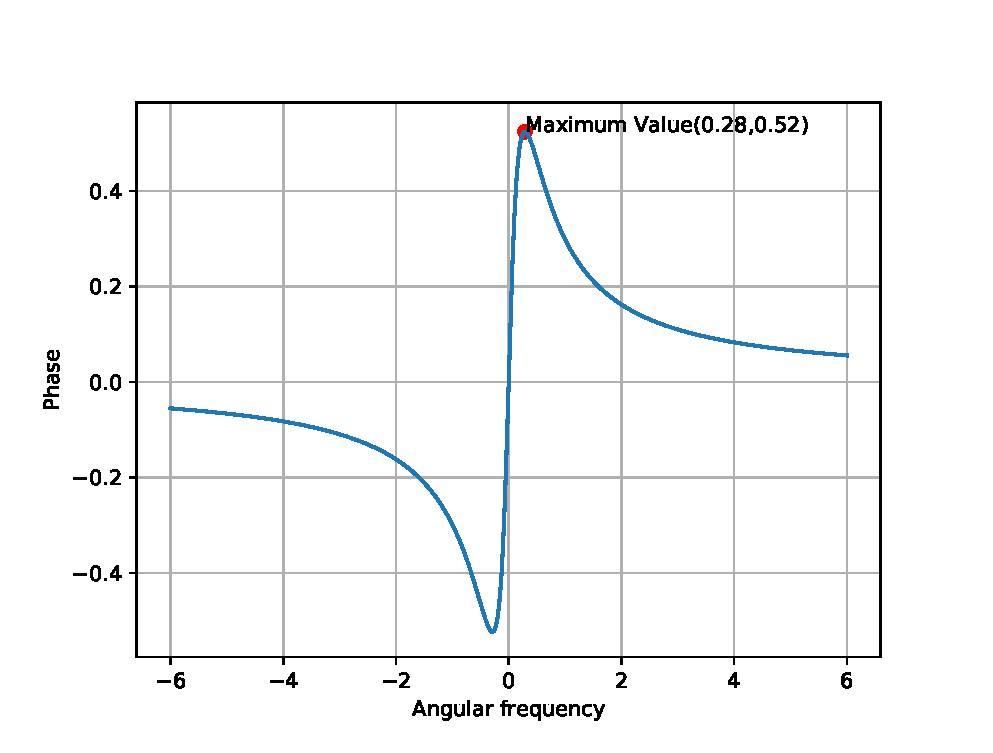
\includegraphics[width=\columnwidth]{./figs/ee18btech11010.eps}
	\caption{}
	\label{fig:ee18btech11010}
\end{figure}
 
\textbf{Applications:}\\ \\
\begin{enumerate}
  \item Phase lead Compensators can be used as High pass filters,Differentiators.
  \item They are used to reduce steady state errors. 
  \item Increases Phase Margin , relative stability.
\end{enumerate}
\item What is purpose of of a Phase Lead Compensator?
\item Through an example, show how the compensator in Problem \ref{prob:ee18btech11010_comp} can be used in a control system.



\end{enumerate}



%%%%%%%%%%%%%%%%%%%%%%%%%%%%%%%%%%%%%%%%%%%%%%%%%%%%%%%%%%%%%%%%%%%%%%
%%                                                                  %%
%%  This is the header of a LaTeX2e file exported from Gnumeric.    %%
%%                                                                  %%
%%  This file can be compiled as it stands or included in another   %%
%%  LaTeX document. The table is based on the longtable package so  %%
%%  the longtable options (headers, footers...) can be set in the   %%
%%  preamble section below (see PRAMBLE).                           %%
%%                                                                  %%
%%  To include the file in another, the following two lines must be %%
%%  in the including file:                                          %%
%%        \def\inputGnumericTable{}                                 %%
%%  at the beginning of the file and:                               %%
%%        \input{name-of-this-file.tex}                             %%
%%  where the table is to be placed. Note also that the including   %%
%%  file must use the following packages for the table to be        %%
%%  rendered correctly:                                             %%
%%    \usepackage[latin1]{inputenc}                                 %%
%%    \usepackage{color}                                            %%
%%    \usepackage{array}                                            %%
%%    \usepackage{longtable}                                        %%
%%    \usepackage{calc}                                             %%
%%    \usepackage{multirow}                                         %%
%%    \usepackage{hhline}                                           %%
%%    \usepackage{ifthen}                                           %%
%%  optionally (for landscape tables embedded in another document): %%
%%    \usepackage{lscape}                                           %%
%%                                                                  %%
%%%%%%%%%%%%%%%%%%%%%%%%%%%%%%%%%%%%%%%%%%%%%%%%%%%%%%%%%%%%%%%%%%%%%%



%%  This section checks if we are begin input into another file or  %%
%%  the file will be compiled alone. First use a macro taken from   %%
%%  the TeXbook ex 7.7 (suggestion of Han-Wen Nienhuys).            %%
\def\ifundefined#1{\expandafter\ifx\csname#1\endcsname\relax}


%%  Check for the \def token for inputed files. If it is not        %%
%%  defined, the file will be processed as a standalone and the     %%
%%  preamble will be used.                                          %%
\ifundefined{inputGnumericTable}

%%  We must be able to close or not the document at the end.        %%
	\def\gnumericTableEnd{\end{document}}


%%%%%%%%%%%%%%%%%%%%%%%%%%%%%%%%%%%%%%%%%%%%%%%%%%%%%%%%%%%%%%%%%%%%%%
%%                                                                  %%
%%  This is the PREAMBLE. Change these values to get the right      %%
%%  paper size and other niceties.                                  %%
%%                                                                  %%
%%%%%%%%%%%%%%%%%%%%%%%%%%%%%%%%%%%%%%%%%%%%%%%%%%%%%%%%%%%%%%%%%%%%%%

	\documentclass[12pt%
			  %,landscape%
                    ]{report}
       \usepackage[latin1]{inputenc}
       \usepackage{fullpage}
       \usepackage{color}
       \usepackage{array}
       \usepackage{longtable}
       \usepackage{calc}
       \usepackage{multirow}
       \usepackage{hhline}
       \usepackage{ifthen}

	\begin{document}


%%  End of the preamble for the standalone. The next section is for %%
%%  documents which are included into other LaTeX2e files.          %%
\else

%%  We are not a stand alone document. For a regular table, we will %%
%%  have no preamble and only define the closing to mean nothing.   %%
    \def\gnumericTableEnd{}

%%  If we want landscape mode in an embedded document, comment out  %%
%%  the line above and uncomment the two below. The table will      %%
%%  begin on a new page and run in landscape mode.                  %%
%       \def\gnumericTableEnd{\end{landscape}}
%       \begin{landscape}


%%  End of the else clause for this file being \input.              %%
\fi

%%%%%%%%%%%%%%%%%%%%%%%%%%%%%%%%%%%%%%%%%%%%%%%%%%%%%%%%%%%%%%%%%%%%%%
%%                                                                  %%
%%  The rest is the gnumeric table, except for the closing          %%
%%  statement. Changes below will alter the table's appearance.     %%
%%                                                                  %%
%%%%%%%%%%%%%%%%%%%%%%%%%%%%%%%%%%%%%%%%%%%%%%%%%%%%%%%%%%%%%%%%%%%%%%

\providecommand{\gnumericmathit}[1]{#1} 
%%  Uncomment the next line if you would like your numbers to be in %%
%%  italics if they are italizised in the gnumeric table.           %%
%\renewcommand{\gnumericmathit}[1]{\mathit{#1}}
\providecommand{\gnumericPB}[1]%
{\let\gnumericTemp=\\#1\let\\=\gnumericTemp\hspace{0pt}}
 \ifundefined{gnumericTableWidthDefined}
        \newlength{\gnumericTableWidth}
        \newlength{\gnumericTableWidthComplete}
        \newlength{\gnumericMultiRowLength}
        \global\def\gnumericTableWidthDefined{}
 \fi
%% The following setting protects this code from babel shorthands.  %%
 \ifthenelse{\isundefined{\languageshorthands}}{}{\languageshorthands{english}}
%%  The default table format retains the relative column widths of  %%
%%  gnumeric. They can easily be changed to c, r or l. In that case %%
%%  you may want to comment out the next line and uncomment the one %%
%%  thereafter                                                      %%
\providecommand\gnumbox{\makebox[0pt]}
%%\providecommand\gnumbox[1][]{\makebox}

%% to adjust positions in multirow situations                       %%
\setlength{\bigstrutjot}{\jot}
\setlength{\extrarowheight}{\doublerulesep}

%%  The \setlongtables command keeps column widths the same across  %%
%%  pages. Simply comment out next line for varying column widths.  %%
\setlongtables

\setlength\gnumericTableWidth{%
	53pt+%
	93pt+%
0pt}
\def\gumericNumCols{2}
\setlength\gnumericTableWidthComplete{\gnumericTableWidth+%
         \tabcolsep*\gumericNumCols*2+\arrayrulewidth*\gumericNumCols}
\ifthenelse{\lengthtest{\gnumericTableWidthComplete > \linewidth}}%
         {\def\gnumericScale{\ratio{\linewidth-%
                        \tabcolsep*\gumericNumCols*2-%
                        \arrayrulewidth*\gumericNumCols}%
{\gnumericTableWidth}}}%
{\def\gnumericScale{1}}

%%%%%%%%%%%%%%%%%%%%%%%%%%%%%%%%%%%%%%%%%%%%%%%%%%%%%%%%%%%%%%%%%%%%%%
%%                                                                  %%
%% The following are the widths of the various columns. We are      %%
%% defining them here because then they are easier to change.       %%
%% Depending on the cell formats we may use them more than once.    %%
%%                                                                  %%
%%%%%%%%%%%%%%%%%%%%%%%%%%%%%%%%%%%%%%%%%%%%%%%%%%%%%%%%%%%%%%%%%%%%%%

\ifthenelse{\isundefined{\gnumericColA}}{\newlength{\gnumericColA}}{}\settowidth{\gnumericColA}{\begin{tabular}{@{}p{53pt*\gnumericScale}@{}}x\end{tabular}}
\ifthenelse{\isundefined{\gnumericColB}}{\newlength{\gnumericColB}}{}\settowidth{\gnumericColB}{\begin{tabular}{@{}p{93pt*\gnumericScale}@{}}x\end{tabular}}

\begin{tabular}[c]{%
	b{\gnumericColA}%
	b{\gnumericColB}%
	}

%%%%%%%%%%%%%%%%%%%%%%%%%%%%%%%%%%%%%%%%%%%%%%%%%%%%%%%%%%%%%%%%%%%%%%
%%  The longtable options. (Caption, headers... see Goosens, p.124) %%
%	\caption{The Table Caption.}             \\	%
% \hline	% Across the top of the table.
%%  The rest of these options are table rows which are placed on    %%
%%  the first, last or every page. Use \multicolumn if you want.    %%

%%  Header for the first page.                                      %%
%	\multicolumn{2}{c}{The First Header} \\ \hline 
%	\multicolumn{1}{c}{colTag}	%Column 1
%	&\multicolumn{1}{c}{colTag}	\\ \hline %Last column
%	\endfirsthead

%%  The running header definition.                                  %%
%	\hline
%	\multicolumn{2}{l}{\ldots\small\slshape continued} \\ \hline
%	\multicolumn{1}{c}{colTag}	%Column 1
%	&\multicolumn{1}{c}{colTag}	\\ \hline %Last column
%	\endhead

%%  The running footer definition.                                  %%
%	\hline
%	\multicolumn{2}{r}{\small\slshape continued\ldots} \\
%	\endfoot

%%  The ending footer definition.                                   %%
%	\multicolumn{2}{c}{That's all folks} \\ \hline 
%	\endlastfoot
%%%%%%%%%%%%%%%%%%%%%%%%%%%%%%%%%%%%%%%%%%%%%%%%%%%%%%%%%%%%%%%%%%%%%%

\hhline{|-|-}
	 \multicolumn{1}{|p{\gnumericColA}|}%
	{\gnumericPB{\centering}\gnumbox{\textbf{Controller}}}
	&\multicolumn{1}{p{\gnumericColB}|}%
	{\gnumericPB{\centering}\gnumbox{\textbf{Gain}}}
\\
\hhline{|--|}
	 \multicolumn{1}{|p{\gnumericColA}|}%
	{\gnumericPB{\centering}\gnumbox{PID}}
	&\multicolumn{1}{p{\gnumericColB}|}%
	{$    K_{p}\brak{1 + T_{d}s + \frac{1}{T_{i}s}}$}
\\
\hhline{|--|}
	 \multicolumn{1}{|p{\gnumericColA}|}%
	{\gnumericPB{\centering}\gnumbox{PD}}
	&\multicolumn{1}{p{\gnumericColB}|}%
	{$    K_{p}(1 + T_{d}s)$}
\\
\hhline{|--|}
	 \multicolumn{1}{|p{\gnumericColA}|}%
	{\gnumericPB{\centering}\gnumbox{PI}}
	&\multicolumn{1}{p{\gnumericColB}|}%
	{$    K_{p}\brak{1 +  \frac{1}{T_{i}s}}$}
\\
\hhline{|-|-|}
\end{tabular}

\ifthenelse{\isundefined{\languageshorthands}}{}{\languageshorthands{\languagename}}
\gnumericTableEnd

\section{Oscillator}
\begin{enumerate}[label=\thesection.\arabic*.,ref=\thesection.\theenumi]
\numberwithin{equation}{enumi}

\item Fig. \label{fig:ee18btech11019_hart} shows a Hartley oscillator.

\begin{figure}[ht]
    \begin{center}
	    \resizebox{\columnwidth}{!}{\begin{circuitikz} [scale=2]  \draw 
(0,0) node[op amp] (opamp) [scale=2] {}
(opamp.-) -- (-3,0.5) to [R=$R_1$] (-5,0.5) -- (-6,0.5) -- (-6,-2) to [L=$L_2$] (-4,-2)
-- (-1,-2) to[L=$L_1$] (1,-2) -- (1,0) {};
\node[draw,box] (A) at (1.5,-0.7) {$V_{out}$};
\draw (-6,-2) -- (-6,-3)  to [C=$C$] (1,-3) -- (1,-2) 

(opamp.-) to[short,*-] ++(0,1) coordinate (leftC)
to[R=$R_2$] (leftC -| opamp.out)
to[short,-*] (opamp.out) to [short,-o] (1.5,0) to (1.5,-0.5) {}
(opamp.+) -- (-3,-0.5) to [R=$R_3$] (-5,-0.5) node[ground] [scale=2] {};
\draw (-2,-0.5) -- (-2,-2);


\end{circuitikz}
}
	\end{center}
\caption{Hartley oscillator}
\label{fig:ee18btech11019_hart}
\end{figure}
Draw the equivalent block diagram.
\solution  The block diagram is available in Fig. \label{fig:ee18btech11019_hart_block}
\begin{figure}[!ht]
    \begin{center}
		
		\resizebox{\columnwidth}{!}{\tikzset{
        amp/.style = {regular polygon, regular polygon sides=3,
              draw, fill=white, text width=1em,
              inner sep=1mm, outer sep=0mm,
              shape border rotate=-90},
        block/.style = {draw, rectangle,
            minimum height=1cm,
            minimum width=2cm},
        input/.style = {coordinate,node distance=1cm},
        output/.style = {coordinate,node distance=4cm},
        arrow/.style={draw, -latex,node distance=2cm},
        pinstyle/.style = {pin edge={latex-, black,node distance=2cm}},
        sum/.style = {draw, circle, node distance=1cm},
}

\begin{tikzpicture}[node distance=2.5cm,auto,>=latex']
  \node [input, name=input] {};
  \node [sum, right of=input] (sum) {};
  \node [amp, right of = sum] (block1) {$A$};
  \node [output, right of= block1] (output) {};
  \node [block, below of = block1] (block2) {$B$};
  \draw [->] (input) -- node {$V_{in}$} (sum);
  \draw [->] (sum) -- node {$V_{in} + BV_{out}$} (block1);
  \draw [->] (block1) -- node [name =y] {$V_{out}$} (output);
  \draw [->] (y) |- node [above,pos=0.79] {$V_{out}$} (block2) ;
  \draw [->] (block2) -| node  {$BV_{out}$} (sum) ;
\end{tikzpicture}
} %block diagram
	\end{center}
\caption{block diagram for oscillator}
\label{fig:ee18btech11019_hart_block}
\end{figure}
%
\item Find the gain of the oscillator. 
\\
\solution The control system in Fig. \ref{fig:ee18btech11019_hart_block} has positive feedback.  Hence, the gain is 

\begin{align}
    G = \frac{G(s)}{1-G(s)H(s)}
\label{eq:ee18btech11019_gain}
\end{align}
%
\item Find $G(s)$ and $H(s)$.
\\
\solution From figure \ref{fig:ee18btech11019_hart_block}
Oscillators gain can be given as follows:\\
\begin{align}
    A(V_{in} + BV_{out}) =V_{out}\\
    A(V_{in} = (1-AB)V_{out}\\
    \frac{V_{out}}{V_{in}} = \frac{A}{1 - AB}
\end{align}
%
resulting in \eqref{eq:ee18btech11019_gain}.\\



\item State the condition for sustained oscillations. Justify.

\solution Condition for sustained oscillation is given by\\
\begin{align}
    AB = 1
\end{align}
Along with, total phase gain o the circuit should be 0 or 2$\pi$\\
\textbf{Justification:} as, when $ AB =1 $, gain becomes infinity, and theoretically we can get output, without actually providing input\\
Total phase gain should be so, as we want our signal to be in phase after every loop traversal.\\


\item Find $A$ and $B$.

\solution Consider the below circuit fig \ref{fig:ee18btech11019_block2},its basic form of a LC oscillator.\\
%\begin{figure}[!ht]
%    \begin{center}
%		\resizebox{\columnwidth}{!}{\begin{circuitikz} 
(0,0) node[op amp] (opamp) [scale=2] {}
\draw
(0,0) -- (4,0) node[label = $V_{out}$]
  to [european resistor = $Z_2$]  (4,-4)   -- (0,-4)node[ground] {} to[european resistor = $Z_1$] (0,-2) 
  to[european resistor = $Z_3$] (0,0);
  \draw 
    (-2,0) node[op amp] (opamp) {} 
    (0,0) -- (opamp.out)
    (opamp.+)--(-4,-0.5)--(-4,-1)node[ground] {}
  (0,-2)--(-6,-2)--(-6,0.5) -- (opamp.-);
  

\end{circuitikz} 
}
%		
%	\end{center}
%\caption{block diagram for oscillator}
%\label{fig:ee18btech11019_block2}
%\end{figure}
The above figure \ref{fig:ee18btech11019_block2} can also be drawn as fig. \ref{fig:ee18btech11019_block3},when feedback is considered as load :\\
%\begin{figure}[!ht]
%    \begin{center}
%		\resizebox{\columnwidth}{!}{\begin{circuitikz} 

\draw
(0,0) -- (4,0) node[label = $V_{out}$]
  to [european resistor = $Z_2$]  (4,-4)   -- (0,-4)node[ground] {} to[european resistor = $Z_1$] (0,-2) 
  to[european resistor = $Z_3$] (0,0) to[american resistor,label=$R_o$] (-4,0) to[american voltage source ,label= -$A_vV_{in}$](-4,-1) node[ground] {}
  (0,-2)--(-6,-2)--(-6,0) node[label = $V_f$];
  

\end{circuitikz} 
}
%		
%	\end{center}
%\caption{block diagram for oscillator}
%\label{fig:ee18btech11019_block3}
%\end{figure}
We know that feedback gain is B, i.e, $\frac{V_0}{V_f} = B$\\
Applying voltage divider rule we get\\
From figure \ref{fig:ee18btech11019_block2}
\begin{align}
    B = \frac{Z_1}{Z_1 + Z_3}
\end{align}
From fig. \eqref{fig:ee18btech11019_block3}
\begin{align}
    A = \frac{V_o}{V_{in}} = \frac{A_vZ_L}{R_o + Z_L}\\
\end{align}    
    where,\\
    $A_v$ is the amplification factor of the opamp\\
    $v_{in}$ is the internal voltage in amplifier\\
    $Z_L$ is equivalent load across output
         
\begin{align}    
    Z_L = \frac{(Z_1 + Z_3)Z_2}{Z_1+Z_2+Z_3}
\end{align}


\item Find the frequency of oscillation using the condition that $AB = 1$.

\solution For any LC oscillator, 
Now,we know that $AB = 1$ for sustained oscillations, putting the the above terms in the equation\\
on solving,\\
\begin{align}    
    AB = \frac{Z_1Z_2A}{(Z_1+Z_2+Z_3)R_o+ Z_2(Z_1+Z_3)}
\end{align}    
\textbf{Hartley oscillator}:\\
The Hartley oscillator is one of the classical LC feedback circuits,i.e feedback is made of LC components.Below here 
\begin{align}
    Z_1 = SL_1 (inductor)\\
    Z_2 = SL_2 (inductor)\\
    Z_3 = \frac{1}{SC} (capacitor)
\end{align}

putting that in and equating $AB=1$ we get,

\begin{align}
1 = \frac{S^{2}L_1L_2A}{(SL_1+SL_2+\frac{1}{SC})R_o+ SL_2(SL_1+\frac{1}{SC})}\\
S^{2}L_1L_2A = (SL_1+SL_2+\frac{1}{SC})R_o+ SL_2(SL_1+\frac{1}{SC})
\end{align}

As we need, to find frequency, put S =jw
\begin{align}
    \omega^{2}L_1L_2A = j(\omega L_1 + \omega L_2 -\frac{1}{\omega C})R_o -\omega L_2(\omega L_1 + \frac{1}{\omega C})
\end{align}
To satisfy the above equation, equating imaginary term to Zero.
\begin{align}    
    \omega L_1 + \omega L_2  = \frac{1}{\omega C}\\
    \omega = \frac{1}{\sqrt{(L_1+L_2)(C)}}\\
    f = \frac{1}{2\pi \sqrt{(L_1+L_2)(C)}}
\end{align}
\begin{align}
    B = \frac{Z_1}{Z_1 + Z_3} = \frac{Z_1}{Z_2}\\
      = \frac{L_1}{L_2}
    \label{eq:ee18btech11019_B_gain}  
\end{align}
\begin{align}
    A =  \frac{L_2}{L_1} 
\label{eq:ee18btech11019_Amp_gain}
\end{align}
 
\item For Hartley oscillator frequency generated can be given as 
\begin{align}
    f = \frac{1}{2\pi\sqrt{(L_1 + L_2)C}}
    \label{eq:ee18btech11019_frequency}
\end{align}
Fig. \ref{fig:ee18btech11019_hart} shows a
Hartley oscillator built using opamp.\\

We can easily compare between \ref{fig:ee18btech11019_hart_block} and \ref{fig:ee18btech11019_hart}\\
We know that for an opamp A is given by:
\begin{align}
    A = \frac{R_2}{R_1}
\end{align}
Here,
\begin{align}
    A(S) = \frac{R_2}{R_1} = \frac{L_2}{L_1}
\end{align}
referring to \ref{eq:ee18btech11019_Amp_gain}\\
And,
\begin{align}
    B(s) = \frac{V_o}{V_f} = \frac{L_1}{L_2}
\end{align}
referring to \ref{eq:ee18btech11019_B_gain}\\
\newline
\item \textbf{Simulation:}\\
Taking the following values,and applying in \ref{eq:ee18btech11019_frequency} \\



\begin{tabular}{|c|c|}
\hline
Component & Value  \\
\hline
$R_1$         & 10K$\Omega$   \\
\hline
$R_2$         & 100K$\Omega$   \\
\hline
$R_3$         & $\sim$  \\
\hline
$L_1$         & $1 \mu H$     \\
\hline
$L_2$         & $1 \mu H$   \\
\hline
C         & 120 pF \\
\hline
\end{tabular}


We get f = 103 MHz\\
Feedback factor for Hartley given by:
\begin{align}
B =\frac{L_1}{L_2}= 1
\end{align}
W.K.T, $AB = 1$\\
$\therefore$ Minimum amplification Gain,A = 1\\
\end{enumerate}

\section{Gain Margin}
\begin{enumerate}[label=\thesubsection.\arabic*.,ref=\thesubsection.\theenumi]
\numberwithin{equation}{enumi} 
\item The open loop transfer function of a feedback control system is  
\begin{align}
G(s) = \frac{1}{s(1+2s)(1+s)} 
\label{ee18btech11016_gs}
\end{align}
%
Find the magnitude and phase of $\abs{G\brak{\j\omega}}$.
\\
\solution
\begin{align}
G\brak{\j\omega} &= \frac{1}{\j\omega(1+2\j\omega)(1+\j\omega)} 
\\
 &= \frac{1}{\j\omega(1+3\j\omega-2\omega^2)}
\\
&=\frac{1}{\j\omega-3\omega^2-2\j\omega^3}
\\
 &= \frac{1}{-3\omega^2+\j\omega(1-2\omega^2)} 
\\
\implies \angle G\brak{\j\omega}&=- tan^{-1}\brak{\frac{\omega(1-2\omega^2)}{-3\omega^2}}
\label{ee18btech11016_gs_ang}
\end{align}
%
\item The frequency at which the phase of open-loop transfer function reaches -180$\degree$ or +180$\degree$ depending upon the range of tan inverse function) is defined to be the phase crossover frequency.  Find the phase crossover frequency for  \eqref{ee18btech11016_gs}.
\solution From \eqref{ee18btech11016_gs_ang}, at $\omega=\omega_{pc}$ 
\begin{align}
\omega(1-2\omega^2) = 0 
\\
\implies \omega_{pc} = \frac{1}{\sqrt{2}} 
\end{align}
\item The gain Margin is given by,
\begin{align}
GM = -20log_{10}\abs{G\brak{\j\omega_{pc}}} = 20log_{10}k_{g}
\end{align}
where 
\begin{align}
k_{g}=\frac{1}{\abs{G\brak{\j\omega_{pc}}}} 
\end{align}
%
Find the GM for \eqref{ee18btech11016_gs_ang}.
\\
\solution 
\begin{align}
\abs{G\brak{\j\omega_{pc}}} &= \frac{1}{\brak{\frac{3}{2}}}
\implies k_{g}&=\frac{1}{\abs{G\brak{\j\omega_{pc}}}} = \frac{3}{2}
3.5dB
\end{align}
The greater the Gain Margin (GM), the greater the stability of the system. The gain margin refers to the amount of gain, which can be increased or decreased without making the system unstable. It is usually expressed as a magnitude in dB.
\item Obtain the GM from the Bode plot.
\\
\solution The following code 
\begin{lstlisting}
codes/ee18btech11016.py
\end{lstlisting}
%
plots the amplitude and phase of \eqref{ee18btech11016_gs} in Fig. \ref{fig:ee18btech11016}.
%
\begin{figure}[htp]
	\centering
	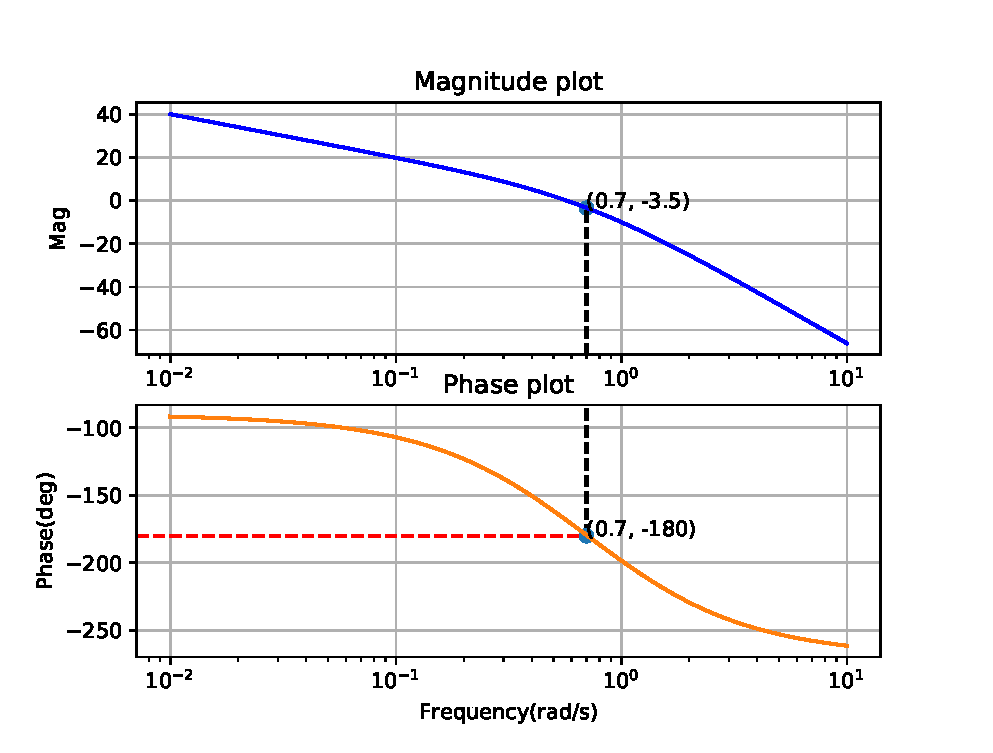
\includegraphics[width=\columnwidth]{./figs/ee18btech11016/ee18btech11016.eps}
	\caption{}
	\label{fig:ee18btech11016}
\end{figure}
From Fig. \ref{fig:ee18btech11016},
\begin{align}
20\log_{10}\abs{G\brak{\j\omega_{pc}}} &= -3.5dB,  \quad \omega_{pc} = -180\degree
\\
\implies  GM &= +3.5dB. 
\end{align}
\item A positive GM indicates closed loop stability with unity feedback.  Verify this for \eqref{ee18btech11016_gs}.
\\
\solution 
The characteristic equation is 
\begin{align}
1+G(s)=0 
\implies 2s^3 + 3s^2 + s + 1 = 0 
\end{align}
Constructing the routh array
\begin{align}
\mydet{s^3\\s^2\\s}
\mydet{2 & 1 & 0 \\ 3 & 1 & 0 \\ (1/3) & 0 & 0}
\\
\mydet{s^3\\s^2\\s\\s^0}
\mydet{2 & 1 & 0 \\ 3 & 1 & 0 \\ (1/3) & 0 & 0 \\ 1 & 0 & 0}
\end{align}\\
%
There are no sign changes in the first column of the routh array. 
$\therefore$ the system is stable.

\item Instead of unity feedback, consider a system with 
%
\begin{align}
H(s)=\frac{1}{s+1}
\end{align}
%
Find the magnitude and phase of $\abs{G\brak{\j\omega}H\brak{\j\omega}}$
\\
\solution 
%
\begin{align}
\because G(s)H(s) & =\frac{1}{s(1+2s)(s+1)^{2}},
\\
G\brak{\j\omega}H\brak{\j\omega} &= \frac{1}{(2\omega^4-4\omega^2) +j(\omega-5\omega^3)}
\\
\implies \angle G\brak{\j\omega}H\brak{\j\omega} &= -tan^{-1}(\frac{\omega-5\omega^3}{2\omega^4-4\omega^2})
\end{align}

\item Compute the open loop gain margin for this system.
\\
\solution 
For $\omega$=$\omega_{pc}$ 

\begin{align}
\text{Im}\cbrak{G\brak{\j\omega}H\brak{\j\omega}}&=0. 
\\
\implies\omega(1-5\omega^2)=0
\\
\implies\omega_{pc} = \frac{1}{\sqrt{5}}
\end{align}
Hence, 
\begin{align}
GM = -20log_{10}|G\brak{\j\omega_{pc}}H\brak{\j\omega_{pc}}| = 20log_{10}k_{g}
\end{align}
where 
\begin{align}
k_{g}&=\frac{1}{|G\brak{\j\omega_{pc}}H\brak{\j\omega_{pc}}|}
\\
&= \frac{ 18}{25} = 2.853dB.
\end{align}
%
Hence $GM < 0$ and the system is unstable.
%
\item Obtain the GM from the Bode plot.
\\
\solution The following code 
\begin{lstlisting}
codes/ee18btech11016_2.py
\end{lstlisting}
%
plots the amplitude and phase of \eqref{ee18btech11016_gs} in Fig. \ref{fig:ee18btech11016_2}.
%
\begin{figure}[htp]
	\centering
	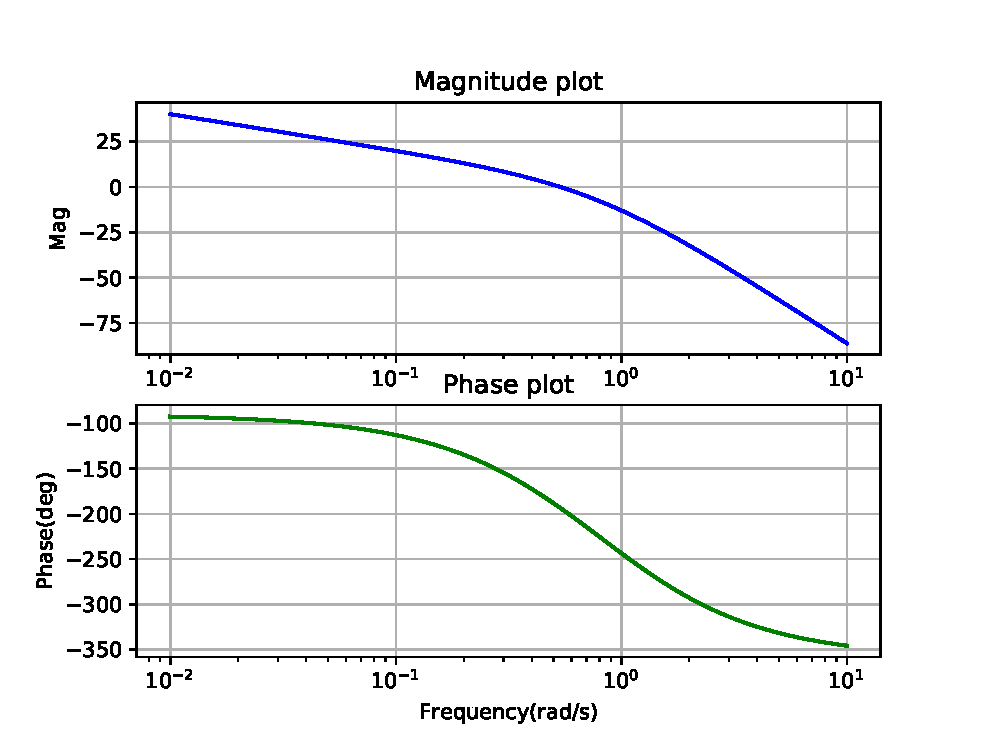
\includegraphics[width=\columnwidth]{./figs/ee18btech11016/ee18btech11016_2.eps}
	\caption{}
	\label{fig:ee18btech11016_2}
\end{figure}
\item Show that the closed loop transfer function 
\begin{align}
T(s) = \frac{1}{1 + (s(1+2s)(1+s)^2)}
\end{align}
%
is unstable using the Routh Hurwitz criterion.
\\
\solution 
The characteristics equation is 
\begin{align}
2s^4 + 5s^3 + 4s^3 + s + 1 = 0 
\end{align}
Constructing routh array for the above,
\begin{align}
\mydet{s^4\\s^3\\s^2}
\mydet{2 & 4 & 1 \\ 5 & 1 & 0 \\ (18/5) & 1 & 0}
\\
\mydet{s^4\\s^3\\s^2\\s}
\mydet{2 & 1 & 0 \\ 3 & 1 & 0 \\ (18/5) & 1 & 0 \\ (-7/18) & 0 & 0}
\\
\mydet{s^4\\s^3\\s^2\\s\\s^0}
\mydet{2 & 1 & 0 \\ 3 & 1 & 0 \\ (18/5) & 1 & 0 \\ (-7/18) & 0 & 0 \\ 1 & 0 & 0}
\end{align}
%
There are 2 sign changes in the first column of the routh array. So, 2 poles lie on right half of s-plane.
Therefore,the system is unstable.
%
\end{enumerate}



\section{Phase Margin}
\begin{enumerate}[label=\thesection.\arabic*.,ref=\thesection.\theenumi]
\numberwithin{equation}{enumi}

\item The open loop transfer function of a system is 
\begin{align}
G(s) = \frac{2}{(s+1)(s+2)}
\label{eq:ee18btech11017_system}
\end{align}
Find its magnitude and phase response.
\\
\solution Substituting $s = \j\omega$ in \eqref{eq:ee18btech11017_system},

\begin{align}
G\brak{\j\omega}&=\frac{1}{\brak{j\omega+1}\brak{j\omega+2}} 
\\
\implies 
\abs{G\brak{\j\omega}}&=\frac{2}{\brak{\sqrt{\omega^2+1}}\brak{\sqrt{\omega^2+4}}}
\label{eq:ee18btech11017_gain}
\\
\angle G\brak{\j\omega}&=- \tan^{-1}(\omega) - \tan^{-1}\brak{\frac{\omega}{2}} 
\label{eq:ee18btech11017_phase}
\end{align}

\item Find $\omega$ for which the gain of \eqref{eq:ee18btech11017_system} first becomes 1.
\\
\solution From \eqref{eq:ee18btech11017_gain}

\begin{align}
\abs{G\brak{\j\omega}}&=1
\\
\implies \frac{2}{\brak{\sqrt{\omega^2+1}}\brak{\sqrt{\omega^2+4}}}&=1
\\
\implies \omega_{gc}&=0
\end{align}
which is the desired frequency.

\item Find $\angle G(\j\omega_{gc}) + 180\degree$.  This is known as the {\em phase margin}(PM)
\\
\solution From \eqref{eq:ee18btech11017_phase},
%
\begin{align}
\angle G\brak{\j\omega} = 0\degree
\implies PM=180\degree
\label{eq:ee18btech11017_pm}
\end{align}
%
\item Verify your result by plotting the gain and phase plots of $G(\j\omega)$.
\\
\solution The following code plots Fig. \ref{fig:ee18btech11017}

\begin{lstlisting}
codes/ee18btech11017.py
\end{lstlisting}
%
The Phase plot is as shown,
\begin{figure}[!h]
  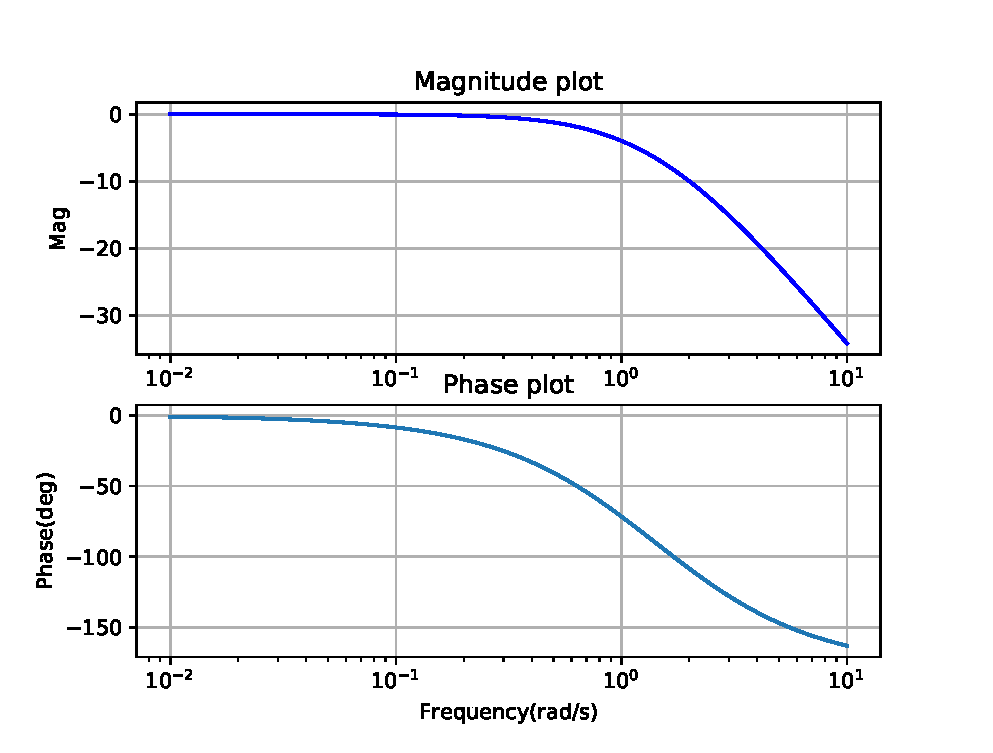
\includegraphics[width=\columnwidth]{./figs/ee18btech11017/ee18btech11017.eps}
  \caption{}
  \label{fig:ee18btech11017}
\end{figure}

\item A positive phase margin for the open loop system indicates a stable closed loop system.  \eqref{eq:ee18btech11017_pm} indicates that $G(s)$ with unity feedback is stable.  Show that the roots of $1+G(s)$ lie in the left half plane proving closed loop stability.
\\
\solution  Let the closed loop transfer function
\begin{align}
T(s)=\frac{G(s)}{1+G(s)}
\end{align}
Then
\begin{align}
1+G(s)&=0 
\\
\implies s^{2}+3s+4&=0 
\\
\text{or } s&=-1.5+1.3j,-1.5-1.3j
\end{align}
Since the roots are in the left half plane, the system is stable.
%

\item Instead of unity feedback, consider a system with 
%
\begin{align}
H(s)=\frac{50}{s+1}
\end{align}
%
Compute the open loop phase margin for this system.
\\
\solution 
%
\begin{align}
\because G(s)H(s)=\frac{100}{(s+1)^{2}(s+2)},
\label{eq:ee18btech11017_gh}
\end{align}
%
the  magnitude and phase are
\begin{align}
\label{eq:ee18btech11017_gh_mag}
\abs{G\brak{\j\omega}H\brak{\j\omega}}&=\frac{10^{2}}{ \sqrt{(\omega^{2}+1)^{2}}
\sqrt{\omega^{2}+4}} \\
\angle G\brak{\j\omega}H\brak{\j\omega}&=-\tan^{-1}\frac{\omega}{2}-2\tan^{-1}(\omega) 
\label{eq:ee18btech11017_gh_ang}
\end{align}
%
The gain crossover frequency is given by 
\begin{align}
\frac{10^{2}}{\sqrt{\omega_{gc}^{2}+4} \sqrt{(\omega_{gc}^{2}+10^{2})^{2}}}&=1 \\
\\
\omega_{gc}^{6}+6\omega_{gc}^{4}+9\omega_{gc}^{2}-9996&=0 
\\
\implies \omega_{gc} &= 4.42  
\label{eq:ee18btech11017_gh_wgc}
\end{align}
%
From \eqref{eq:ee18btech11017_gh_ang} and \eqref{eq:ee18btech11017_gh_wgc},
the phase margin is
\begin{align}
PM &=180\degree-2\tan^{-1}(\omega_{gc})-\tan^{-1}\brak{\frac{\omega_{gc}}{2}} \\
\implies  P.M &=-40.15\degree
\label{eq:ee18btech11017_gh_pm}
\end{align}
\item Verify your result through the magnitude and phase plot.
\\
\solution The following code plots Fig. \ref{fig:ee18btech11017_2}
\begin{lstlisting}
codes/ee18btech11017_2.py
\end{lstlisting}
%\begin{figure}[!h]
%  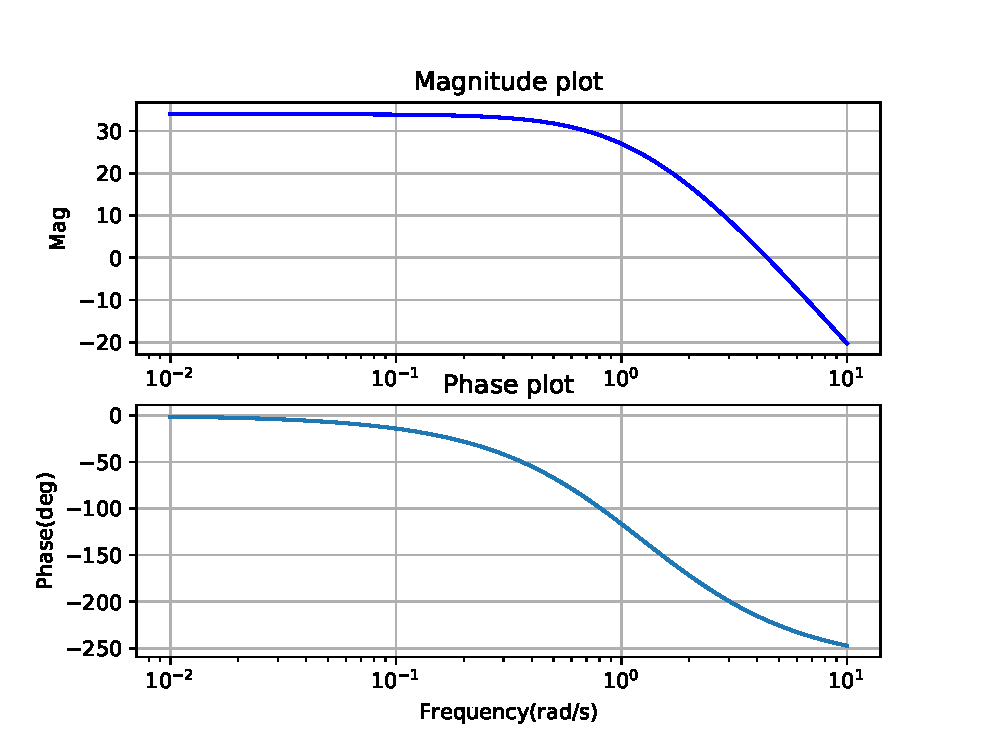
\includegraphics[width=\columnwidth]{./figures/ee18btech11017/ee18btech11017_2.eps}
%  \caption{}
%  \label{fig:ee18btech11017_2}
%\end{figure}
%
\item Since the PM in \eqref{eq:ee18btech11017_gh_pm} is negative, the closed loop system is unstable .
Verify this using the Routh-Hurwitz criterion.
%
\\
\solution 
The characteristic equation is 
\begin{align}
1+G(s)H(s)&=0 
\\
\implies s^{3}+4s^{2}+5s+102=0   
\label{eq:ee18btech11017_gh_char}
\end{align}
Constructing the routh array for \eqref{eq:ee18btech11017_gh_char},

\begin{align}
\mydet{s^3\\s^2\\s}
\mydet{1 & 5 & 0 \\ 4 & 102 & 0 \\ -20.5 & 0 & 0}
\\
\mydet{s^3\\s^2\\s\\s^0}
\mydet{1 & 5 & 0 \\ 4 & 102 & 0 \\ -20.5 & 0 & 0 \\ 102 & 0 & 0}
\end{align}

$\because $ there are two sign changes in the first column of the routh array,  two  poles lie on right half of s-plane.  Therefore,the system is unstable.


\end{enumerate}




\end{document}


